\documentclass[aspectratio=169]{beamer}

\usetheme{Madrid}
\usecolortheme{whale}

\usepackage[utf8]{inputenc}
\usepackage[greek,english]{babel}
\usepackage[LGR,T1]{fontenc}
\usepackage{lmodern}
\usepackage{substitutefont}
\substitutefont{LGR}{\rmdefault}{neohellenic}
\usepackage{graphicx}
\usepackage{amsmath}
\usepackage{amssymb}
\usepackage{booktabs}
\usepackage{multicol}
\usepackage{multirow}
\usepackage{array}
\usepackage{hyperref}
\hypersetup{hidelinks}
\usepackage{tikz}
\usetikzlibrary{arrows.meta, positioning}

% Custom Colors & Styles
\definecolor{tucblue}{RGB}{0, 51, 102}
\definecolor{tucred}{RGB}{153, 0, 0}
\definecolor{darkgreen}{RGB}{0, 128, 0}
\definecolor{tucgray}{RGB}{100, 110, 120}
\definecolor{tucdark}{RGB}{20, 30, 45}
\setbeamercolor{structure}{fg=tucblue}
\setbeamercolor{block title}{bg=tucblue,fg=white}
\setbeamercolor{block body}{bg=tucblue!5,fg=black}
\setbeamercolor{block title alerted}{bg=tucred,fg=white}
\setbeamercolor{block body alerted}{bg=tucred!5,fg=black}
\setbeamercolor{block title example}{bg=darkgreen!80!black,fg=white}
\setbeamercolor{block body example}{bg=darkgreen!5,fg=black}

% Metadata
\title[Investigating FDA in Federated LoRA Architectures]{Investigating the applicability of Federated Dynamic Averaging in Federated Low-Rank Adaptation Architectures}
\subtitle{Diploma Thesis Presentation}
\author[Asterinos Karalis]{
    \textbf{Asterinos Karalis}\\[0.3em]
    \footnotesize
    \textbf{Supervisor:} Assoc.~Prof.~Vasilis Samoladas\\[0.1em]
    \textbf{Committee:} Prof.~Antonios Deligiannakis, Prof.~Minos Garofalakis
}
\institute[]{
    \href{https://www.ece.tuc.gr/}{School of Electrical \& Computer Engineering}\\
    \href{https://www.tuc.gr/}{Technical University of Crete}
}
\date[November 2026]{November 2026}
\titlegraphic{}

\AtBeginSection[]
{
    \begin{frame}{Table of Contents}
        \tableofcontents[currentsection]
    \end{frame}
}

\begin{document}

% ==============================================================================
% Title
% ==============================================================================
\begin{frame}[plain]
    \vspace{-0.2em}
    %% Institutional Masthead: TUC Logo + University & School
    \begin{columns}[c]
        \begin{column}{0.10\textwidth}
            \href{https://www.tuc.gr/}{
\includegraphics[height=1.35cm,keepaspectratio]{tuc_logo.png}}
        \end{column}
        \begin{column}{0.88\textwidth}
            {\large \href{https://www.tuc.gr/}{\textbf{\color{tucblue}TECHNICAL UNIVERSITY OF CRETE}}}\\[0.18em]
            {\small \href{https://www.ece.tuc.gr/}{\color{tucgray}School of Electrical \& Computer Engineering}}
        \end{column}
    \end{columns}
    
    \vspace{0.4em}
    {\color{tucblue!30}\hrule height 0.8pt}
    \vspace{1.1em}
    
    %% Title Block: Clean, unboxed, balanced typography
    \centering
    {\Large \textbf{\color{tucblue} Investigating the Applicability of Federated Dynamic Averaging\\[0.3em] in Federated Low-Rank Adaptation Architectures}}\\[0.7em]
    {\small \textbf{\color{tucred} Diploma Thesis Presentation}}\\[0.8em]
    
    {\color{tucblue!20}\rule{0.6\textwidth}{0.6pt}}
    \vspace{1.0em}
    
    %% Personnel: Two balanced academic columns
    \begin{columns}[t]
        \begin{column}{0.44\textwidth}
            {\small \textbf{\color{tucblue} Author}}\\[0.4em]
            {\normalsize \textbf{\color{tucdark} Asterinos Karalis}}
        \end{column}
        
        \begin{column}{0.52\textwidth}
            {\small \textbf{\color{tucblue} Examination Committee}}\\[0.4em]
            \small
            \begin{tabular}{@{}ll@{}}
                \textbf{\color{tucdark}Supervisor:} & Assoc.~Prof.~Vasilis Samoladas \\[0.3em]
                \textbf{\color{tucdark}Members:}    & Prof.~Antonios Deligiannakis \\[0.2em]
                                                    & Prof.~Minos Garofalakis
            \end{tabular}
        \end{column}
    \end{columns}
    
    \vfill
    {\scriptsize \color{tucgray} Chania, Greece \quad$\cdot$\quad November 2026}
    \vspace{0.3em}
\end{frame}

\begin{frame}{Table of Contents}
    \tableofcontents
\end{frame}


% ==============================================================================
% SECTION 1: Background Knowledge & Problem Statement
% ==============================================================================
\section{Background Knowledge \& Problem Statement}

\begin{frame}{Background Knowledge : Distributed Learning, FedAvg \& Client Drift}
    \vspace{-0.3em}
    \begin{columns}
        \begin{column}{0.55\textwidth}
            \begin{itemize}
                \footnotesize
                \item \textbf{Federated Learning (FL)}: Privacy-preserving collaborative optimization of foundation models without centralizing client data.
                \item \textbf{Federated Averaging (FedAvg)}:
                {\small $$w_{t+1} = w_t + \frac{1}{|S_t|} \sum_{k \in S_t} \Delta_t^{(k)}$$}
                Clients execute $\tau$ local SGD steps on private data $\mathcal{D}_k$.
                \item \textbf{Statistical Heterogeneity (Non-IID)}:
                Client distributions differ in label, quantity, or features. Modeled via \textbf{Dirichlet distribution} $p_k \sim \text{Dir}(\alpha)$.
                \item \textbf{Client Drift}: Divergent local minima pull updates away from the true global optimum.
            \end{itemize}
        \end{column}
        \begin{column}{0.42\textwidth}
            \begin{block}{Dirichlet Heterogeneity ($\alpha$)}
                \footnotesize
                \begin{itemize}
                    \item $\alpha \to 0$: Extreme label skew (clients hold single-class data).
                    \item $\alpha \to \infty$: Uniform IID distribution.
                    \item Key benchmark lever for evaluating drift robustness.
                \end{itemize}
            \end{block}
            \vspace{0.2em}
            \begin{block}{The Dual Communication Bottleneck}
                \footnotesize
                \begin{itemize}
                    \item \textbf{Spatial}: Model parameter volume (billions of weights).
                    \item \textbf{Temporal}: Rigid synchronization cadence ($\tau = E$).
                \end{itemize}
            \end{block}
        \end{column}
    \end{columns}
\end{frame}

\begin{frame}{Background Knowledge : Low-Rank Adaptation (LoRA)}
    \vspace{-0.3em}
    \begin{columns}
        \begin{column}{0.55\textwidth}
            \begin{itemize}
                \footnotesize
                \item Pre-trained weights $W_0 \in \mathbb{R}^{d_{\text{out}} \times d_{\text{in}}}$ are kept \textbf{frozen}.
                \item Updates factorized into low-rank matrices:
                $$\Delta W = \frac{\alpha_{\text{lora}}}{r} B A, \quad A \in \mathbb{R}^{r \times d_{\text{in}}}, \, B \in \mathbb{R}^{d_{\text{out}} \times r}$$
                where rank $r \ll \min(d_{\text{in}}, d_{\text{out}})$.
                \item Forward pass: $h = W_0 x + \frac{\alpha_{\text{lora}}}{r} B A x$.
                \item Trainable parameters reduced by $>99\%$ with zero inference latency overhead.
                \item \textbf{Structural \& Initialization Asymmetry}:
                \begin{itemize}
                    \item \textbf{Down-Projection} $A \sim \mathcal{N}(0, \sigma^2)$: Compresses inputs to rank $r$.
                    \item \textbf{Up-Projection} $B = 0$: Expands to $d_{\text{out}}$ (ensures $\Delta W = 0$ at $t=0$).
                    \item \textbf{Asymmetric Gradients}: At onset, $\nabla_A \mathcal{L} \propto B^\top \nabla_h \mathcal{L} = 0$ while $\nabla_B \mathcal{L} \neq 0$, inducing divergent drift scales across $A$ and $B$.
                \end{itemize}
            \end{itemize}
        \end{column}
        \begin{column}{0.42\textwidth}
            \centering
            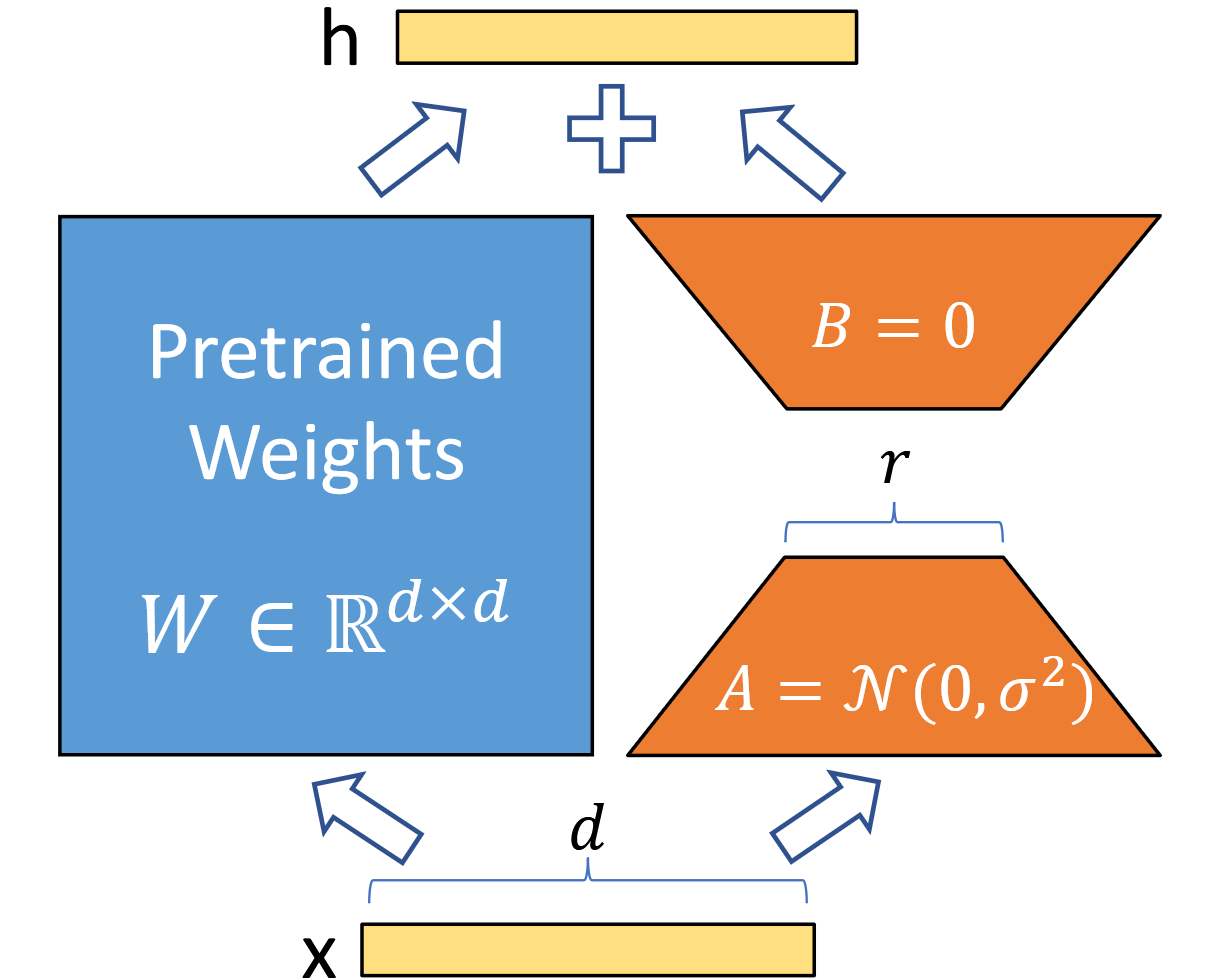
\includegraphics[width=0.88\textwidth,height=4.6cm,keepaspectratio]{figures/lora_figure.png}\\[0.2em]
            {\footnotesize \textbf{Figure}: LoRA decomposition with frozen weights $W_0$ (Hu et al., 2022).}
        \end{column}
    \end{columns}
\end{frame}

\begin{frame}{Background Knowledge : The LoRA Aggregation Inconsistency Problem}
    \begin{alertblock}{Mathematical Non-Commutativity (Bilinear Distortion)}
        Independent server-side averaging of client low-rank factors fails to reconstruct the composite weight update:
        $$\frac{1}{N}\sum_{i=1}^{N} (B_i A_i) \neq \left(\frac{1}{N}\sum_{i=1}^{N} B_i\right) \left(\frac{1}{N}\sum_{i=1}^{N} A_i\right)$$
    \end{alertblock}
    
    \begin{itemize}
        \item Direct FedAvg on $(B_i, A_i)$ induces cross-client geometric interference.
        \item Destabilizes convergence under non-IID data distributions (Yang et al., IJCAI 2025).
        \item \textbf{Prior Work Limitations}:
        \begin{itemize}
            \item \emph{Full-matrix expansion} ($\Delta W = BA$): Transmits full parameter matrices $\to$ destroys spatial savings.
            \item \emph{FFA-LoRA}: Permanently freezes down-projection $A$ $\to$ sacrifices adapter expressivity.
            \item \emph{FLoRA}: Server-side SVD recalculation $\to$ high server compute overhead.
        \end{itemize}
    \end{itemize}
\end{frame}
\begin{frame}{Background Knowledge : Robust Low-Rank Adaptation (RoLoRA)}
    \framesubtitle{Chen et al., NeurIPS 2025 -- Alternating Coordinate Optimization}
    \vspace{-0.3em}
    \begin{block}{Alternating Coordinate Optimization Restores Aggregation Linearity}
        \footnotesize
        \textbf{RoLoRA} resolves the bilinear inconsistency by alternating the active trainable matrix while freezing the other globally across all clients:
        \begin{itemize}
            \item \textbf{Even Rounds (Train $B$, Freeze $A$)}:
            $\frac{1}{N}\sum_{i=1}^N (B_i A) = \left(\frac{1}{N}\sum_{i=1}^N B_i\right) A = \bar{B} A$
            \item \textbf{Odd Rounds (Train $A$, Freeze $B$)}:
            $\frac{1}{N}\sum_{i=1}^N (B A_i) = B \left(\frac{1}{N}\sum_{i=1}^N A_i\right) = B \bar{A}$
            \item \textbf{Core Limitation}: Enforces a rigid, static local epoch schedule ($E$), leaving temporal synchronization completely unoptimized.
        \end{itemize}
    \end{block}
    \vspace{0.1em}
    
    \centering
    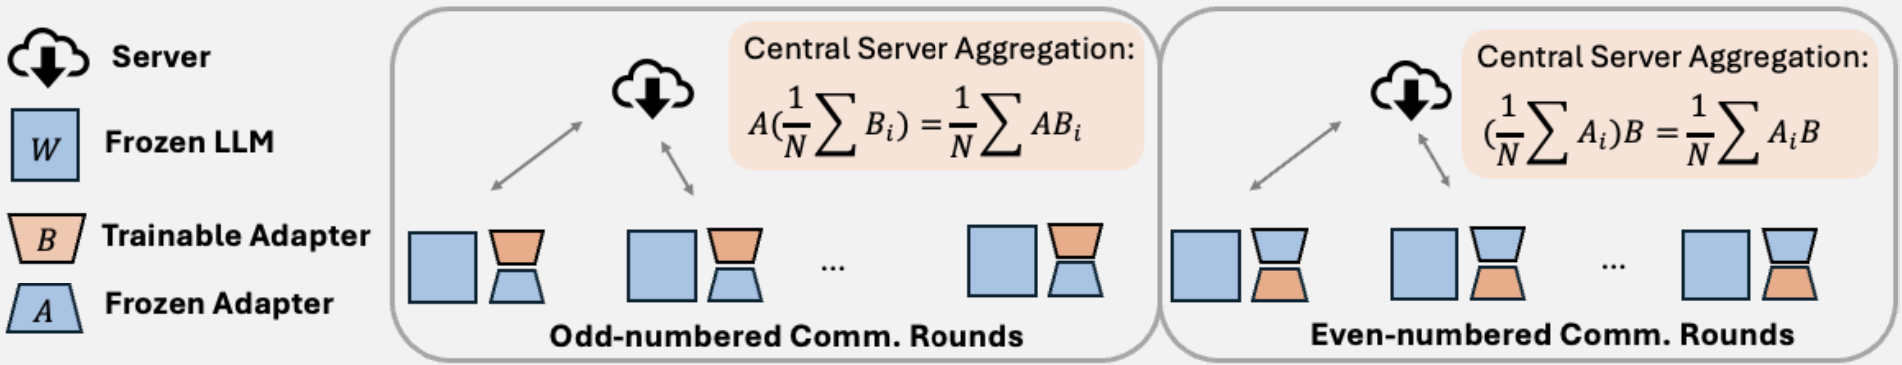
\includegraphics[width=0.90\textwidth,height=1.75cm,keepaspectratio]{figures/rolora_framework.png}\\[0.1em]
    {\scriptsize \textbf{Figure}: RoLoRA alternating framework across communication rounds (Chen et al. schematic uses row-vector $AB$ notation; thesis follows standard column-vector $BA$ convention).}
\end{frame}
\begin{frame}{Background Knowledge : FDA-Opt \& Geometric Monitoring}
    \framesubtitle{Theologitis, Samoladas \& Deligiannakis, 2025 -- Dynamic Variance Halting}
    \begin{columns}
        \begin{column}{0.55\textwidth}
            \begin{itemize}
                \footnotesize
                \item \textbf{Geometric Monitoring Root}: Decomposes global threshold functions over distributed streams into local \textbf{safe zones} (Sharfman et al., 2006).
                \item \textbf{FDA-Opt Formulation} (Theologitis et al., 2025): Tracks client update dispersion via parameter variance:
                {\small $$\text{Var}(W_{t,i}) = \frac{1}{|S_t|}\sum_{k \in S_t} \|\Delta_{t,i}^{(k)}\|_2^2 - \|g_{t,i}\|_2^2$$}
                Low variance $=$ aligned progress; high variance $=$ client drift.
                \item \textbf{Event-Driven Halting}: Synchronize when $\text{Var}(W) > \theta_t$.
                \item \textbf{Midpoint Threshold Scaling}: $\theta_{t+1} = \text{var}_t \cdot \frac{\tau}{2 s_t}$.
            \end{itemize}
        \end{column}
        \begin{column}{0.43\textwidth}
            \begin{block}{Research Gap in FDA-Opt}
                \footnotesize
                \begin{itemize}
                    \item FDA-Opt operated strictly on \textbf{full model parameters} (approximated via AMS sketches).
                    \item Spatial compression (LoRA) and temporal adaptivity (FDA) had never been synthesized.
                    \item Low-rank adapters exhibit high variance volatility requiring decoupled mechanics.
                \end{itemize}
            \end{block}
        \end{column}
    \end{columns}
\end{frame}

\begin{frame}{Background Knowledge : Synthesis of Foundational Precursors}
    \framesubtitle{Synthesizing RoLoRA (Spatial) and FDA-Opt (Temporal)}
    \centering
    \scriptsize
    \renewcommand{\arraystretch}{1.15}
    \resizebox{\textwidth}{!}{%
\begin{tabular}{l l l l}
        \toprule
        \textbf{Dimension} & \textbf{RoLoRA} (NeurIPS '25) & \textbf{FDA-Opt} (2025) & \textbf{FDA-RoLoRA} (\textbf{This Thesis}) \\
        \midrule
        \textbf{Optimization Focus} & Spatial parameter volume & Temporal synchronization & \textbf{Joint Spatial + Temporal} \\
        \textbf{Parameter Scope} & Low-rank adapters ($A, B$) & Full model weights & \textbf{Low-rank adapters ($A, B$)} \\
        \textbf{Aggregation} & Alternating coordinates & Standard FedAvg / FedOpt & \textbf{Alternating coordinates} \\
        \textbf{Local Scheduling} & Static fixed ($E$ epochs) & Dynamic (Model variance) & \textbf{Dynamic (Subspace variance)} \\
        \textbf{Variance Tracking} & None & Full-weight (AMS sketch) & Exact in simulation (monitoring cost not evaluated) \\
        \textbf{Threshold Logic} & None & Single scalar threshold & \textbf{Decoupled Dual-Track} $(\theta_A, \theta_B)$ \\
        \bottomrule
    \end{tabular}}
    
    \vspace{0.7em}
    \begin{alertblock}{Complementary Synergy}
        \scriptsize
        \textbf{FDA-RoLoRA} solves the core limitations of both parent papers: RoLoRA provides the strict aggregation linearity needed for stable variance tracking, while FDA-Opt provides the event-driven cadence needed to eliminate static schedule waste.
    \end{alertblock}
\end{frame}


% ==============================================================================
% SECTION 2: Proposed Methodology: FDA-RoLoRA
% ==============================================================================
\section{Proposed Methodology: FDA-RoLoRA}

\begin{frame}{Methodology : Dynamic Averaging in Federated LoRA}
    \begin{block}{Taxonomy of Integration Avenues}
        Different PEFT architectures have distinct mathematical structures and optimization geometries; dynamic averaging cannot use a single one-size-fits-all rule.
    \end{block}
    
    \begin{itemize}
        \item \textbf{FDA + FedAvg-LoRA}: Dynamic averaging with simultaneous $(A, B)$ training.
        \begin{itemize}
            \item \emph{Drawback}: Inherits bilinear aggregation error; non-linear distortion destabilizes variance monitoring.
        \end{itemize}
        \item \textbf{FDA + FFA-LoRA}: Dynamic averaging with permanently frozen $A$ \emph{[Future Work]}.
        \item \textbf{FDA + SLoRA}: Dynamic thresholding over sparse adapter coordinates \emph{[Future Work]}.
        \item \textbf{FDA-RoLoRA}: \textbf{This Thesis}
        \begin{itemize}
            \item Synthesizes \textbf{RoLoRA} (Chen et al., 2025) and \textbf{FDA-Opt} (Theologitis et al., 2025).
            \item Alternating coordinates provide strict linearity $\to$ perfect substrate for variance tracking.
            \item Maintains independent persistent variance thresholds $(\theta_A, \theta_B)$ for each subspace.
        \end{itemize}
    \end{itemize}
\end{frame}

\begin{frame}{Methodology : FDA-RoLoRA Architecture}
    \vspace{-0.3em}
    \begin{block}{Decoupled Dual-Track Subspace Variance Mechanics}
        \footnotesize
        RoLoRA isolates the optimization trajectories of down-projection ($A$) and up-projection ($B$). Because $A$ and $B$ exhibit severe gradient scale disparity ($\theta_B \gg \theta_A$), FDA-RoLoRA maintains two persistent, decoupled threshold tracks $(\theta_A, \theta_B)$.
    \end{block}
    
    \footnotesize
    \begin{itemize}
        \item \textbf{Active Subspace Mapping}: Server maps active threshold based on designated matrix $\mathcal{M}^{(r)} \in \{B, A\}$ ($B$-first schedule):
        $$\theta_{\text{current}}^{(r)} = \begin{cases} \theta_A & \text{if } \mathcal{M}^{(r)} = A \\ \theta_B & \text{if } \mathcal{M}^{(r)} = B \end{cases}$$
        \item \textbf{Direct Subspace Variance}: Evaluated exclusively on low-rank coordinate tensors:
        $$\text{Var}_{\text{subspace}}(\Delta^{(e)}) = \frac{1}{|S_r|} \sum_{i \in S_r} \|\Delta_i^{(e)}\|_2^2 - \left\| \frac{1}{|S_r|} \sum_{i \in S_r} \Delta_i^{(e)} \right\|_2^2$$
        \item Eliminates memory and compute overhead of projecting drifts back to full weight space $\Delta W = \frac{\alpha}{r}BA$.
    \end{itemize}
\end{frame}

\begin{frame}{Methodology : Independent Halting \& Local Training Bounds}
    \vspace{-0.35em}
    \begin{columns}
        \begin{column}{0.50\textwidth}
            \begin{block}{Local Epoch Bounds ($[e_{\min}, e_{\max}]$)}
                \scriptsize
                Client training bounded in $[e_{\min}, e_{\max}]$ with operational floor $e_{\min}$ to guarantee baseline progress:
                $$\text{Halt if } \text{Var}_{\text{subspace}}(\Delta^{(e)}) > \theta_{\text{current}}^{(r)} \;\lor\; e \ge e_{\max}$$
                Evaluated at epoch boundaries $e \ge e_{\min}$.
            \end{block}
            \vspace{-0.3em}
            \begin{block}{Operational Progress Floor ($e_{\min} = 1$)}
                \scriptsize
                \begin{itemize}
                    \item Ensures clients execute at least one local epoch before variance checks begin.
                    \item Both tracks initialize $\theta_A = \theta_B = 0$, calibrating baseline variance at $e^* = 1$ in rounds $0$ and $1$.
                \end{itemize}
            \end{block}
        \end{column}
        \begin{column}{0.48\textwidth}
            \begin{block}{Subspace Monitoring}
                \scriptsize
                Calculated exclusively on the active low-rank coordinate matrix ($A$ or $B$):
                $$\text{Var}_{\text{subspace}}(\Delta^{(e)}) = \frac{1}{|S_r|} \sum_{i \in S_r} \|\Delta_i^{(e)} - \bar{\Delta}^{(e)}\|_2^2$$
                \begin{itemize}
                    \item Evaluated over $<0.5\%$ of backbone parameters ($120\,\text{KB}$ per active track vs.\ $500\,\text{MB}$ full model).
                    \item With sketches in a deployment, the full adapter uplink (120 KB) would be sent once per round at $e^*$. Sketches were not run in these experiments.
                \end{itemize}
            \end{block}
        \end{column}
    \end{columns}
    \vspace{0.1em}
    \begin{alertblock}{Simulation vs. Deployment}
        \scriptsize
        In simulation, exact low-rank variance is computed directly in memory. A real deployment must send monitoring data at every epoch check. This cost is not included in the reported MB.
    \end{alertblock}
\end{frame}

\begin{frame}{Methodology : Coordinate-Wise FedAvg \& Protocol Flow}
    \vspace{-0.4em}
    \begin{columns}
        \begin{column}{0.48\textwidth}
            \begin{block}{Coordinate-Wise FedAvg Aggregation}
                \begin{itemize}
                    \footnotesize
                    \item Client drift: $\Delta_i^{(e^*)} = W_{i, e^*}^{(r)} - W_{\text{act}}^{(r)}$
                    \item Cohort average: $\bar{\Delta}^{(r)} = \frac{1}{|S_r|}\sum_{i \in S_r} \Delta_i^{(e^*)}$
                    \item Linear FedAvg update ($\eta_s = 1.0$):
                    $$W_{\text{act}}^{(r+1)} = W_{\text{act}}^{(r)} + \bar{\Delta}^{(r)}$$
                    \item \textbf{Linear Aggregation}: Standard FedAvg avoids momentum artifacts, isolating gains strictly to dynamic variance tracking.
                \end{itemize}
            \end{block}
        \end{column}
        \begin{column}{0.48\textwidth}
            \begin{block}{Protocol Execution Lifecycle}
                \begin{enumerate}
                    \footnotesize
                    \item \textbf{Toggle}: Server selects active track $A$ or $B$.
                    \item \textbf{Broadcast}: Sends $W_{\text{act}}^{(r)}$ and $\theta_{\text{current}}^{(r)}$ to $S_r$.
                    \item \textbf{Train}: Clients run local SGD steps ($\eta_c = 0.1$).
                    \item \textbf{Check}: Evaluate subspace variance at $e \ge e_{\min}$ (exact and in memory in simulation; a deployment must send monitoring data at each check).
                    \item \textbf{Halt}: Return $\Delta_i^{(e^*)}$ when $\text{Var} > \theta$ or $e = e_{\max}$.
                    \item \textbf{Aggregate}: Server averages client drifts ($\bar{\Delta}^{(r)}$).
                    \item \textbf{Evolve}: Update active threshold $\theta_{\mathcal{M}^{(r)}}^{(\text{next})}$.
                    \item \textbf{Step}: Server applies FedAvg to active coordinate.
                \end{enumerate}
            \end{block}
        \end{column}
    \end{columns}
\end{frame}


% ==============================================================================
% SECTION 3: System Implementation
% ==============================================================================
\section{System Implementation}

\begin{frame}{Implementation : Modular 3-Tier Software Architecture}
    \begin{columns}[t]
        \begin{column}{0.32\textwidth}
            \begin{block}{1. Server Orchestrator}
                \footnotesize
                \begin{itemize}
                    \item Global $A, B$ matrices.
                    \item Tracks $(\theta_A, \theta_B)$ state.
                    \item Coordinates RoLoRA toggle.
                    \item Coordinate-wise FedAvg.
                \end{itemize}
            \end{block}
        \end{column}
        \begin{column}{0.32\textwidth}
            \begin{block}{2. Client Nodes}
                \footnotesize
                \begin{itemize}
                    \item Private data partitions.
                    \item Local SGD training loops.
                    \item Subspace drift computation.
                    \item Variance checks at $e \ge e_{\min}$.
                \end{itemize}
            \end{block}
        \end{column}
        \begin{column}{0.32\textwidth}
            \begin{block}{3. Comm. Interface}
                \footnotesize
                \begin{itemize}
                    \item Low-rank serialization.
                    \item PyTorch, HF \& PEFT.
                    \item Lightweight FDA-Opt core.
                \end{itemize}
            \end{block}
        \end{column}
    \end{columns}
    
    \vspace{0.3em}
    \begin{block}{Key Engineering Decisions}
        \footnotesize
        \begin{itemize}
            \item \textbf{FDA-Opt Base vs. FederatedScope-LLM}: The RoLoRA paper (Chen et al., NeurIPS 2025) used FederatedScope-LLM without a public release. We adopted and extended the open-source \textbf{FDA-Opt} repository (Theologitis et al., 2025), integrating HuggingFace PEFT and RoLoRA coordinate alternation into its modular PyTorch core.
            \item \textbf{Exact Variance in Simulation}: Variance is computed exactly in memory to evaluate the synchronization rule under ideal measurement. This does not remove the need for monitoring communication in a real deployment.
        \end{itemize}
    \end{block}
\end{frame}





\section{Evaluations \& Results}

\begin{frame}[label=main_impl]{Evaluation : Experimental Setup \& Benchmark Protocol}
    \framesubtitle{Foundation Model Configuration, Low-Rank Parameterization \& Benchmark Protocol \hfill \hyperlink{backup_algo}{\beamerbutton{Algorithm}} \; \hyperlink{backup_testbed}{\beamerbutton{Hardware Details}}}
    \scriptsize
    \begin{columns}[t]
        \begin{column}{0.48\textwidth}
            \begin{block}{Model \& Low-Rank Parameterization}
                \begin{itemize}
                    \item \textbf{Model Backbone}: \texttt{roberta-base} ($125\text{M}$ params, 12 layers, 768 hidden; selected for multi-seed sweeps under hardware budget).
                    \item \textbf{Adapter Configuration}: Rank $r=4$, scaling factor $\alpha_{\text{lora}}=8$ on Query ($W_q$) and Value ($W_v$) projections across top blocks $\{7\dots 11\}$ (MNLI, QNLI, QQP) and top 3 blocks $\{9\dots 11\}$ (SST-2); \textbf{about 0.05\% trainable parameter share}.
                    \item \textbf{Bi-Directional Adapter Payload}: $240\,\text{KB}$/client/round ($4.69\,\text{MB}$ at $C=20$, $11.72\,\text{MB}$ at $C=50$); $144\,\text{KB}$ for SST-2. \textbf{Monitoring data is excluded}.
                    \item \textbf{Optimization}: Client SGD ($\eta_c = 0.1$, batch $B \in \{32, 64\}$); Server FedAvg ($\eta_s = 1.0$).
                \end{itemize}
            \end{block}
        \end{column}
        \begin{column}{0.50\textwidth}
            \begin{block}{Benchmark Regimes \& Baselines}
                \begin{itemize}
                    \item \textbf{Tasks \& Datasets}: GLUE benchmark suite (MNLI, QNLI, QQP, SST-2) capped at $\le 25{,}000$ training samples; full validation sets.
                    \item \textbf{Cohorts \& Regimes}: $C \in \{20, 50\}$ clients (full participation); Homogeneous ($\alpha=1000.0$) vs.\ Dirichlet Label Skew ($\alpha=0.5$).
                    \item \textbf{Baselines}: Fixed RoLoRA $E \in \{5, 10, 15, 20\}$ where run. Non-IID uses $E = 10$ in every configuration, plus $E = 20$ on MNLI and QNLI ($C = 20$).
                    \item \textbf{FDA-RoLoRA Settings}: $e_{\min}=1$, $e_{\max} \in \{20, 40\}$, $k \in \{0.5, 1.0\}$.
                    \item \textbf{Execution Budget}: \textbf{173 completed runs} evaluated under uniform platform (\textbf{2 seeds per configuration}).
                \end{itemize}
            \end{block}
        \end{column}
    \end{columns}
\end{frame}
\begin{frame}[label=main_scorecard]{Evaluation : Results Summary}
    \framesubtitle{All GLUE Benchmarks on \texttt{roberta-base} \hfill \hyperlink{backup_iid_table}{\beamerbutton{Full IID Table}} \; \hyperlink{backup_noniid_table}{\beamerbutton{Full Non-IID Table}}}
    \vspace{-0.55em}
    \centering
    \resizebox{0.96\textwidth}{!}{%
    \renewcommand{\arraystretch}{0.76}
    \begin{tabular}{lllccccc}
        \toprule
        \textbf{Task \& Cohort} & \textbf{Regime} & \textbf{Top FDA-RoLoRA ($e_{\min}=1$)} & \textbf{FDA Peak (\%)} & \textbf{FDA Final (\%)} & \textbf{Top RoLoRA Baseline} & \textbf{RoLoRA Peak (\%)} & \textbf{RoLoRA Final (\%)} \\
        \midrule
        \multirow{2}{*}{\textbf{MNLI} ($C=20$)} 
        & IID ($\alpha=1000$)      & FDA ($e_{\max}=20, k=1.0$) & $\mathbf{76.86 \pm 0.10}$ & $\mathbf{76.86 \pm 0.10}$ & RoLoRA ($E=10$) & $76.60 \pm 0.85$ & $76.60 \pm 0.85$ \\
        & Non-IID ($\alpha=0.5$)   & FDA ($e_{\max}=20, k=1.0$) & $\mathbf{74.47 \pm 0.11}$ & $73.71 \pm 0.77$          & RoLoRA ($E=10$) & $74.24 \pm 0.12$ & $\mathbf{74.11 \pm 0.31}$ \\
        \cmidrule{1-8}
        \multirow{2}{*}{\textbf{MNLI} ($C=50$)} 
        & IID ($\alpha=1000$)      & FDA ($e_{\max}=20, k=1.0$) & $\mathbf{69.85 \pm 3.37}$ & $\mathbf{69.85 \pm 3.37}$ & RoLoRA ($E=10$) & $65.85 \pm 2.85$ & $65.85 \pm 2.85$ \\
        & Non-IID ($\alpha=0.5$)   & FDA ($e_{\max}=20, k=0.5$) & $55.56 \pm 1.65$          & $55.23 \pm 2.11$          & RoLoRA ($E=10$) & $\mathbf{56.55 \pm 6.94}$ & $\mathbf{56.22 \pm 7.40}$ \\
        \midrule
        \multirow{2}{*}{\textbf{QNLI} ($C=20$)} 
        & IID ($\alpha=1000$)      & FDA ($e_{\max}=20, k=1.0$) & $\mathbf{83.14 \pm 0.34}$ & $67.63 \pm 22.28$         & RoLoRA ($E=10$) & $81.83 \pm 0.92$ & $\mathbf{75.03 \pm 10.54}$ \\
        & Non-IID ($\alpha=0.5$)   & FDA ($e_{\max}=20, k=1.0$) & $\mathbf{84.22 \pm 0.41}$ & $\mathbf{81.88 \pm 2.90}$ & RoLoRA ($E=10$) & $83.50 \pm 1.67$ & $81.10 \pm 4.31$ \\
        \cmidrule{1-8}
        \multirow{2}{*}{\textbf{QNLI} ($C=50$)} 
        & IID ($\alpha=1000$)      & FDA ($e_{\max}=20, k=1.0$) & $82.77 \pm 2.14$          & $82.47 \pm 1.72$          & RoLoRA ($E=20$) (1 seed) & $\mathbf{88.14 \pm 0.00}$ & $\mathbf{87.94 \pm 0.00}$ \\
        & Non-IID ($\alpha=0.5$)   & FDA ($e_{\max}=20, k=0.5$) & $\mathbf{75.69 \pm 1.66}$ & $50.13 \pm 0.94$          & RoLoRA ($E=10$) & $74.61 \pm 10.15$ & $\mathbf{58.45 \pm 12.71}$ \\
        \midrule
        \multirow{2}{*}{\textbf{QQP} ($C=20$)} 
        & IID ($\alpha=1000$)      & FDA ($e_{\max}=20, k=1.0$) & $\mathbf{78.57 \pm 4.23}$ & $\mathbf{76.34 \pm 5.33}$ & RoLoRA ($E=10$) & $75.47 \pm 1.19$ & $75.47 \pm 1.19$ \\
        & Non-IID ($\alpha=0.5$)   & FDA ($e_{\max}=20, k=1.0$) & $\mathbf{77.88 \pm 0.66}$ & $64.52 \pm 18.23$         & RoLoRA ($E=10$) & $77.69 \pm 2.18$ & $\mathbf{76.76 \pm 3.41}$ \\
        \cmidrule{1-8}
        \multirow{2}{*}{\textbf{QQP} ($C=50$)} 
        & IID ($\alpha=1000$)      & FDA ($e_{\max}=20, k=0.5$) & $73.86 \pm 0.39$          & $72.08 \pm 0.20$          & RoLoRA ($E=10$) & $\mathbf{78.79 \pm 1.38}$ & $\mathbf{75.43 \pm 1.07}$ \\
        & Non-IID ($\alpha=0.5$)   & FDA ($e_{\max}=20, k=1.0$) & $74.55 \pm 1.30$          & $57.45 \pm 11.29$         & RoLoRA ($E=10$) & $\mathbf{74.71 \pm 1.63}$ & $\mathbf{69.28 \pm 8.14}$ \\
        \midrule
        \multirow{2}{*}{\textbf{SST-2} ($C=20$)} 
        & IID ($\alpha=1000$)      & FDA ($e_{\max}=20, k=1.0$) & $92.14 \pm 0.24$          & $91.80 \pm 0.24$          & RoLoRA ($E=20$) & $\mathbf{92.55 \pm 0.30}$ & $\mathbf{92.16 \pm 0.13}$ \\
        & Non-IID ($\alpha=0.5$)   & FDA ($e_{\max}=20, k=1.0$) & $\mathbf{89.91 \pm 0.81}$ & $69.72 \pm 29.19$         & RoLoRA ($E=10$) & $89.62 \pm 1.87$ & $\mathbf{89.62 \pm 1.87}$ \\
        \cmidrule{1-8}
        \multirow{2}{*}{\textbf{SST-2} ($C=50$)} 
        & IID ($\alpha=1000$)      & FDA ($e_{\max}=20, k=1.0$) & $89.68 \pm 1.14$          & $89.68 \pm 1.14$          & RoLoRA ($E=20$) & $\mathbf{92.01 \pm 0.57}$ & $\mathbf{91.90 \pm 0.37}$ \\
        & Non-IID ($\alpha=0.5$)   & FDA ($e_{\max}=20, k=1.0$) & $\mathbf{85.95 \pm 5.60}$ & $\mathbf{81.36 \pm 9.97}$ & RoLoRA ($E=10$) & $59.00 \pm 11.11$ & $53.33 \pm 3.08$ \\
        \bottomrule
    \end{tabular}%
    }
    
    \vspace{0.15em}
    {\tiny \textit{Table Note}: QNLI $C=20$ Non-IID: RoLoRA $E=20$ final accuracy is $82.97 \pm 0.50$.}
    
    \vspace{0.2em}
    \begin{exampleblock}{Key Empirical Takeaways}
        \tiny
        \textbf{Peak vs.\ Final}: Against each configuration's best static baseline, FDA-RoLoRA wins 10 of 16 on peak accuracy but 4 of 16 on final accuracy (Non-IID: 6 of 8 vs.\ 1 of 8).\\
        \textbf{MNLI Non-IID ($C = 20$)}: Reaches RoLoRA $E = 10$ final accuracy in 13--30\% fewer rounds, while avoiding the $E = 20$ post-peak drop ($73.31\% \to 68.87\%$). A byte saving is not established once monitoring is counted.\\
        \textbf{Plateau Escape on SST-2 Non-IID ($C=50$)}: Static RoLoRA trapped near majority-class ($59.00\%$ peak, $53.33\%$ final); FDA dynamically expands compute ($\bar{e}=14.57$) to reach $\mathbf{85.95\%}$ peak ($\mathbf{+26.95\%}$ gain).
    \end{exampleblock}
\end{frame}
\begin{frame}[label=main_iid]{Evaluation : Homogeneous Consensus (IID, $\alpha=1000.0$)}
    \framesubtitle{No Consistent Advantage: The Controller Undershoots Its Target \hfill \hyperlink{backup_iid_mnli_qnli}{\beamerbutton{MNLI/QNLI Plots}} \; \hyperlink{backup_iid_qqp_sst2}{\beamerbutton{QQP/SST-2 Plots}}}
    \vspace{-0.55em}
    \begin{columns}
        \begin{column}{0.48\textwidth}
            \begin{block}{Optimization Dynamics \& Controller Behavior}
                \tiny
                \begin{itemize}
                    \item \textbf{Consensus}: Updates align along shared trajectory ($\bar{\nu} \le 1.58$).
                    \item \textbf{Super-Linear Drift Surge}: In compact low-rank subspaces, coordinate variance grows super-linearly ($\text{Var}_{\text{subspace}}(t) \propto t^p, \, p > 1$).
                    \item \textbf{Setpoint Undershoot}: Breaches linear predictor early $\to$ systematic undershoot ($\bar{e} \approx 5.8\text{--}7.8$ for $k=0.5$; $\bar{e} \approx 9.1\text{--}13.4$ for $k=1.0$).
                \end{itemize}
            \end{block}
            \vspace{-0.4em}
            \begin{exampleblock}{Observations}
                \tiny
                \begin{itemize}
                    \item \textbf{QQP ($C=50$)}: Stops early at rd 14 at a lower plateau ($72.65\%$ final, $73.63\%$ peak) vs.\ RoLoRA $E=10$ ($75.43\%$ final, $78.79\%$ peak) $\to$ earlier plateau, not bandwidth saving at parity.
                    \item \textbf{MNLI ($C=50$)}: Deeper compute ($\bar{e}=12.15$) breaks static $E=10$ plateau ($69.85\%$ vs.\ $65.85\%$).
                    \item \textbf{Takeaway}: FDA-RoLoRA shows no consistent advantage over fixed-epoch RoLoRA under IID data.
                \end{itemize}
            \end{exampleblock}
        \end{column}
        
        \begin{column}{0.50\textwidth}
            \centering
            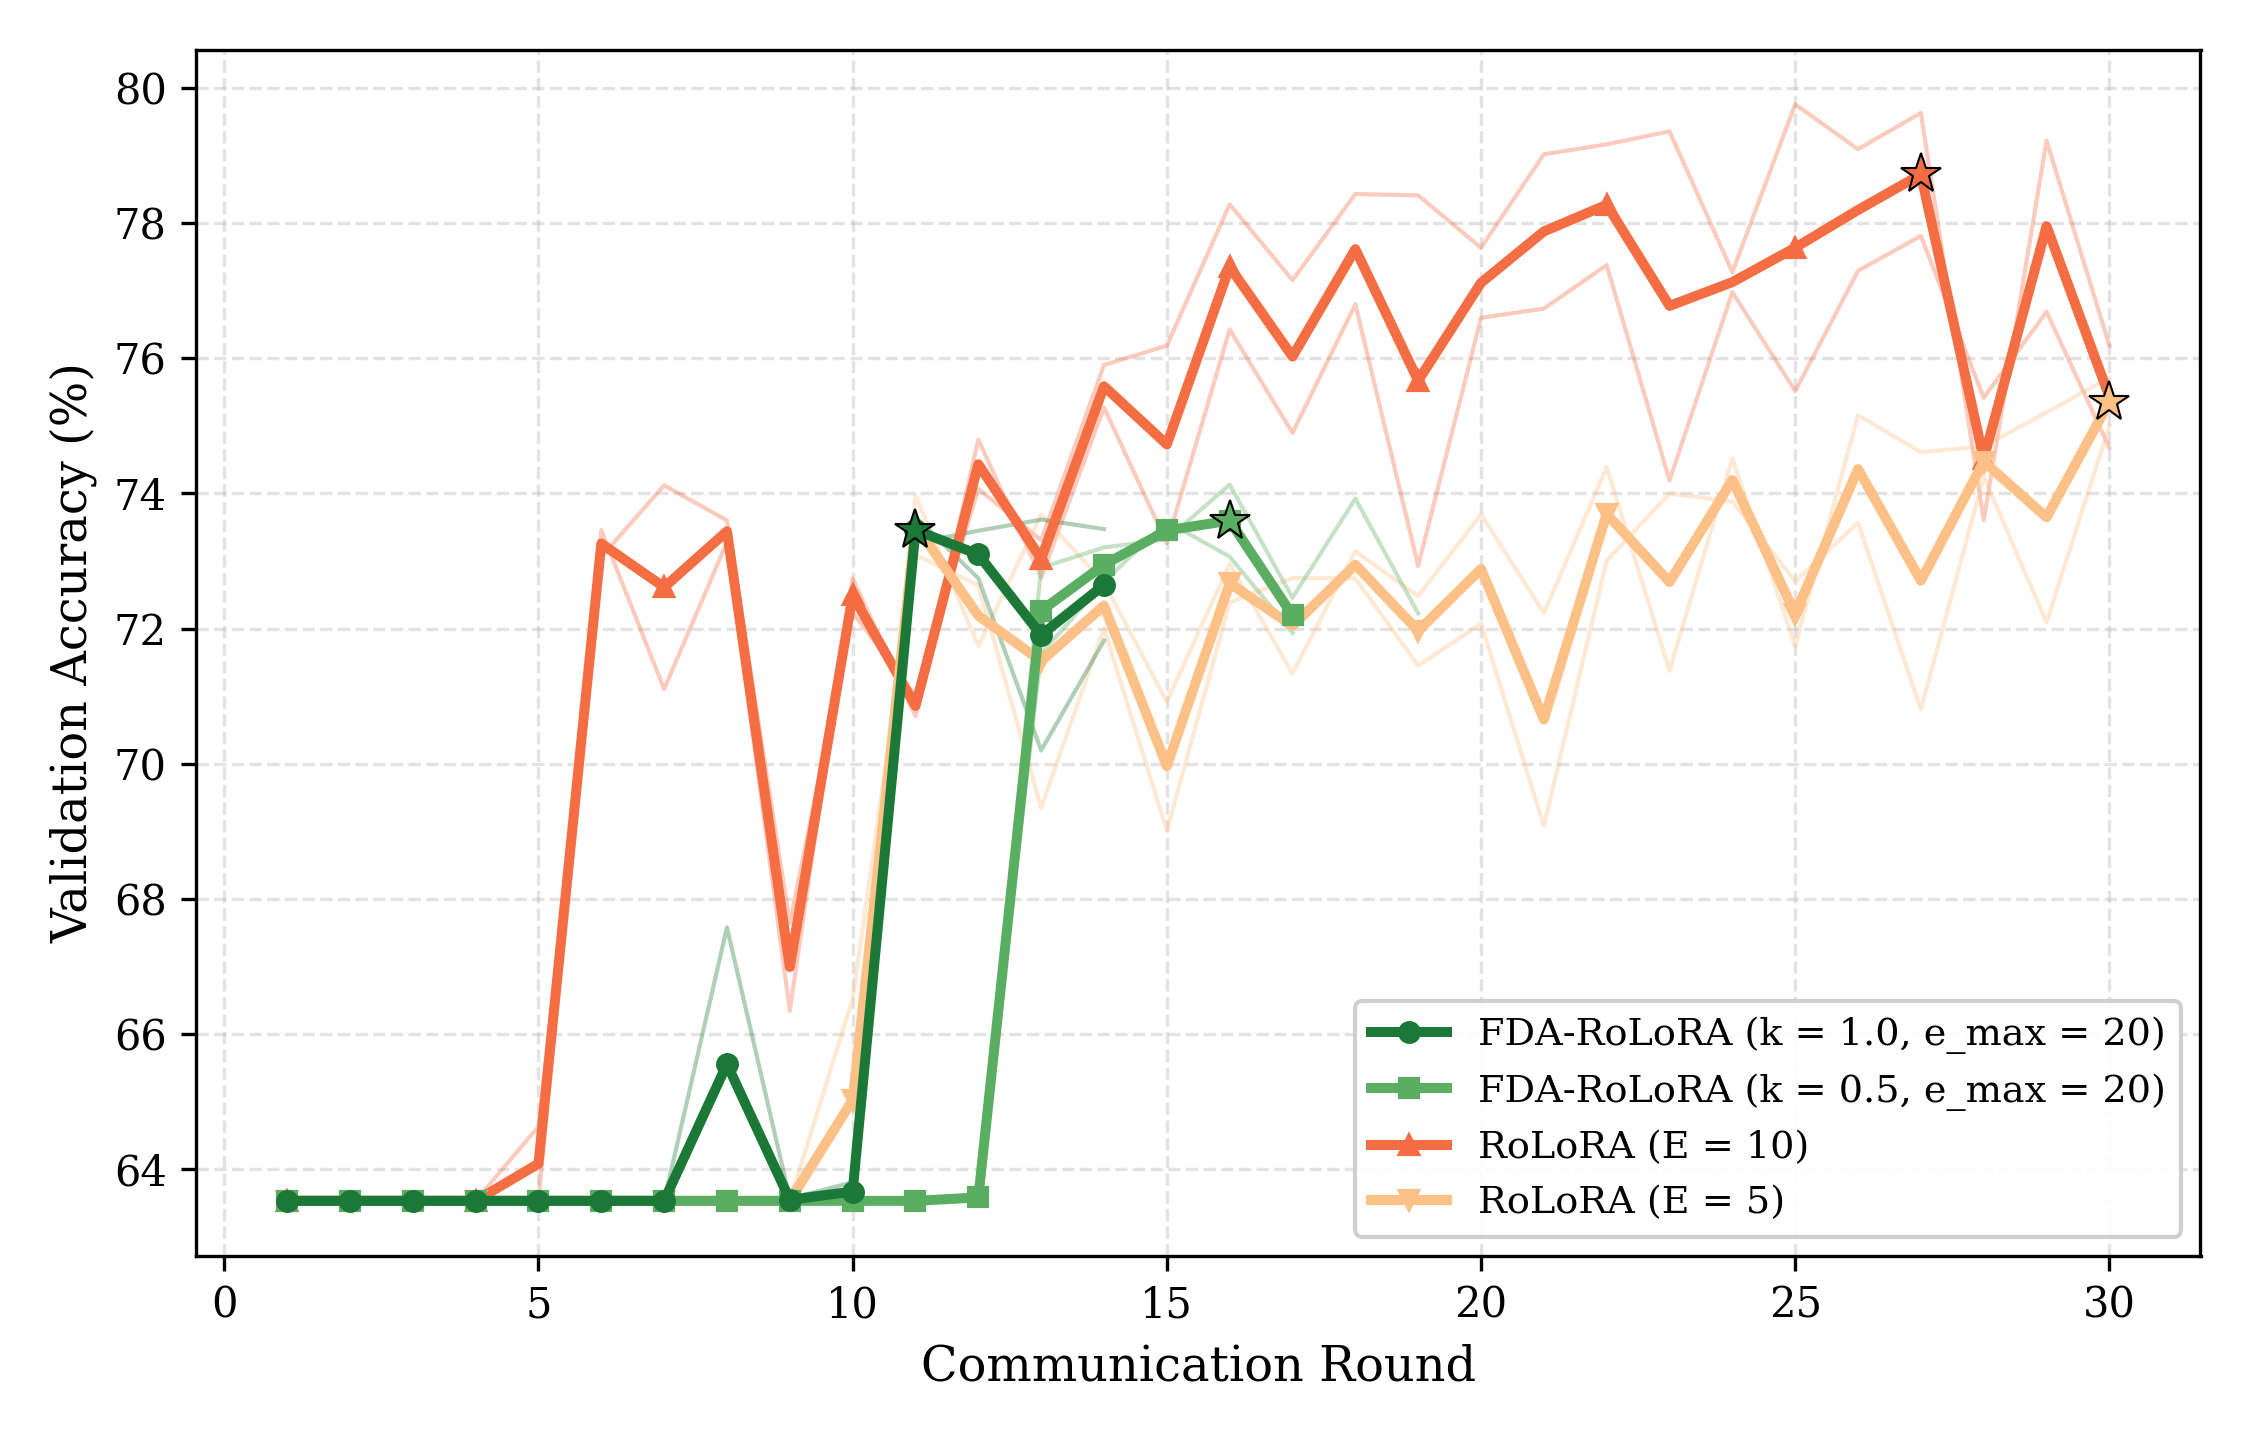
\includegraphics[width=\linewidth,height=0.62\textheight,keepaspectratio]{figures/10_QQP_C50_R30_LR0.1_1_accuracy.png}
            \vspace{-0.2em}
            \tiny \textbf{Figure}: Validation accuracy vs.\ communication rounds on QQP ($C=50$, IID).
        \end{column}
    \end{columns}
\end{frame}
\begin{frame}[label=main_noniid]{Evaluation : Statistical Heterogeneity (Non-IID, $\alpha=0.5$)}
    \framesubtitle{Where FDA-RoLoRA Helps: Plateau Escape and Fewer MNLI Rounds \hfill \hyperlink{backup_noniid_mnli}{\beamerbutton{MNLI \& Epoch Plots}}}
    \vspace{-0.55em}
    \begin{columns}
        \begin{column}{0.48\textwidth}
            \begin{alertblock}{Controller Behaviour Under Label Skew}
                \tiny
                \begin{itemize}
                    \item Gradient dispersion across skewed client classes linearizes drift accumulation across local epochs.
                    \item Controller tracks nominal setpoint closely ($\mathcal{S} \approx 0.91\text{--}1.11$, $\bar{e} \approx 8.7\text{--}10.9$ for $k=0.5$ and $\bar{e} \approx 13.0\text{--}17.5$ for $k=1.0$).
                    \item Expands local training when variance is low and synchronizes earlier when it rises. This did not prevent late accuracy drops.
                \end{itemize}
            \end{alertblock}
            \vspace{-0.4em}
            \begin{block}{Empirical Highlights}
                \tiny
                \begin{itemize}
                    \item \textbf{SST-2 ($C=50$)}: RoLoRA ($E=10$) trapped near majority class ($59.00\%$ peak, $53.33\%$ final); FDA expands compute ($\bar{e}=14.57$) to reach $\mathbf{85.95\%}$ peak ($\mathbf{+26.95\%}$ gain!).
                    \item \textbf{MNLI ($C = 20$)}: Reaches RoLoRA $E = 10$ final accuracy in 13--30\% fewer rounds and avoids the $E = 20$ post-peak drop.
                    \item \textbf{QNLI}: Reaches $84.22\%$ peak at $C = 20$. At $C = 50$, it reaches $75.69\%$ peak with $k = 0.5$ (RoLoRA: $74.61\%$), but both FDA-RoLoRA variants end near chance ($49.51\%$ and $50.13\%$).
                \end{itemize}
            \end{block}
        \end{column}
        
        \begin{column}{0.50\textwidth}
            \centering
            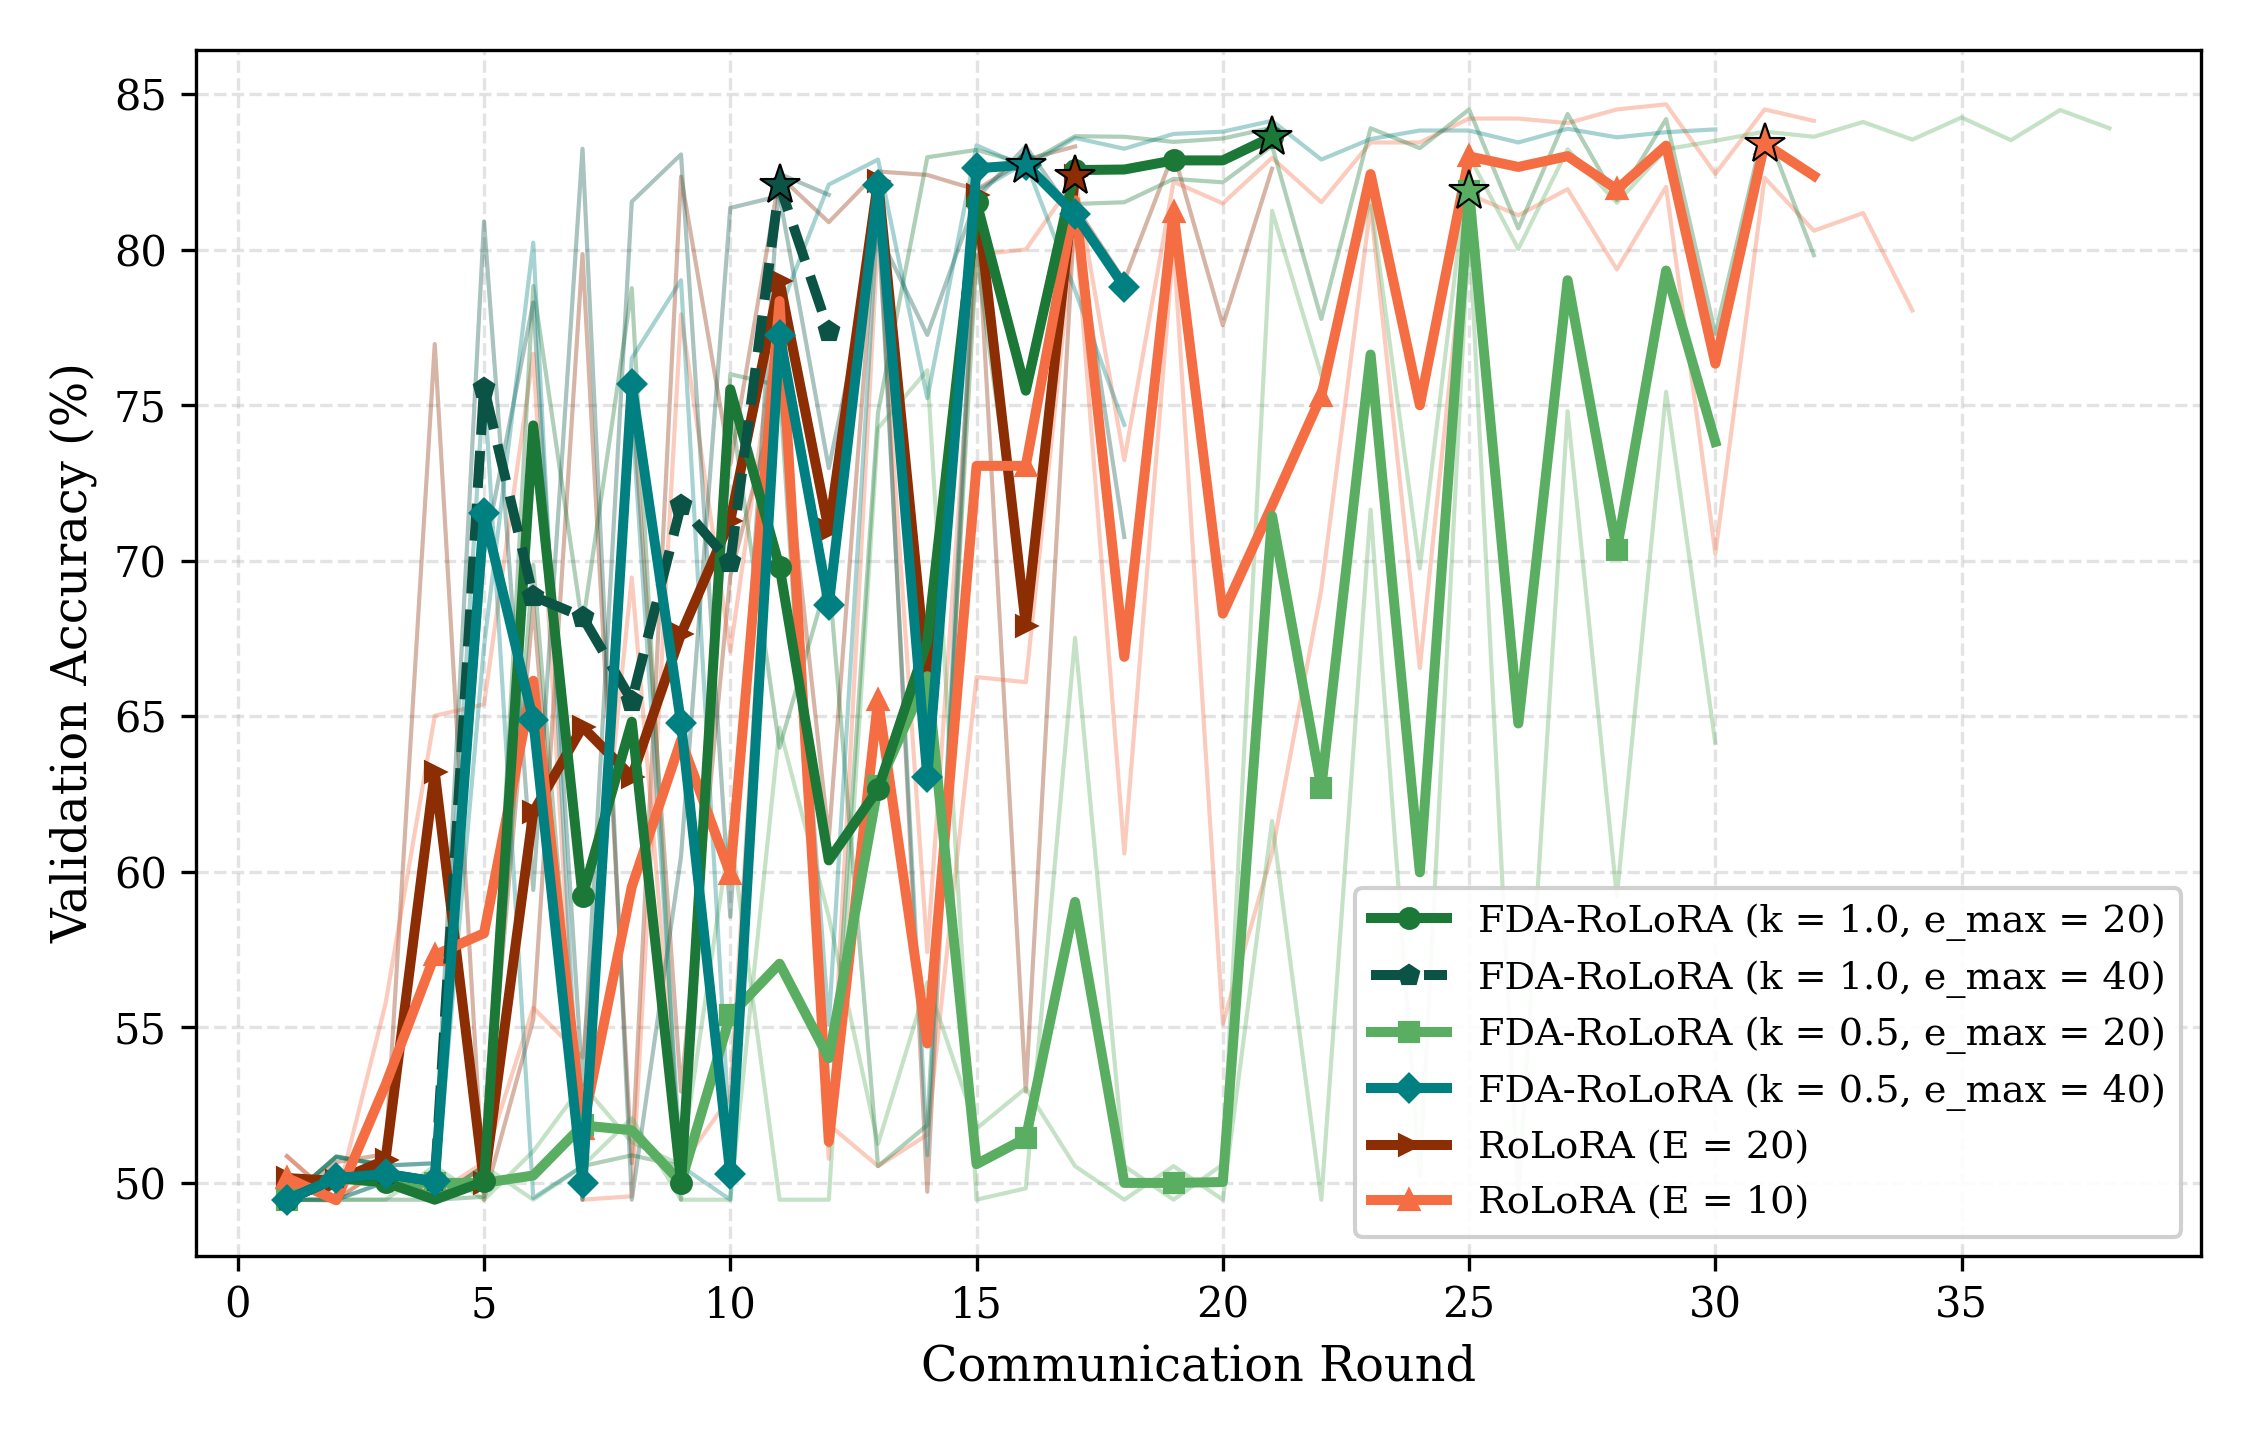
\includegraphics[width=\linewidth,height=0.62\textheight,keepaspectratio]{figures/18_QNLI_C20_R50_LR0.1_A0.5_1_accuracy.png}
            \vspace{-0.2em}
            \tiny \textbf{Figure}: Validation accuracy vs.\ communication rounds on QNLI under Dirichlet skew ($\alpha=0.5, C=20$).
        \end{column}
    \end{columns}
\end{frame}

\begin{frame}{Evaluation : Stability: Peak Accuracy Overstates the Benefit}
    \vspace{-0.3em}
    \begin{block}{Disparity Between Peak and Final Convergence}
        \small
        \begin{itemize}
            \item 13 of 38 Non-IID FDA-RoLoRA runs ended at least 10 points below their peak, compared with 3 of 20 RoLoRA runs.
            \item Under IID data: 2 of 32 FDA-RoLoRA runs and 2 of 46 RoLoRA runs.
            \item SST-2 ($C = 20, k = 1.0$): one seed fell from $89.3\%$ to $49.1\%$.
            \item QNLI ($C = 50$): both FDA-RoLoRA variants ended near chance.
            \item QQP ($C = 20$): final accuracy $64.52\%$ for FDA-RoLoRA vs.\ $76.76\%$ for RoLoRA $E = 10$.
            \item \textbf{Exception}: on SST-2 ($C = 50$), FDA-RoLoRA ended above RoLoRA in both seeds.
        \end{itemize}
    \end{block}
\end{frame}

\begin{frame}{Evaluation : Rounds and Data to Reach Accuracy Gates}
    \framesubtitle{Non-IID ($\alpha = 0.5$), FDA-RoLoRA with $k = 1.0$}
    \vspace{-0.4em}
    \centering
    \resizebox{0.95\textwidth}{!}{%
    \renewcommand{\arraystretch}{0.95}
    \begin{tabular}{lcccc}
        \toprule
        \textbf{Gate} & \textbf{RoLoRA $E=10$} & \textbf{RoLoRA $E=20$} & \textbf{FDA adapter MB} & \textbf{FDA with sketches} \\
        \midrule
        MNLI ($C=20$) $\ge 65\%$ & $131.2\,\text{MB}$ ($28$ rd) & $70.3\,\text{MB}$ ($15$ rd) & $84.4\,\text{MB}$ ($18$ rd) & $116.3\,\text{MB}$ \\
        MNLI ($C=20$) $\ge 70\%$ & $164.1\,\text{MB}$ ($35$ rd) & $86.8\,\text{MB}$ ($18.5$ rd) & $107.8\,\text{MB}$ ($23$ rd) & $150.4\,\text{MB}$ \\
        MNLI ($C=20$) final accuracy ($73.17\% / 74.25\%$) & $227.3\,\text{MB}$ ($48.5$ rd) & Fell to $68.87\%$ & $178.1\,\text{MB}$ ($38$ rd) & $254.2\,\text{MB}$ \\
        SST-2 ($C=20$) $\ge 85\%$ & $64.7\,\text{MB}$ ($23$ rd) & Not run & $23.9\,\text{MB}$ ($8.5$ rd) & $35.2\,\text{MB}$ \\
        \bottomrule
    \end{tabular}%
    }
    
    \vspace{0.2em}
    {\tiny \textit{Table Note}: Adapter MB excludes monitoring. Sketch figures add $6\,\text{KB}$ per client per epoch and assume the same training trajectory.}
    
    \vspace{0.35em}
    \begin{columns}[t]
        \begin{column}{0.48\textwidth}
            \begin{exampleblock}{Faster Than E = 10}
                \scriptsize
                FDA-RoLoRA reaches the MNLI gates in fewer rounds than $E = 10$, and reaches final accuracy in 13--30\% fewer rounds. $E = 20$ reaches the $65\%$ and $70\%$ gates sooner, then falls to $68.87\%$. On SST-2 ($C = 20$), it reaches $85\%$ in $8.5$ vs.\ $23$ rounds, but one seed later fell to $49\%$.
            \end{exampleblock}
        \end{column}
        \begin{column}{0.48\textwidth}
            \begin{exampleblock}{SST-2 (C = 50) Plateau Escape}
                \scriptsize
                RoLoRA $E = 10$ stays near the majority-class baseline (final $51.15\%$ and $55.50\%$). FDA-RoLoRA ends at $88.42\%$ and $74.31\%$ within the same 20 rounds. One of two seeds reached $85\%$.
            \end{exampleblock}
        \end{column}
    \end{columns}
\end{frame}

\begin{frame}{Evaluation : Monitoring Cost: What the MB Figures Exclude}
    \vspace{-0.3em}
    \centering
    \resizebox{0.92\textwidth}{!}{%
    \renewcommand{\arraystretch}{1.05}
    \begin{tabular}{lcc}
        \toprule
        \textbf{Monitoring} & \textbf{Added cost on top of adapter MB} & \textbf{MNLI Non-IID total (RoLoRA $E=10$: $227.3\,\text{MB}$)} \\
        \midrule
        Not counted (thesis) & None & $178.1\,\text{MB}$ ($-22\%$) \\
        $6\,\text{KB}$ sketch per epoch & $+15\%$ to $+59\%$ & $254.2\,\text{MB}$ ($+12\%$) \\
        Exact upload per epoch & $3.5\times$ to $9.2\times$ & $1{,}645\,\text{MB}$ ($7.2\times$) \\
        \bottomrule
    \end{tabular}%
    }
    
    \vspace{0.8em}
    \begin{block}{Impact of Monitoring Overhead}
        \small
        \begin{itemize}
            \item Correction: the 2.5--5.8\% overhead in the thesis assumes one check per round, but FDA-RoLoRA checks every epoch.
            \item Break-even with $6\,\text{KB}$ sketches: about $20\%$ fewer rounds at $\bar{e} = 10$, and about $30\%$ at $\bar{e} = 17.5$, at equal accuracy.
            \item Sketch figures assume the same training trajectory. No real sketch run was performed.
        \end{itemize}
    \end{block}
\end{frame}


% ==============================================================================
% SECTION 5: Conclusion & Future Work
% ==============================================================================
\section{Conclusion \& Future Work}

\begin{frame}{Conclusion : Synthesis of Scientific Contributions}
    \vspace{-0.3em}
    \framesubtitle{Core Theoretical and Empirical Insights from FDA-RoLoRA}
    \vspace{-0.3em}
    \scriptsize
    \begin{itemize}
        \item \textbf{Preservation of Aggregation Linearity}:
        \begin{itemize}
            \scriptsize
            \item Updating both adapter matrices simultaneously incurs bilinear aggregation error ($\frac{1}{N}\sum B_i A_i \neq \bar{B}\bar{A}$), distorting client updates and misguiding variance tracking.
            \item Alternating coordinate optimization isolates one factor ($A$ or $B$) per round, maintaining strictly linear updates and enabling stable geometric drift measurement.
        \end{itemize}
        \vspace{0.1em}
        \item \textbf{Scale-Decoupled Geometric Monitoring}:
        \begin{itemize}
            \scriptsize
            \item Tracking variance directly on low-rank coordinate tensors avoids the memory cost of full-model estimation. Its communication cost was not measured.
            \item Decoupled factor thresholds ($\theta_A, \theta_B$) resolve coordinate scale disparity while preserving symmetrical local epoch progression ($\bar{e}_A \approx \bar{e}_B$).
        \end{itemize}
        \vspace{0.1em}
        \item \textbf{Empirical Foundation Model Benchmarks (\texttt{roberta-base}, 173 Runs)}:
        \begin{itemize}
            \scriptsize
            \item \textbf{Non-IID Label Skew ($\alpha=0.5$)}: Controller tracks setpoint closely ($\mathcal{S} \approx 0.91\text{--}1.11$); reaches target accuracy in 13--30\% fewer rounds on MNLI ($C=20$) and escapes the majority plateau on SST-2 ($C=50$, $+26.95\%$).
            \item \textbf{IID Consensus ($\alpha=1000$)}: Controller undershoots the target epoch setpoint ($\mathcal{S} \approx 0.64\text{--}0.79$); demonstrates no consistent communication advantage over fixed-epoch RoLoRA.
            \item \textbf{Communication}: Round savings were observed, but a byte saving against RoLoRA is not established.
            \item \textbf{Stability}: Several non-IID runs lost accuracy late, so peak accuracy overstates the benefit.
        \end{itemize}
    \end{itemize}
\end{frame}
\begin{frame}{Conclusion : Limitations \& Future Research Horizons}
    \begin{columns}
        \begin{column}{0.49\textwidth}
            \begin{block}{Practical \& Experimental Limitations}
                \scriptsize
                \begin{itemize}
                    \item \textbf{RoLoRA Reimplementation}: Original codebase unavailable; reimplemented inside FDA-Opt framework.
                    \item \textbf{Hyperparameter Search}: RoLoRA paper omitted key LRs; required extensive empirical tuning.
                    \item \textbf{Compute Constraints}: Evaluated on \texttt{roberta-base} (125M); multi-billion LLMs remain future targets.
                    \item \textbf{Simulated FL}: Multi-process on 2$\times$A10 GPUs; real WAN latency and dropouts unmodeled.
                    \item \textbf{Monitoring Cost}: Per-epoch monitoring communication was not measured, and real sketches were not run.
                \end{itemize}
            \end{block}
        \end{column}
        \begin{column}{0.49\textwidth}
            \begin{block}{Future Research Horizons}
                \scriptsize
                \begin{itemize}
                    \item \textbf{Larger Foundation Models}: Scale to autoregressive LLMs (LLaMA, Mistral) on instruction-tuning.
                    \item \textbf{Broader PEFT Integration}: Synthesize FDA with SLoRA, FFA-LoRA, and dynamic rank (AdaLoRA).
                    \item \textbf{Partial Participation}: Evaluate under subsampled client cohorts and alternative factor alternation orders.
                    \item \textbf{Ecosystem Integration}: Upstream native FDA-RoLoRA support into FederatedScope-LLM.
                    \item \textbf{Monitoring Evaluation}: Run FDA-RoLoRA with real AMS sketches and LinearFDA, and measure total communication.
                \end{itemize}
            \end{block}
        \end{column}
    \end{columns}
\end{frame}
\begin{frame}{Key References}
    \scriptsize
    \begin{thebibliography}{99}
        \bibitem{chen2025robust}
        S.~Chen, Y.~Guo, Y.~Ju, H.~Dalal, Z.~Zhu, and A.~Khisti.
        \newblock \textbf{Robust Federated Finetuning of LLMs via Alternating Optimization of LoRA}.
        \newblock In \emph{Advances in Neural Information Processing Systems (NeurIPS)}, 2025.
        
        \bibitem{theologitis2025edbt}
        M.~Theologitis, V.~Samoladas, and A.~Deligiannakis.
        \newblock \textbf{Dynamic Averaging in Federated Learning}.
        \newblock In \emph{Proc. 28th International Conference on Extending Database Technology (EDBT)}, 2025.
        
        \bibitem{theologitis2025fdaopt}
        M.~Theologitis, V.~Samoladas, and A.~Deligiannakis.
        \newblock \textbf{FDA-Opt: Communication-Efficient Federated Fine-Tuning of Language Models}.
        \newblock \emph{arXiv preprint arXiv:2505.04535}, 2025.
        
        \bibitem{yang2025federated}
        H.~Yang, Y.~Wang, J.~Zhang, T.~Lu, S.~Vahidian, et~al.
        \newblock \textbf{Federated Low-Rank Adaptation for Foundation Models: A Survey}.
        \newblock In \emph{Proc. 34th Int. Joint Conf. on Artificial Intelligence (IJCAI)}, Survey Track, 2025.
        
        \bibitem{hu2022lora}
        E.~J.~Hu, Y.~Shen, P.~Wallis, Z.~Allen-Zhu, Y.~Li, S.~Wang, L.~Wang, and W.~Chen.
        \newblock \textbf{LoRA: Low-Rank Adaptation of Large Language Models}.
        \newblock In \emph{International Conference on Learning Representations (ICLR)}, 2022.
    \end{thebibliography}
\end{frame}
\begin{frame}[label=thank_you]
    \centering
    \Huge \textbf{Thank You!}
    
    \vspace{0.8em}
    \Large Questions \& Discussion
    
    \vspace{1.2em}
    \normalsize
    Asterinos Karalis -- \href{https://www.tuc.gr/}{\textbf{\color{tucblue}Technical University of Crete}}\\[0.2em]
    \href{https://www.ece.tuc.gr/}{\small \color{tucgray}School of Electrical \& Computer Engineering}\\
    \vspace{0.4em}
    \small Open-Source Repository: \url{https://github.com/Asterinos1/FDA-RoLoRA}
    
    \vspace{1.2em}
    {\scriptsize \color{tucgray} \textbf{Backup Slides (Q\&A Quick Jump):}}\\[0.25em]
    \hyperlink{backup_algo}{\beamerbutton{Algorithm \& Early Stop}} \quad
    \hyperlink{backup_testbed}{\beamerbutton{Hardware \& Testbed}} \quad
    \hyperlink{backup_threshold_evolution}{\beamerbutton{Threshold Evolution}} \quad
    \hyperlink{backup_factor_asymmetry}{\beamerbutton{Factor Asymmetry}} \\[0.25em]
    \hyperlink{backup_noniid_mnli}{\beamerbutton{MNLI Non-IID Plots}} \quad
    \hyperlink{backup_noniid_table}{\beamerbutton{Full Non-IID Table}} \quad
    \hyperlink{backup_iid_table}{\beamerbutton{Full IID Table}} \quad
    \hyperlink{backup_iid_mnli_qnli}{\beamerbutton{IID Plots (1)}} \quad
    \hyperlink{backup_iid_qqp_sst2}{\beamerbutton{IID Plots (2)}}
\end{frame}

% ==============================================================================
% APPENDIX / BACKUP SLIDES (Hidden from Total Slide Count & Table of Contents)
% ==============================================================================
\appendix

\begin{frame}[noframenumbering, label=backup_algo]{Backup : FDA-RoLoRA Algorithm \& Early-Stopping Harness}
    \framesubtitle{Complete Pseudocode (Algorithm 3) \& Simulation Control Parameters \hfill \hyperlink{main_impl}{\beamerreturnbutton{Back to Setup}} \; \hyperlink{thank_you}{\beamerreturnbutton{Q\&A}}}
    \vspace{-0.55em}
    \tiny
    \begin{columns}[t]
        \begin{column}{0.52\textwidth}
            \begin{block}{Algorithm 3: FDA-RoLoRA Execution Loop}
                \begin{enumerate}
                    \item \textbf{Init}: $W = W_0 + \frac{\alpha}{r} B_0 A_0$; $\theta_A = \theta_B = 0$; decoupled server optimizers for $A$ and $B$.
                    \item \textbf{For} round $r = 0, 1, 2, \dots$:
                    \begin{itemize}
                        \tiny
                        \item Toggle active matrix $\mathcal{M}^{(r)} \in \{B, A\}$ ($B$ on even rounds, $A$ on odd).
                        \item Load active threshold $\theta_{\text{current}}^{(r)} \leftarrow \theta_{\mathcal{M}^{(r)}}$ and broadcast $W_{\text{act}}^{(r)}$.
                        \item \textbf{For} local epoch $e = 1 \dots e_{\max}$:
                        \begin{itemize}
                            \tiny
                            \item Each client $i \in S_r$ steps $W_{i,e}^{(r)} \leftarrow W_{i,e-1}^{(r)} - \eta_c \nabla \mathcal{L}_i$ and computes $\Delta_i^{(e)} = W_{i,e}^{(r)} - W_{\text{act}}^{(r)}$.
                            \item \textbf{If} $e \ge e_{\min}$ and ($\text{Var}_{\text{subspace}}(\Delta^{(e)}) > \theta_{\text{current}}^{(r)}$ or $e = e_{\max}$): set $e^* \leftarrow e$ and \textbf{break}.
                        \end{itemize}
                        \item Server computes $\nabla_{\text{pseudo}}^{(r)} = -\frac{1}{|S_r|}\sum_{i \in S_r} \Delta_i^{(e^*)}$ and updates $W_{\text{act}}^{(r+1)}$.
                        \item Update active threshold $\theta_{\mathcal{M}^{(r)}} \leftarrow \left(\frac{k \cdot e_{\max}}{e^*}\right)\text{Var}_{\text{subspace}}(\Delta^{(e^*)})$ (dormant track frozen).
                    \end{itemize}
                \end{enumerate}
            \end{block}
        \end{column}
        \begin{column}{0.45\textwidth}
            \begin{block}{Accuracy-Gated Early Stopping (Sec. 4.3)}
                \begin{itemize}
                    \item \textbf{Sliding-Window Smoothing ($W$)}: Trailing moving average over $W=3$ (IID) or $W=5$ (Non-IID) rounds to filter stochastic non-IID oscillations.
                    \item \textbf{Accuracy Activation Gate ($A_{\text{gate}}$)}: Disarmed during initial coordinate calibration until validation accuracy crosses task milestone.
                    \item \textbf{Patience ($P$) \& Min Gain ($\Delta_{\min}$)}: Terminates if smoothed accuracy fails to improve by $\Delta_{\min} = 0.5\%$ over $P \in \{3, 5\}$ rounds.
                    \item \textbf{Mandatory Round Guard ($R_{\min}$)}: Enforces minimum alternating cycles before any stop trigger.
                \end{itemize}
            \end{block}
        \end{column}
    \end{columns}
    \vspace{0.2em}\par{\tiny \textit{Note}: Variance is exact in simulation; monitoring communication is not counted.}
\end{frame}

\begin{frame}[noframenumbering, label=backup_testbed]{Backup : Testbed Implementation \& Hardware Environment}
    \framesubtitle{Physical Infrastructure, Execution Orchestration \& Client Constraints \hfill \hyperlink{main_impl}{\beamerreturnbutton{Back to Setup}} \; \hyperlink{thank_you}{\beamerreturnbutton{Q\&A}}}
    \footnotesize
    \begin{columns}[t]
        \begin{column}{0.48\textwidth}
            \begin{block}{Polytechnix Server Testbed}
                \begin{itemize}
                    \item \textbf{Server}: SoftNet Lab Polytechnix GPU server.
                    \item \textbf{GPUs}: $2\times$ NVIDIA Ampere A10 ($24\,\text{GB}$ VRAM each).
                    \item \textbf{CPUs}: $2\times$ Intel Xeon Silver 4310 ($24\text{c}/48\text{t}$, $2.10\,\text{GHz}$).
                    \item \textbf{RAM}: $256\,\text{GB}$ DDR4 system memory.
                    \item \textbf{Comparability}: All 173 runs evaluated exclusively on this uniform platform to ensure perfect comparability.
                \end{itemize}
            \end{block}
        \end{column}
        \begin{column}{0.48\textwidth}
            \begin{block}{Simulation Pipeline Orchestration}
                \begin{itemize}
                    \item \textbf{Alternation}: Track $B$ on even rounds ($t=0,2,\dots$), Track $A$ on odd rounds ($t=1,3,\dots$).
                    \item \textbf{Client Simulation}: Sequential in-silico GPU client simulation (constraining VRAM to one active client) paired with 6 concurrent jobs ($3$/GPU) across $2\times$ A10 GPUs.
                    \item \textbf{Batch Sizes}: $B = 32$ (MNLI, QNLI, QQP), $B = 64$ (SST-2, following Chen et al., 2025).
                    \item \textbf{Client Partitions}: Dirichlet-sampled private data splits with frozen backbone weights.
                \end{itemize}
            \end{block}
        \end{column}
    \end{columns}
\end{frame}

\begin{frame}[noframenumbering, label=backup_threshold_evolution]{Backup : Threshold Evolution \& Design Explorations}
    \framesubtitle{Generalized Proportional Setpoint Control Law \& Pilot Decisions \hfill \hyperlink{thank_you}{\beamerreturnbutton{Q\&A}}}
    \vspace{-0.65em}
    \begin{block}{Generalized Proportional Setpoint Control Law}
        \scriptsize
        Active threshold scales proportionally to realized epoch $e^*$ relative to target setpoint $k \cdot e_{\max}$ ($k \in (0, 1]$), while dormant track remains frozen:
        $$\theta_{\mathcal{M}^{(r)}}^{(\text{next})} = \left( \frac{k \cdot e_{\max}}{e^*} \right) \text{Var}_{\text{subspace}}(\Delta^{(e^*)}) \quad \text{where } k=0.5 \implies \frac{e_{\max}}{2} \text{ (Midpoint)}, \; k=1.0 \implies e_{\max} \text{ (Ceiling)}$$
        \begin{itemize}
            \item \textbf{Self-Stabilizing Feedback}: Early halt ($e^* < k e_{\max}$) expands $\theta$ next cycle; late halt ($e^* > k e_{\max}$) tightens $\theta$.
        \end{itemize}
    \end{block}
    \vspace{-0.5em}
    \begin{block}{Evolutionary Design Decisions (Explored \& Discarded in Pilot Study)}
        \scriptsize
        \begin{itemize}
            \item \textbf{Simultaneous FDA + FedLoRA}: Suffered bilinear product error ($\frac{1}{N}\sum B_i A_i \neq \bar{B}\bar{A}$) $\to$ premature accuracy plateaus.
            \item \textbf{Dense Reconstruction (FDA-LoRA-SVD)}: Server-side truncated SVD on $\sum B_i A_i$ restored accuracy, but $\mathcal{O}(d^2)$ communication and $\mathcal{O}(d^2 r)$ SVD latency proved prohibitive.
            \item \textbf{Single Shared Threshold ($\theta$)}: Cross-matrix scale contamination ($\theta_B \gg \theta_A$) caused erratic halting across tracks.
            \item \textbf{Temporal Smoothing (EMA / SMA)}: Introduced phase lag across alternating subspaces; memoryless feedback proved superior.
        \end{itemize}
    \end{block}
\end{frame}

\begin{frame}[noframenumbering, label=backup_factor_asymmetry]{Backup : Factor Asymmetry \& Decoupled Tracking}
    \framesubtitle{Local Epoch Symmetry ($\bar{e}_A \approx \bar{e}_B$) \& Threshold Decoupling \hfill \hyperlink{thank_you}{\beamerreturnbutton{Q\&A}}}
    \begin{columns}
        \begin{column}{0.46\textwidth}
            \begin{block}{Scale Disparity, Not Deeper Training}
                \scriptsize
                \begin{itemize}
                    \item \textbf{Down-Projection} $A$: Gaussian initialization.
                    \item \textbf{Up-Projection} $B$: Zero initialization ($\Delta W = 0$).
                    \item Initialization induces severe numerical scale disparity ($\theta_B \gg \theta_A$).
                    \item Decoupled thresholds $(\theta_A, \theta_B)$ are essential to prevent a shared threshold from choking $A$ or over-training $B$.
                \end{itemize}
            \end{block}
            
            \begin{exampleblock}{Empirical Symmetry}
                \scriptsize
                Across all Non-IID benchmarks (Table 5.2), decoupled thresholds yield remarkably \textbf{symmetrical} epoch progression across factors ($\bar{e}_A \approx \bar{e}_B$).
            \end{exampleblock}
        \end{column}
        
        \begin{column}{0.52\textwidth}
            \centering
            \resizebox{\columnwidth}{!}{%
            \begin{tabular}{lcccccc}
                \toprule
                \textbf{Non-IID Setting ($\alpha=0.5$)} & $\mathbf{e_{\max}}$ & $\mathbf{k}$ & $\mathbf{e^*}$ & $\mathbf{\bar{e}}$ & $\mathbf{\mathcal{S}}$ & $\mathbf{\bar{e}_A \;/\; \bar{e}_B}$ \\
                \midrule
                MNLI ($C=20$)  & 20 & 0.50 & 10.0 & $10.07$ & 1.01 & $9.96 \;/\; 10.18$ \\
                MNLI ($C=20$)  & 20 & 1.00 & 20.0 & $17.49$ & 0.87 & $17.19 \;/\; 17.76$ \\
                MNLI ($C=20$)  & 40 & 0.50 & 20.0 & $19.06$ & 0.95 & $18.82 \;/\; 19.29$ \\
                QNLI ($C=20$)  & 20 & 1.00 & 20.0 & $16.73$ & 0.84 & $16.63 \;/\; 16.81$ \\
                QNLI ($C=20$)  & 40 & 1.00 & 40.0 & $29.83$ & 0.75 & $30.14 \;/\; 29.53$ \\
                SST-2 ($C=50$) & 20 & 1.00 & 20.0 & $14.57$ & 0.73 & $14.60 \;/\; 14.55$ \\
                \bottomrule
            \end{tabular}%
            }
            \vspace{0.4em}
            
            \begin{block}{Aggregate Regime Tracking Fidelity}
                \scriptsize
                Across steady-state horizons, Non-IID achieves high setpoint tracking ($\mathcal{S} = 1.11 \pm 0.08$ at $k=0.5$; $\mathcal{S} = 0.91 \pm 0.05$ at $k=1.0$), whereas IID undershoots ($\mathcal{S} = 0.79$ at $k=0.5$; $\mathcal{S} = 0.64$ at $k=1.0$).
            \end{block}
        \end{column}
    \end{columns}
\end{frame}

\begin{frame}[noframenumbering, label=backup_noniid_mnli]{Backup : MNLI Non-IID Plots \& Epoch Dynamics}
    \framesubtitle{Dirichlet Label Skew ($\alpha=0.5, C=20$): 6-Panel Plots \& Setpoint Tracking \hfill \hyperlink{main_noniid}{\beamerreturnbutton{Back to Non-IID}} \; \hyperlink{thank_you}{\beamerreturnbutton{Q\&A}}}
    \vspace{-0.5em}
    \begin{columns}[c]
        \begin{column}{0.49\textwidth}
            \centering
            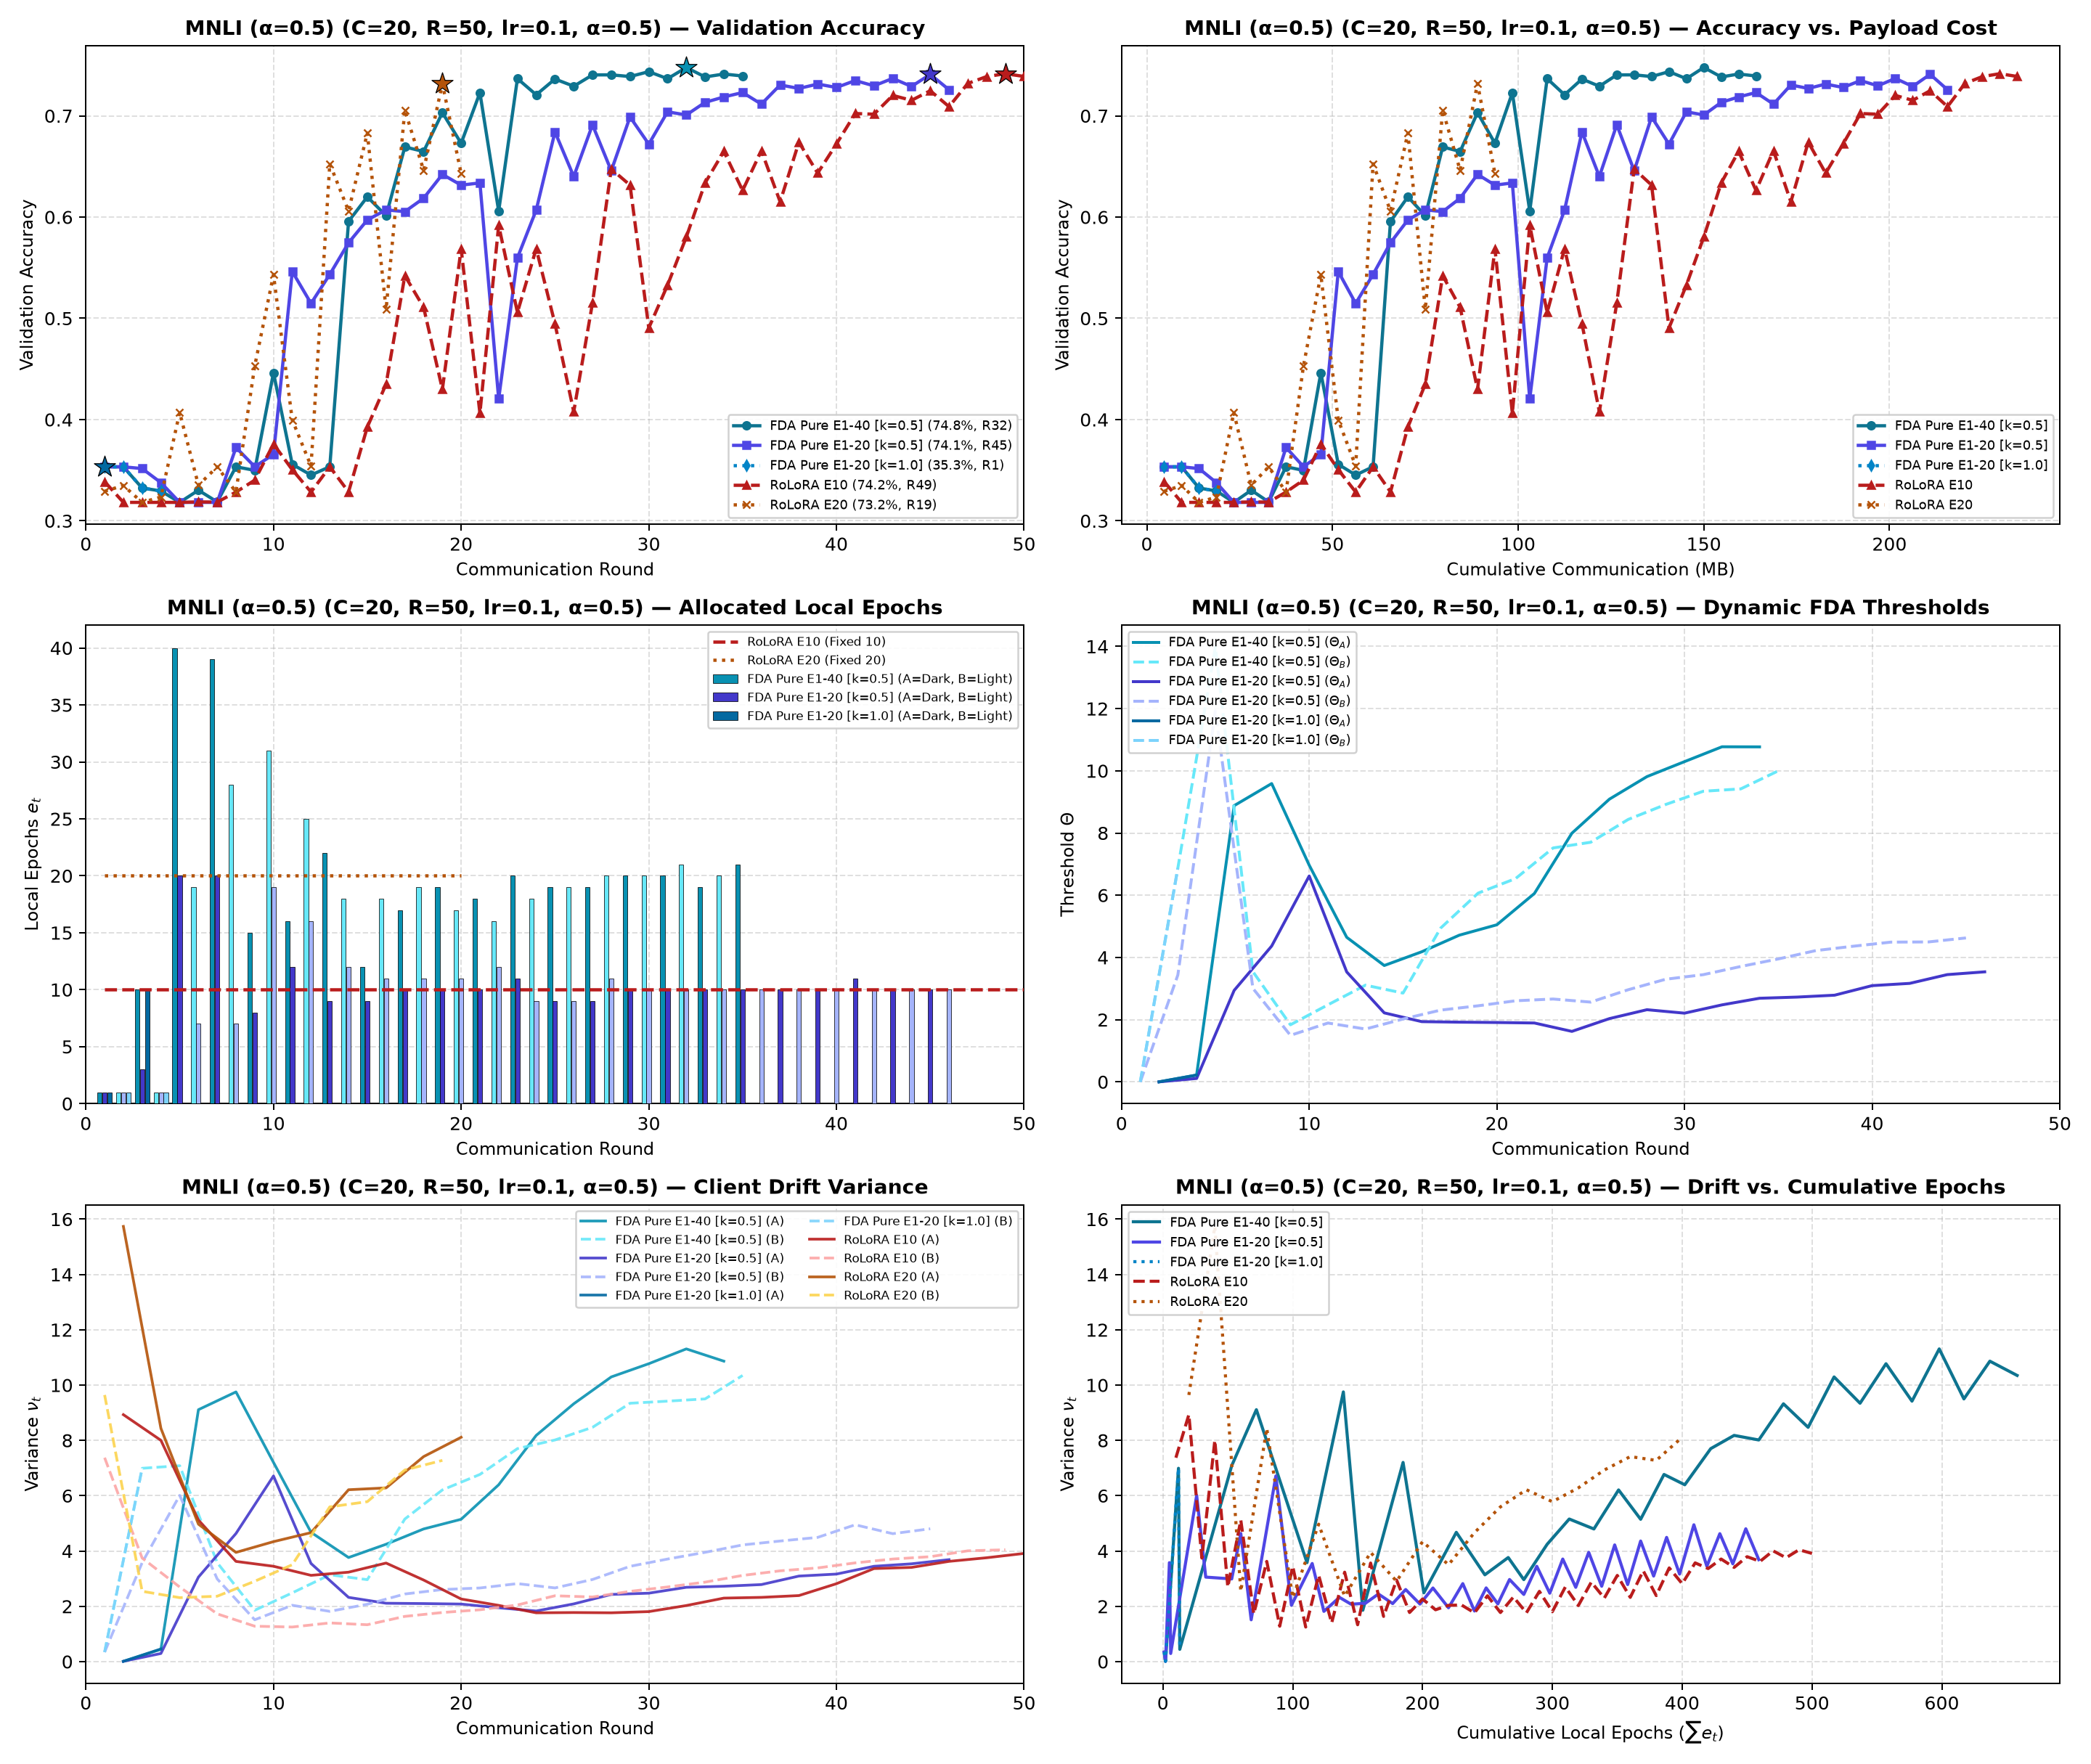
\includegraphics[width=\textwidth,height=0.58\textheight,keepaspectratio]{figures/17_MNLI_C20_R50_LR0.1_A0.5_all6_telemetry_stacked.png}\\[-0.1em]
            {\tiny \textbf{Fig. 5.9}: MNLI Non-IID ($C=20$): FDA-RoLoRA reaches $74.47\%$ peak and reaches final accuracy in 13--30\% fewer rounds than RoLoRA $E = 10$, while RoLoRA $E=20$ collapses ($73.31\% \to 68.87\%$).}
        \end{column}
        \begin{column}{0.49\textwidth}
            \centering
            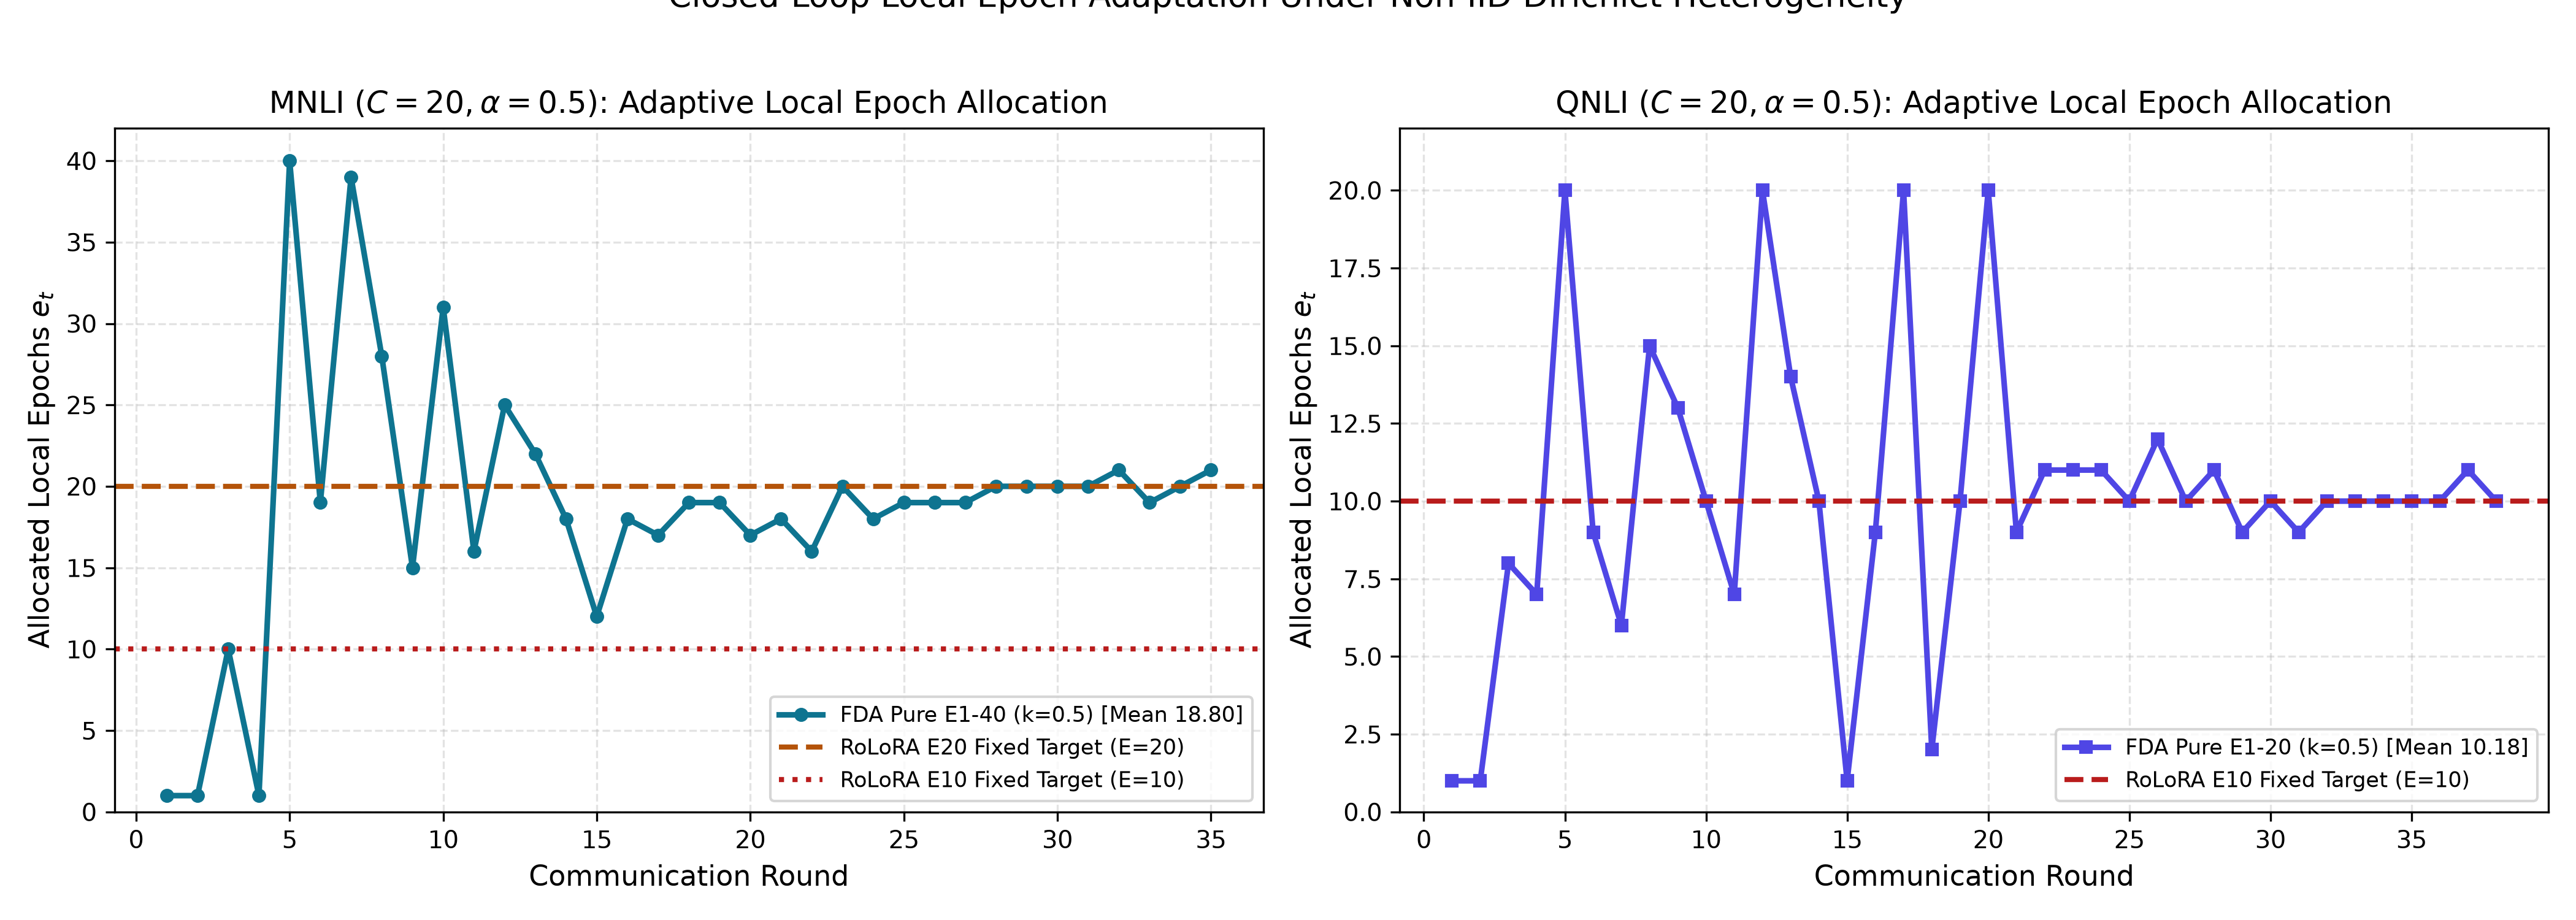
\includegraphics[width=0.92\textwidth,height=0.27\textheight,keepaspectratio]{figures/non_iid_epoch_dynamics.png}\\[0.15em]
            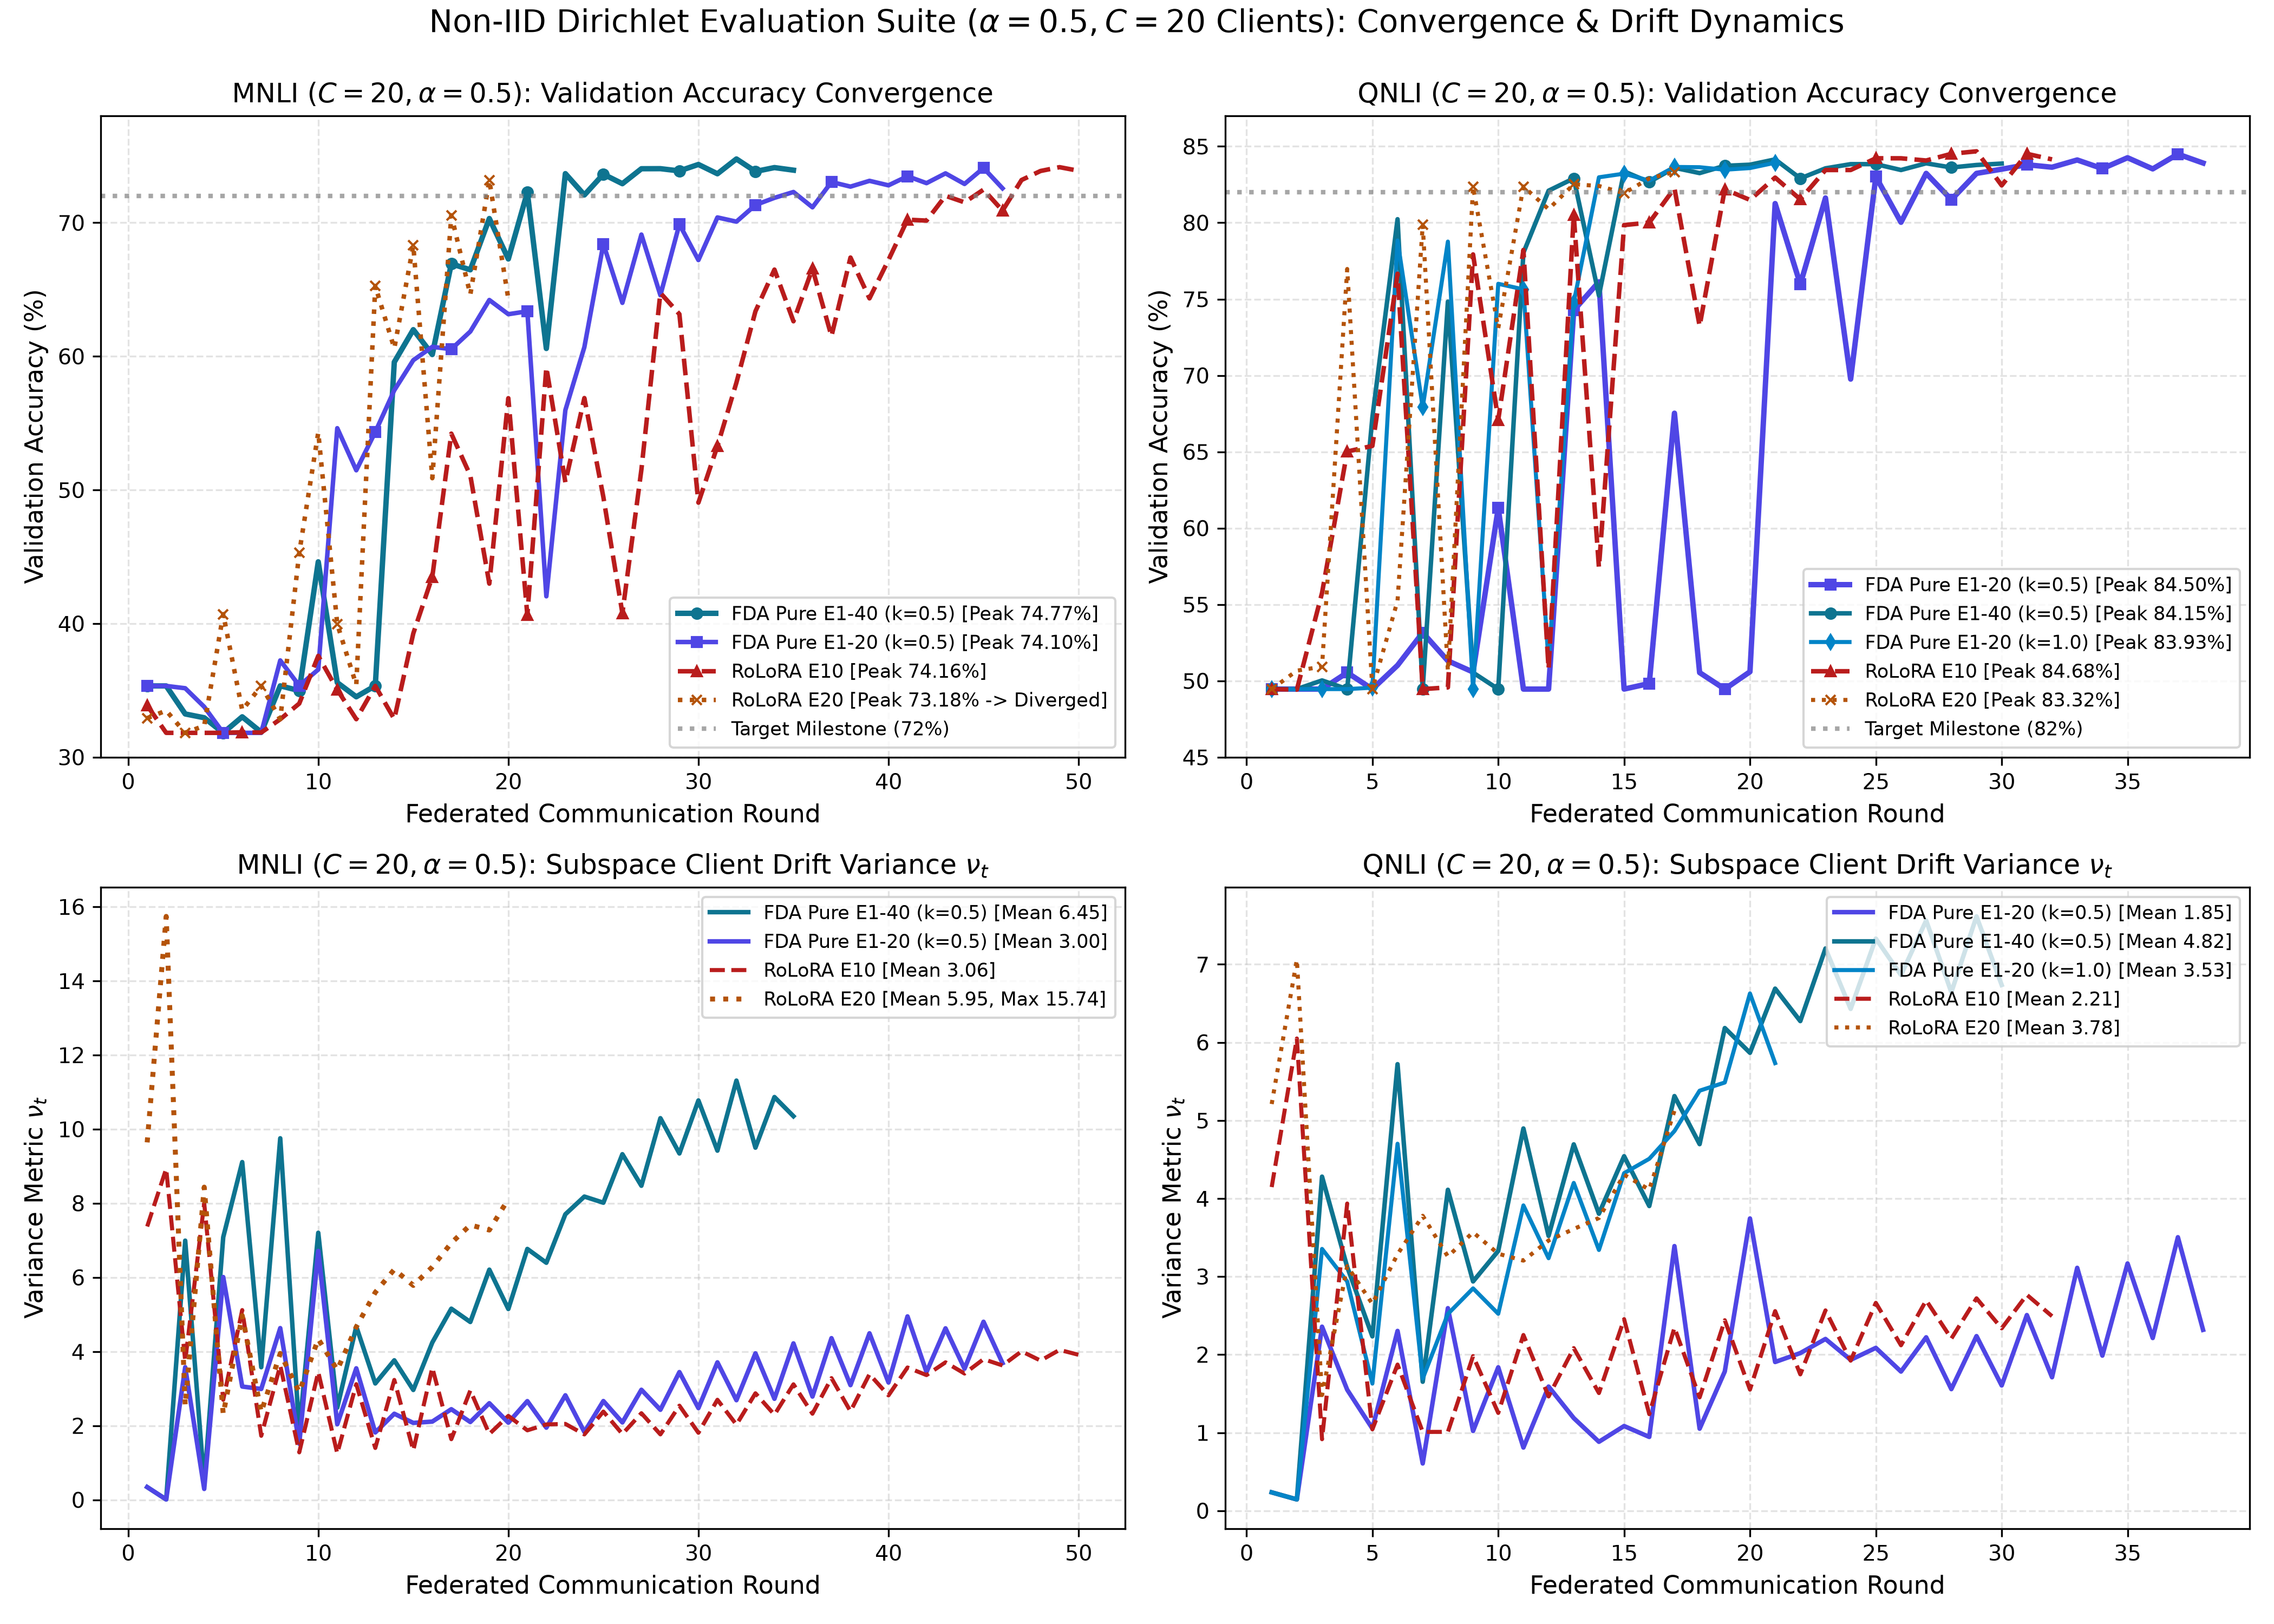
\includegraphics[width=0.92\textwidth,height=0.27\textheight,keepaspectratio]{figures/non_iid_benchmark_telemetry.png}\\[-0.1em]
            {\tiny \textbf{Figs. 5.11 \& 5.12}: Top: Realized local epochs per round hovering around $k \cdot e_{\max}$ on MNLI ($e_{\max}=40, k=0.5$) and QNLI ($e_{\max}=20, k=0.5$). Bottom: Accuracy and coordinate drift variance $\sigma_t^2$.}
        \end{column}
    \end{columns}
\end{frame}

\begin{frame}[noframenumbering, label=backup_noniid_table]{Backup : Complete Non-IID Benchmark Table (Table 5.2)}
    \framesubtitle{All Evaluated Non-IID Configurations ($\alpha=0.5$) Across GLUE Benchmarks \hfill \hyperlink{main_scorecard}{\beamerreturnbutton{Back to Results Summary}} \; \hyperlink{thank_you}{\beamerreturnbutton{Q\&A}}}
    \vspace{-0.5em}
    \centering
    \resizebox{0.92\textwidth}{!}{%
    \renewcommand{\arraystretch}{0.82}
    \begin{tabular}{lllccccccc}
        \toprule
        \textbf{Task} & \textbf{Cohort} & \textbf{Methodology} & \textbf{Final Acc. (\%)} & \textbf{Peak Acc. (\%)} & \textbf{Rounds ($R$)} & \textbf{Total MB} & \textbf{Mean $\bar{e}$} & \textbf{Mean $\bar{e}_A$} & \textbf{Mean $\bar{e}_B$} \\
        \midrule
        \multirow{8}{*}{\textbf{MNLI}} 
        & \multirow{5}{*}{$C=20$ ($R_{\max}=50$)} 
        & FDA-RoLoRA E1TO40 ($k=0.5$) & $73.70 \pm 0.34$ & $74.12 \pm 0.93$ & $34.5 \pm 0.7$ & $161.7\,\text{MB}$ & $19.06$ & $18.82$ & $19.29$ \\
        & & FDA-RoLoRA E1TO20 ($k=0.5$) & $72.48 \pm 0.14$ & $73.25 \pm 1.19$ & $41.0 \pm 7.1$ & $192.2\,\text{MB}$ & $10.07$ & $9.96$ & $10.18$ \\
        & & FDA-RoLoRA E1TO20 ($k=1.0$) & $73.71 \pm 0.77$ & $\mathbf{74.47 \pm 0.11}$ & $38.0 \pm 4.2$ & $178.1\,\text{MB}$ & $17.49$ & $17.19$ & $17.76$ \\
        & & RoLoRA E20 & $68.87 \pm 6.46$ & $73.31 \pm 0.18$ & $\mathbf{24.0 \pm 5.7}$ & $\mathbf{112.5\,\text{MB}}$ & $20.00$ & $20.00$ & $20.00$ \\
        & & RoLoRA E10 & $\mathbf{74.11 \pm 0.31}$ & $74.24 \pm 0.12$ & $50.0$ & $234.4\,\text{MB}$ & $10.00$ & $10.00$ & $10.00$ \\
        \cmidrule{2-10}
        & \multirow{3}{*}{$C=50$ ($R_{\max}=30$)} 
        & FDA-RoLoRA E1TO20 ($k=1.0$) & $51.46 \pm 8.46$ & $54.95 \pm 3.53$ & $\mathbf{22.5 \pm 2.1}$ & $\mathbf{263.7\,\text{MB}}$ & $15.63$ & $15.03$ & $16.20$ \\
        & & FDA-RoLoRA E1TO20 ($k=0.5$) & $55.23 \pm 2.11$ & $55.56 \pm 1.65$ & $30.0$ & $351.6\,\text{MB}$ & $10.13$ & $9.47$ & $10.80$ \\
        & & RoLoRA E10 & $\mathbf{56.22 \pm 7.40}$ & $\mathbf{56.55 \pm 6.94}$ & $30.0$ & $351.6\,\text{MB}$ & $10.00$ & $10.00$ & $10.00$ \\
        \midrule
        \multirow{9}{*}{\textbf{QNLI}} 
        & \multirow{6}{*}{$C=20$ ($R_{\max}=50$)} 
        & FDA-RoLoRA E1TO40 ($k=1.0$) & $76.27 \pm 7.78$ & $83.20 \pm 0.18$ & $\mathbf{15.0 \pm 4.2}$ & $\mathbf{70.3\,\text{MB}}$ & $29.83$ & $30.14$ & $29.53$ \\
        & & FDA-RoLoRA E1TO40 ($k=0.5$) & $79.12 \pm 6.72$ & $83.48 \pm 0.94$ & $24.0 \pm 8.5$ & $112.5\,\text{MB}$ & $20.36$ & $21.24$ & $19.47$ \\
        & & FDA-RoLoRA E1TO20 ($k=1.0$) & $81.88 \pm 2.90$ & $\mathbf{84.22 \pm 0.41}$ & $26.5 \pm 7.8$ & $124.2\,\text{MB}$ & $16.73$ & $16.63$ & $16.81$ \\
        & & FDA-RoLoRA E1TO20 ($k=0.5$) & $74.03 \pm 13.98$ & $82.64 \pm 2.63$ & $34.0 \pm 5.7$ & $159.4\,\text{MB}$ & $10.54$ & $10.81$ & $10.27$ \\
        & & RoLoRA E20 & $\mathbf{82.97 \pm 0.50}$ & $83.22 \pm 0.14$ & $19.0 \pm 2.8$ & $89.1\,\text{MB}$ & $20.00$ & $20.00$ & $20.00$ \\
        & & RoLoRA E10 & $81.10 \pm 4.31$ & $83.50 \pm 1.67$ & $33.0 \pm 1.4$ & $154.7\,\text{MB}$ & $10.00$ & $10.00$ & $10.00$ \\
        \cmidrule{2-10}
        & \multirow{3}{*}{$C=50$ ($R_{\max}=30$)} 
        & FDA-RoLoRA E1TO20 ($k=1.0$) & $49.51 \pm 0.08$ & $73.52 \pm 4.31$ & $\mathbf{13.0}$ & $\mathbf{152.3\,\text{MB}}$ & $13.04$ & $13.17$ & $12.93$ \\
        & & FDA-RoLoRA E1TO20 ($k=0.5$) & $50.13 \pm 0.94$ & $\mathbf{75.69 \pm 1.66}$ & $30.0$ & $351.6\,\text{MB}$ & $10.48$ & $9.83$ & $11.13$ \\
        & & RoLoRA E10 & $\mathbf{58.45 \pm 12.71}$ & $74.61 \pm 10.15$ & $30.0$ & $351.6\,\text{MB}$ & $10.00$ & $10.00$ & $10.00$ \\
        \midrule
        \multirow{6}{*}{\textbf{QQP}} 
        & \multirow{3}{*}{$C=20$ ($R_{\max}=20$)} 
        & FDA-RoLoRA E1TO20 ($k=1.0$) & $64.52 \pm 18.23$ & $\mathbf{77.88 \pm 0.66}$ & $14.0 \pm 2.8$ & $65.6\,\text{MB}$ & $15.70$ & $15.77$ & $15.62$ \\
        & & FDA-RoLoRA E1TO20 ($k=0.5$) & $48.32 \pm 12.63$ & $73.58 \pm 1.56$ & $\mathbf{12.0 \pm 4.2}$ & $\mathbf{56.2\,\text{MB}}$ & $10.87$ & $11.79$ & $10.10$ \\
        & & RoLoRA E10 & $\mathbf{76.76 \pm 3.41}$ & $77.69 \pm 2.18$ & $16.5 \pm 0.7$ & $77.3\,\text{MB}$ & $10.00$ & $10.00$ & $10.00$ \\
        \cmidrule{2-10}
        & \multirow{3}{*}{$C=50$ ($R_{\max}=24$)} 
        & FDA-RoLoRA E1TO20 ($k=1.0$) & $57.45 \pm 11.29$ & $74.55 \pm 1.30$ & $\mathbf{15.5 \pm 3.5}$ & $\mathbf{181.6\,\text{MB}}$ & $14.26$ & $13.83$ & $14.63$ \\
        & & FDA-RoLoRA E1TO20 ($k=0.5$) & $53.46 \pm 19.74$ & $72.71 \pm 3.23$ & $\mathbf{15.5 \pm 4.9}$ & $\mathbf{181.6\,\text{MB}}$ & $9.18$ & $8.89$ & $9.48$ \\
        & & RoLoRA E10 & $\mathbf{69.28 \pm 8.14}$ & $\mathbf{74.71 \pm 1.63}$ & $22.5 \pm 2.1$ & $263.7\,\text{MB}$ & $10.00$ & $10.00$ & $10.00$ \\
        \midrule
        \multirow{6}{*}{\textbf{SST-2}} 
        & \multirow{3}{*}{$C=20$ ($R_{\max}=25$)} 
        & FDA-RoLoRA E1TO20 ($k=1.0$) & $69.72 \pm 29.19$ & $\mathbf{89.91 \pm 0.81}$ & $\mathbf{14.0}$ & $\mathbf{39.4\,\text{MB}}$ & $14.43$ & $14.57$ & $14.29$ \\
        & & FDA-RoLoRA E1TO20 ($k=0.5$) & $79.36 \pm 16.38$ & $89.39 \pm 2.19$ & $16.0 \pm 2.8$ & $45.0\,\text{MB}$ & $9.69$ & $10.32$ & $9.06$ \\
        & & RoLoRA E10 & $\mathbf{89.62 \pm 1.87}$ & $89.62 \pm 1.87$ & $25.0$ & $70.3\,\text{MB}$ & $10.00$ & $10.00$ & $10.00$ \\
        \cmidrule{2-10}
        & \multirow{3}{*}{$C=50$ ($R_{\max}=20$)} 
        & FDA-RoLoRA E1TO20 ($k=1.0$) & $\mathbf{81.36 \pm 9.97}$ & $\mathbf{85.95 \pm 5.60}$ & $\mathbf{20.0}$ & $\mathbf{140.6\,\text{MB}}$ & $14.57$ & $14.60$ & $14.55$ \\
        & & FDA-RoLoRA E1TO20 ($k=0.5$) & $66.46 \pm 24.57$ & $67.37 \pm 23.27$ & $\mathbf{20.0}$ & $\mathbf{140.6\,\text{MB}}$ & $8.70$ & $8.40$ & $9.00$ \\
        & & RoLoRA E10 & $53.33 \pm 3.08$ & $59.00 \pm 11.11$ & $\mathbf{20.0}$ & $\mathbf{140.6\,\text{MB}}$ & $10.00$ & $10.00$ & $10.00$ \\
        \bottomrule
    \end{tabular}%
    }
\end{frame}

\begin{frame}[noframenumbering, label=backup_iid_table]{Backup : Complete IID Benchmark Table (Table 5.1)}
    \framesubtitle{All Evaluated IID Configurations ($\alpha=1000.0$) Across GLUE Benchmarks \hfill \hyperlink{main_scorecard}{\beamerreturnbutton{Back to Results Summary}} \; \hyperlink{thank_you}{\beamerreturnbutton{Q\&A}}}
    \vspace{-0.6em}
    \centering
    \resizebox{0.76\textwidth}{!}{%
    \renewcommand{\arraystretch}{0.72}
    \begin{tabular}{lllcccccc}
        \toprule
        \textbf{Task} & \textbf{Cohort} & \textbf{Methodology} & \textbf{Final Acc. (\%)} & \textbf{Peak Acc. (\%)} & \textbf{Rounds ($R$)} & \textbf{Total MB} & \textbf{Mean $\bar{e}$} & \textbf{Drift Var. ($\bar{\nu}$)} \\
        \midrule
        \multirow{10}{*}{\textbf{MNLI}} 
        & \multirow{6}{*}{$C=20$ ($R_{\max}=50$)} 
        & FDA-RoLoRA E1TO20 ($k=1.0$) & $\mathbf{76.86 \pm 0.10}$ & $\mathbf{76.86 \pm 0.10}$ & $32.0 \pm 4.2$ & $150.0\,\text{MB}$ & $13.42$ & $6.552$ \\
        & & FDA-RoLoRA E1TO20 ($k=0.5$) & $76.44 \pm 0.18$ & $76.45 \pm 0.17$ & $41.0 \pm 4.2$ & $192.2\,\text{MB}$ & $7.76$ & $2.957$ \\
        & & RoLoRA E20 & $75.98 \pm 0.58$ & $76.28 \pm 0.16$ & $\mathbf{22.0}$ & $\mathbf{103.1\,\text{MB}}$ & $20.00$ & $10.149$ \\
        & & RoLoRA E15 & $75.21 \pm 2.67$ & $75.34 \pm 2.86$ & $22.5 \pm 2.1$ & $105.5\,\text{MB}$ & $15.00$ & $6.004$ \\
        & & RoLoRA E10 & $76.60 \pm 0.85$ & $76.60 \pm 0.85$ & $28.0 \pm 1.4$ & $131.2\,\text{MB}$ & $10.00$ & $3.713$ \\
        & & RoLoRA E5 & $63.89 \pm 14.80$ & $68.52 \pm 8.25$ & $32.5 \pm 9.2$ & $152.3\,\text{MB}$ & $5.00$ & $0.711$ \\
        \cmidrule{2-9}
        & \multirow{4}{*}{$C=50$ ($R_{\max}=30$)} 
        & FDA-RoLoRA E1TO20 ($k=1.0$) & $\mathbf{69.85 \pm 3.37}$ & $\mathbf{69.85 \pm 3.37}$ & $\mathbf{30.0}$ & $\mathbf{351.6\,\text{MB}}$ & $12.15$ & $1.115$ \\
        & & FDA-RoLoRA E1TO20 ($k=0.5$) & $56.16 \pm 7.99$ & $56.16 \pm 7.99$ & $\mathbf{30.0}$ & $\mathbf{351.6\,\text{MB}}$ & $7.22$ & $0.106$ \\
        & & RoLoRA E10 & $65.85 \pm 2.85$ & $65.85 \pm 2.85$ & $\mathbf{30.0}$ & $\mathbf{351.6\,\text{MB}}$ & $10.00$ & $0.416$ \\
        & & RoLoRA E5 & $34.57 \pm 2.43$ & $35.81 \pm 0.67$ & $\mathbf{30.0}$ & $\mathbf{351.6\,\text{MB}}$ & $5.00$ & $0.010$ \\
        \midrule
        \multirow{9}{*}{\textbf{QNLI}} 
        & \multirow{4}{*}{$C=20$ ($R_{\max}=50$)} 
        & FDA-RoLoRA E1TO20 ($k=1.0$) & $67.63 \pm 22.28$ & $\mathbf{83.14 \pm 0.34}$ & $16.5 \pm 3.5$ & $77.3\,\text{MB}$ & $9.85$ & $1.111$ \\
        & & FDA-RoLoRA E1TO20 ($k=0.5$) & $65.28 \pm 22.37$ & $80.61 \pm 0.69$ & $17.5 \pm 0.7$ & $82.0\,\text{MB}$ & $6.91$ & $0.448$ \\
        & & RoLoRA E10 & $\mathbf{75.03 \pm 10.54}$ & $81.83 \pm 0.92$ & $\mathbf{10.0 \pm 1.4}$ & $\mathbf{46.9\,\text{MB}}$ & $10.00$ & $0.977$ \\
        & & RoLoRA E5 & $71.72 \pm 14.63$ & $81.79 \pm 0.39$ & $16.5 \pm 2.1$ & $77.3\,\text{MB}$ & $5.00$ & $0.373$ \\
        \cmidrule{2-9}
        & \multirow{5}{*}{$C=50$ ($R_{\max}=30$)} 
        & FDA-RoLoRA E1TO20 ($k=1.0$) & $82.47 \pm 1.72$ & $82.77 \pm 2.14$ & $\mathbf{21.0 \pm 5.7}$ & $\mathbf{246.1\,\text{MB}}$ & $10.89$ & $0.707$ \\
        & & FDA-RoLoRA E1TO20 ($k=0.5$) & $80.75 \pm 0.17$ & $80.96 \pm 0.18$ & $26.0 \pm 4.2$ & $304.7\,\text{MB}$ & $7.35$ & $0.213$ \\
        & & RoLoRA E20 & $\mathbf{87.94 \pm 0.00}$ & $\mathbf{88.14 \pm 0.00}$ & $30.0$ & $351.6\,\text{MB}$ & $20.00$ & $11.343$ \\
        & & RoLoRA E10 & $82.00 \pm 1.85$ & $82.85 \pm 1.61$ & $24.5 \pm 2.1$ & $287.1\,\text{MB}$ & $10.00$ & $0.435$ \\
        & & RoLoRA E5 & $78.82 \pm 1.48$ & $79.25 \pm 0.87$ & $30.0$ & $351.6\,\text{MB}$ & $5.00$ & $0.034$ \\
        \midrule
        \multirow{8}{*}{\textbf{QQP}} 
        & \multirow{4}{*}{$C=20$ ($R_{\max}=50$)} 
        & FDA-RoLoRA E1TO20 ($k=1.0$) & $\mathbf{76.34 \pm 5.33}$ & $\mathbf{78.57 \pm 4.23}$ & $17.5 \pm 6.4$ & $82.0\,\text{MB}$ & $10.69$ & $1.576$ \\
        & & FDA-RoLoRA E1TO20 ($k=0.5$) & $72.96 \pm 0.58$ & $74.17 \pm 1.12$ & $14.0 \pm 1.4$ & $65.6\,\text{MB}$ & $6.50$ & $0.543$ \\
        & & RoLoRA E10 & $75.47 \pm 1.19$ & $75.47 \pm 1.19$ & $\mathbf{6.5 \pm 0.7}$ & $\mathbf{30.5\,\text{MB}}$ & $10.00$ & $0.761$ \\
        & & RoLoRA E5 & $72.46 \pm 1.17$ & $73.58 \pm 0.20$ & $10.0$ & $46.9\,\text{MB}$ & $5.00$ & $0.323$ \\
        \cmidrule{2-9}
        & \multirow{4}{*}{$C=50$ ($R_{\max}=30$)} 
        & FDA-RoLoRA E1TO20 ($k=1.0$) & $72.65 \pm 1.17$ & $73.63 \pm 0.03$ & $\mathbf{14.0}$ & $\mathbf{164.1\,\text{MB}}$ & $9.14$ & $0.220$ \\
        & & FDA-RoLoRA E1TO20 ($k=0.5$) & $72.08 \pm 0.20$ & $73.86 \pm 0.39$ & $18.0 \pm 1.4$ & $210.9\,\text{MB}$ & $6.25$ & $0.206$ \\
        & & RoLoRA E10 & $\mathbf{75.43 \pm 1.07}$ & $\mathbf{78.79 \pm 1.38}$ & $30.0$ & $351.6\,\text{MB}$ & $10.00$ & $0.731$ \\
        & & RoLoRA E5 & $75.36 \pm 0.50$ & $75.36 \pm 0.50$ & $30.0$ & $351.6\,\text{MB}$ & $5.00$ & $0.221$ \\
        \midrule
        \multirow{10}{*}{\textbf{SST-2}} 
        & \multirow{5}{*}{$C=20$ ($R_{\max}=50$)} 
        & FDA-RoLoRA E1TO20 ($k=1.0$) & $91.80 \pm 0.24$ & $92.14 \pm 0.24$ & $20.5 \pm 0.7$ & $57.7\,\text{MB}$ & $11.11$ & $0.654$ \\
        & & FDA-RoLoRA E1TO20 ($k=0.5$) & $87.61 \pm 5.35$ & $88.88 \pm 3.73$ & $17.5 \pm 7.8$ & $49.2\,\text{MB}$ & $5.82$ & $0.113$ \\
        & & RoLoRA E20 & $\mathbf{92.16 \pm 0.13}$ & $\mathbf{92.55 \pm 0.30}$ & $\mathbf{10.7 \pm 1.5}$ & $\mathbf{30.0\,\text{MB}}$ & $20.00$ & $2.387$ \\
        & & RoLoRA E10 & $91.51 \pm 0.32$ & $91.80 \pm 0.08$ & $15.0 \pm 1.4$ & $42.2\,\text{MB}$ & $10.00$ & $0.327$ \\
        & & RoLoRA E5 & $90.31 \pm 1.22$ & $90.60 \pm 0.81$ & $21.0 \pm 1.4$ & $59.1\,\text{MB}$ & $5.00$ & $0.105$ \\
        \cmidrule{2-9}
        & \multirow{5}{*}{$C=50$ ($R_{\max}=30$)} 
        & FDA-RoLoRA E1TO20 ($k=1.0$) & $89.68 \pm 1.14$ & $89.68 \pm 1.14$ & $20.0 \pm 5.7$ & $140.6\,\text{MB}$ & $10.78$ & $0.063$ \\
        & & FDA-RoLoRA E1TO20 ($k=0.5$) & $86.81 \pm 4.05$ & $87.44 \pm 3.16$ & $25.0 \pm 7.1$ & $175.8\,\text{MB}$ & $6.91$ & $0.019$ \\
        & & RoLoRA E20 & $\mathbf{91.90 \pm 0.37}$ & $\mathbf{92.01 \pm 0.57}$ & $\mathbf{17.0 \pm 11.4}$ & $\mathbf{119.5\,\text{MB}}$ & $20.00$ & $1.660$ \\
        & & RoLoRA E10 & $89.91 \pm 0.49$ & $90.54 \pm 0.73$ & $22.0$ & $154.7\,\text{MB}$ & $10.00$ & $0.109$ \\
        & & RoLoRA E5 & $87.33 \pm 0.41$ & $87.50 \pm 0.65$ & $26.0 \pm 5.7$ & $182.8\,\text{MB}$ & $5.00$ & $0.013$ \\
        \bottomrule
    \end{tabular}%
    }
\end{frame}

\begin{frame}[noframenumbering, label=backup_iid_mnli_qnli]{Backup : Additional IID Plots (MNLI \& QNLI)}
    \framesubtitle{Multi-Panel Optimization Plots Under Homogeneous Consensus ($\alpha=1000.0$) \hfill \hyperlink{main_iid}{\beamerreturnbutton{Back to IID}} \; \hyperlink{thank_you}{\beamerreturnbutton{Q\&A}}}
    \vspace{-0.4em}
    \begin{columns}[c]
        \begin{column}{0.24\textwidth}
            \centering
            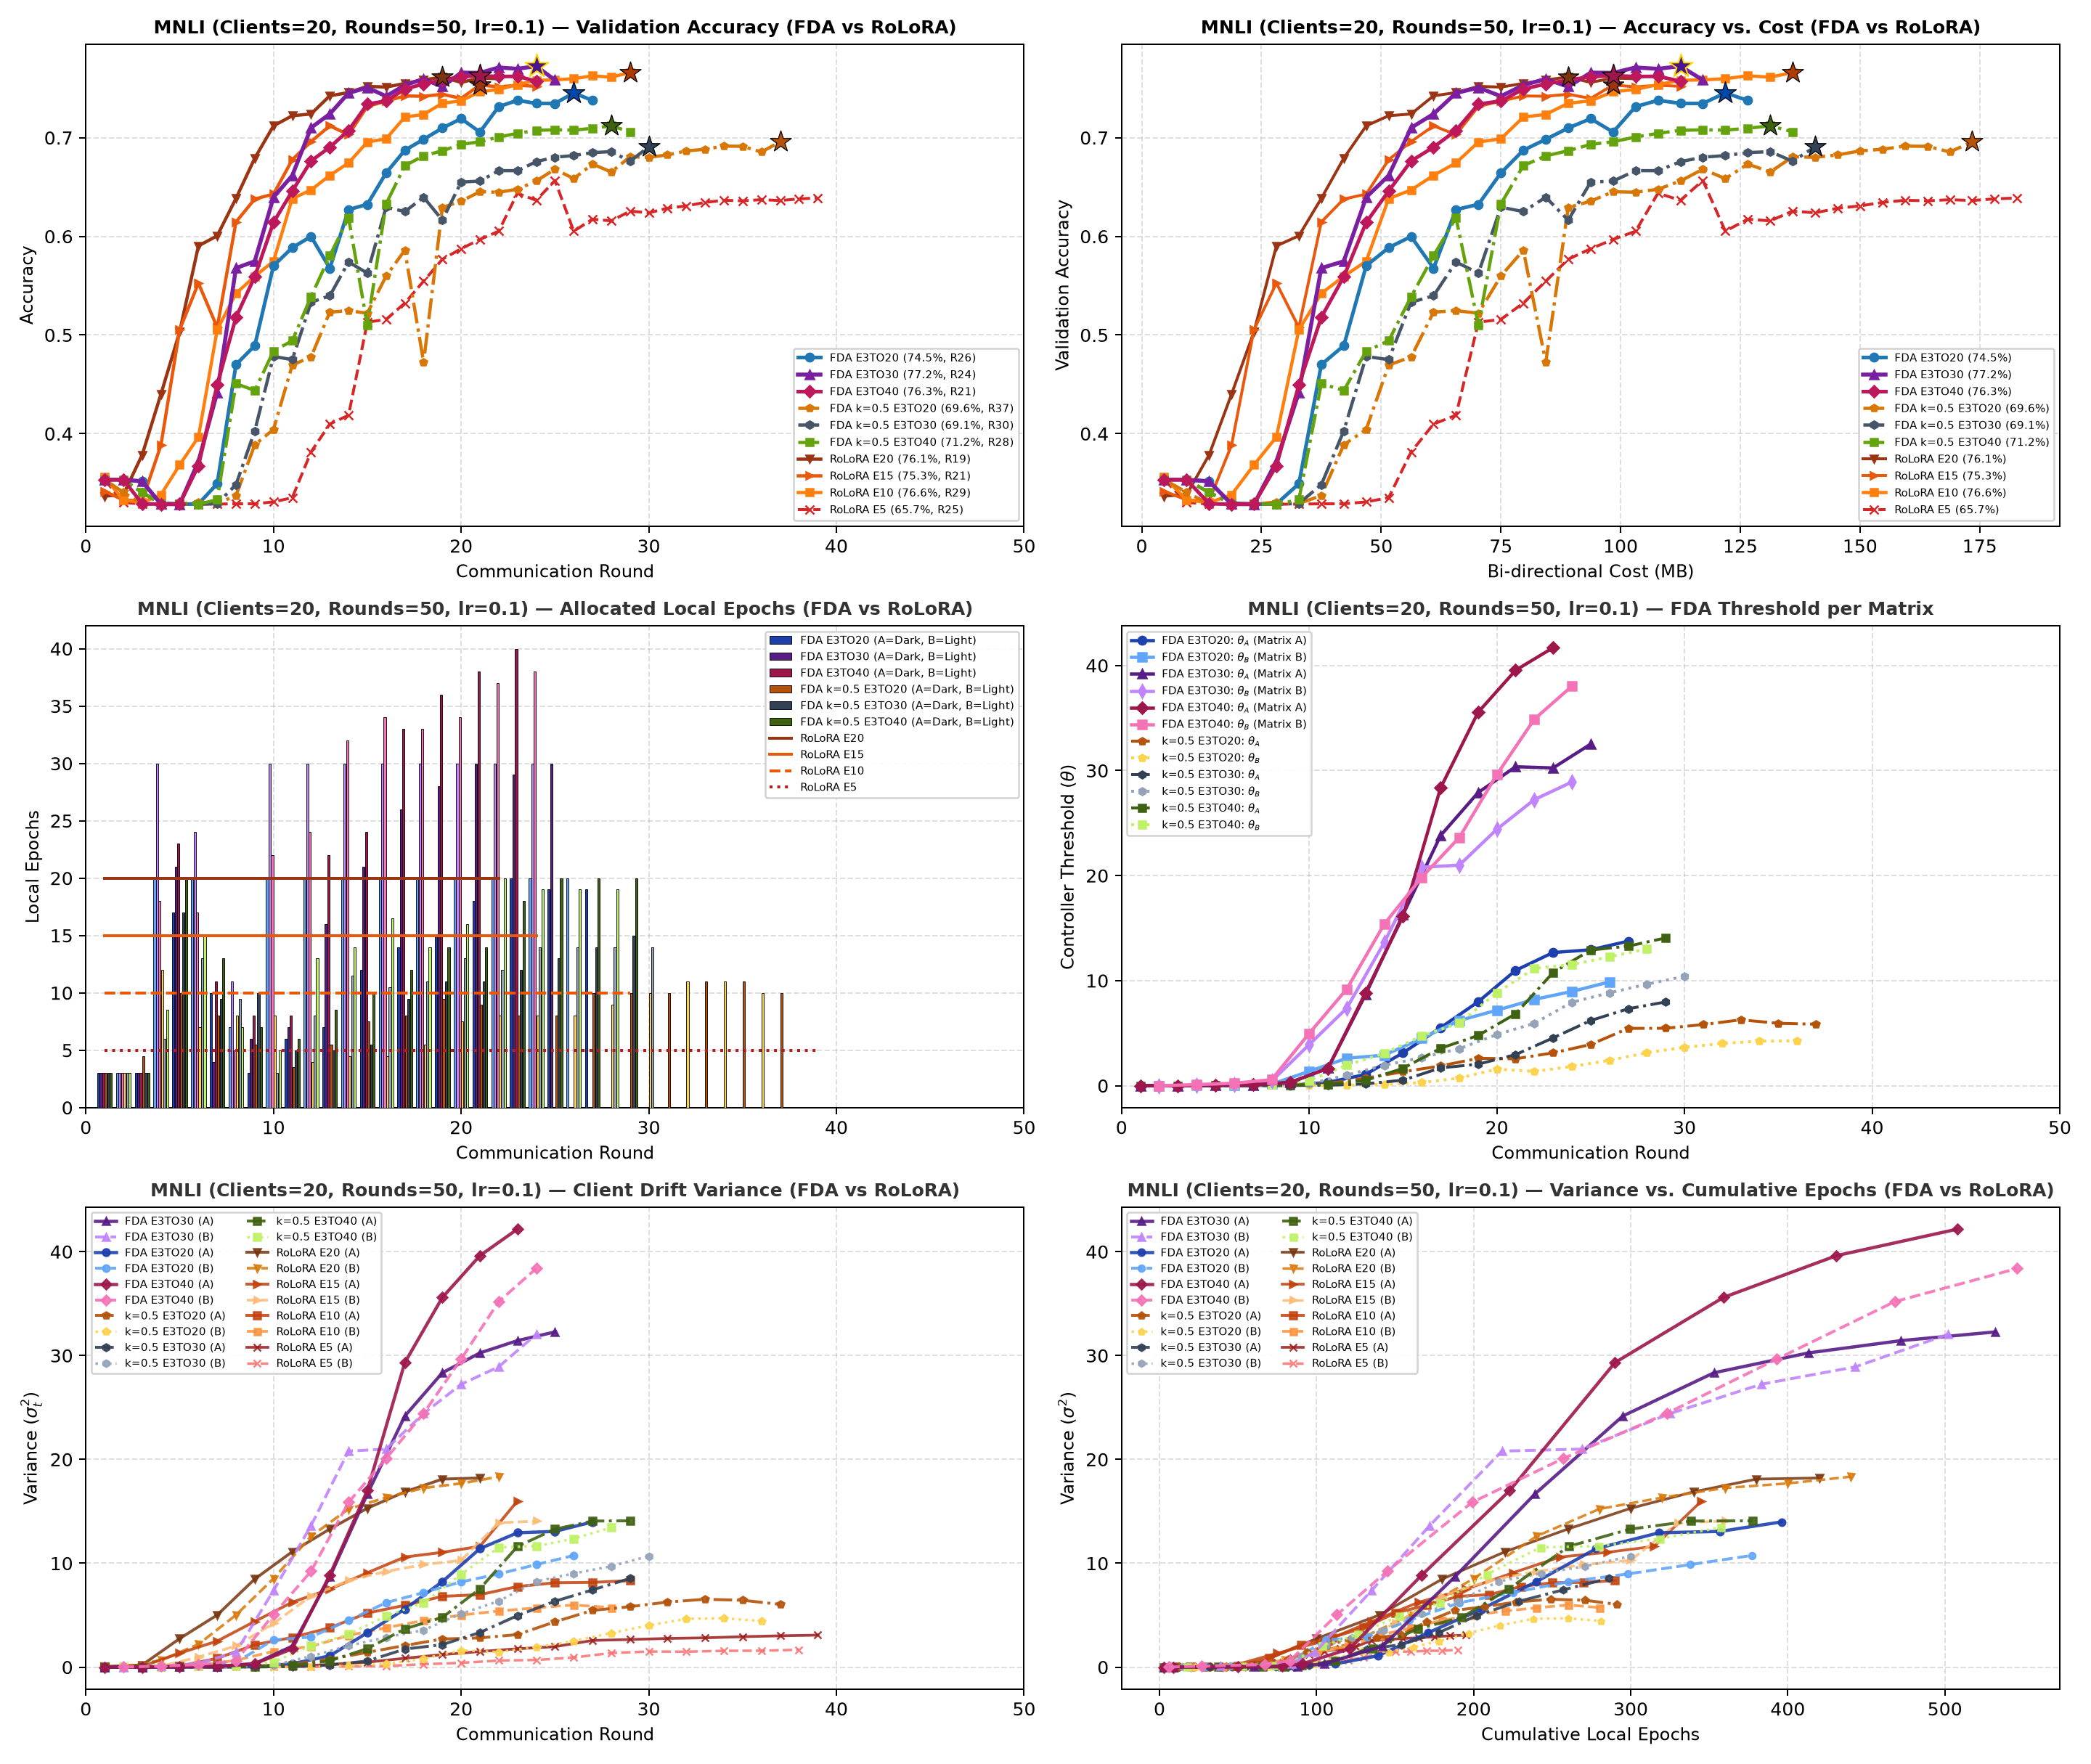
\includegraphics[width=\textwidth,height=0.62\textheight,keepaspectratio]{figures/01_MNLI_C20_R50_LR0.1_all6_telemetry_stacked.png}\\[-0.1em]
            {\tiny \textbf{MNLI ($C=20$, IID)}}
        \end{column}
        \begin{column}{0.24\textwidth}
            \centering
            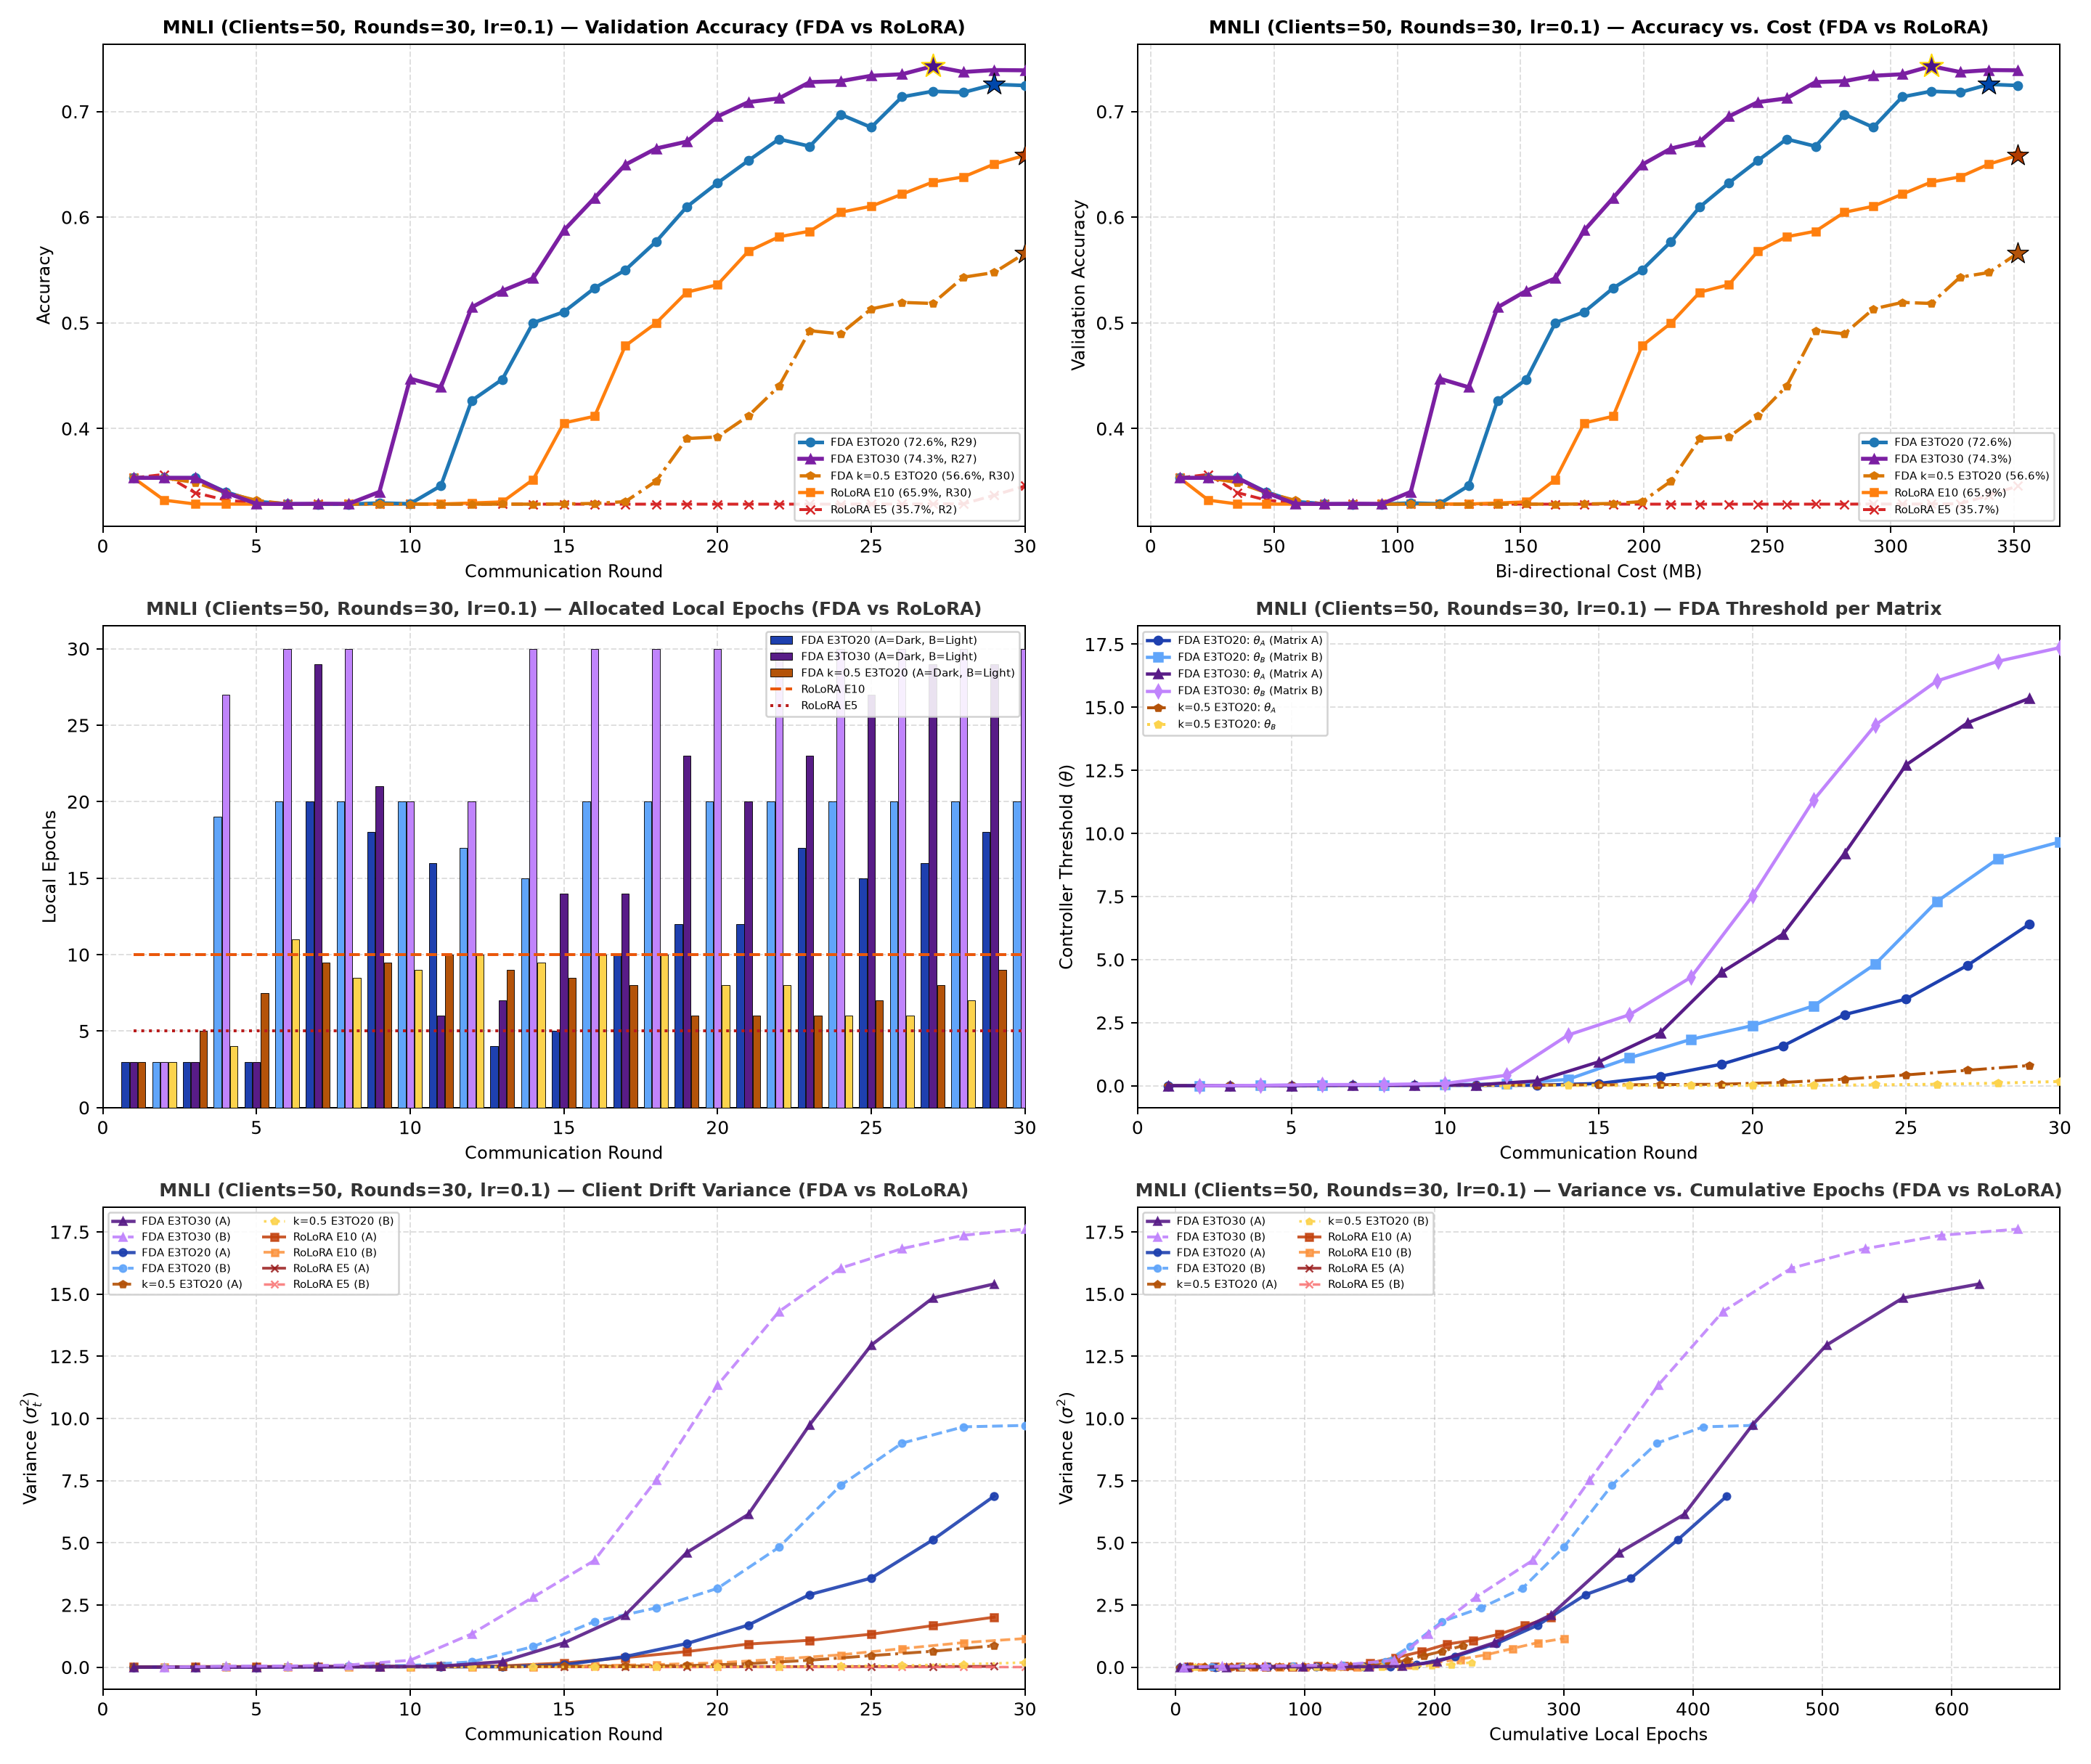
\includegraphics[width=\textwidth,height=0.62\textheight,keepaspectratio]{figures/03_MNLI_C50_R30_LR0.1_all6_telemetry_stacked.png}\\[-0.1em]
            {\tiny \textbf{MNLI ($C=50$, IID)}}
        \end{column}
        \begin{column}{0.24\textwidth}
            \centering
            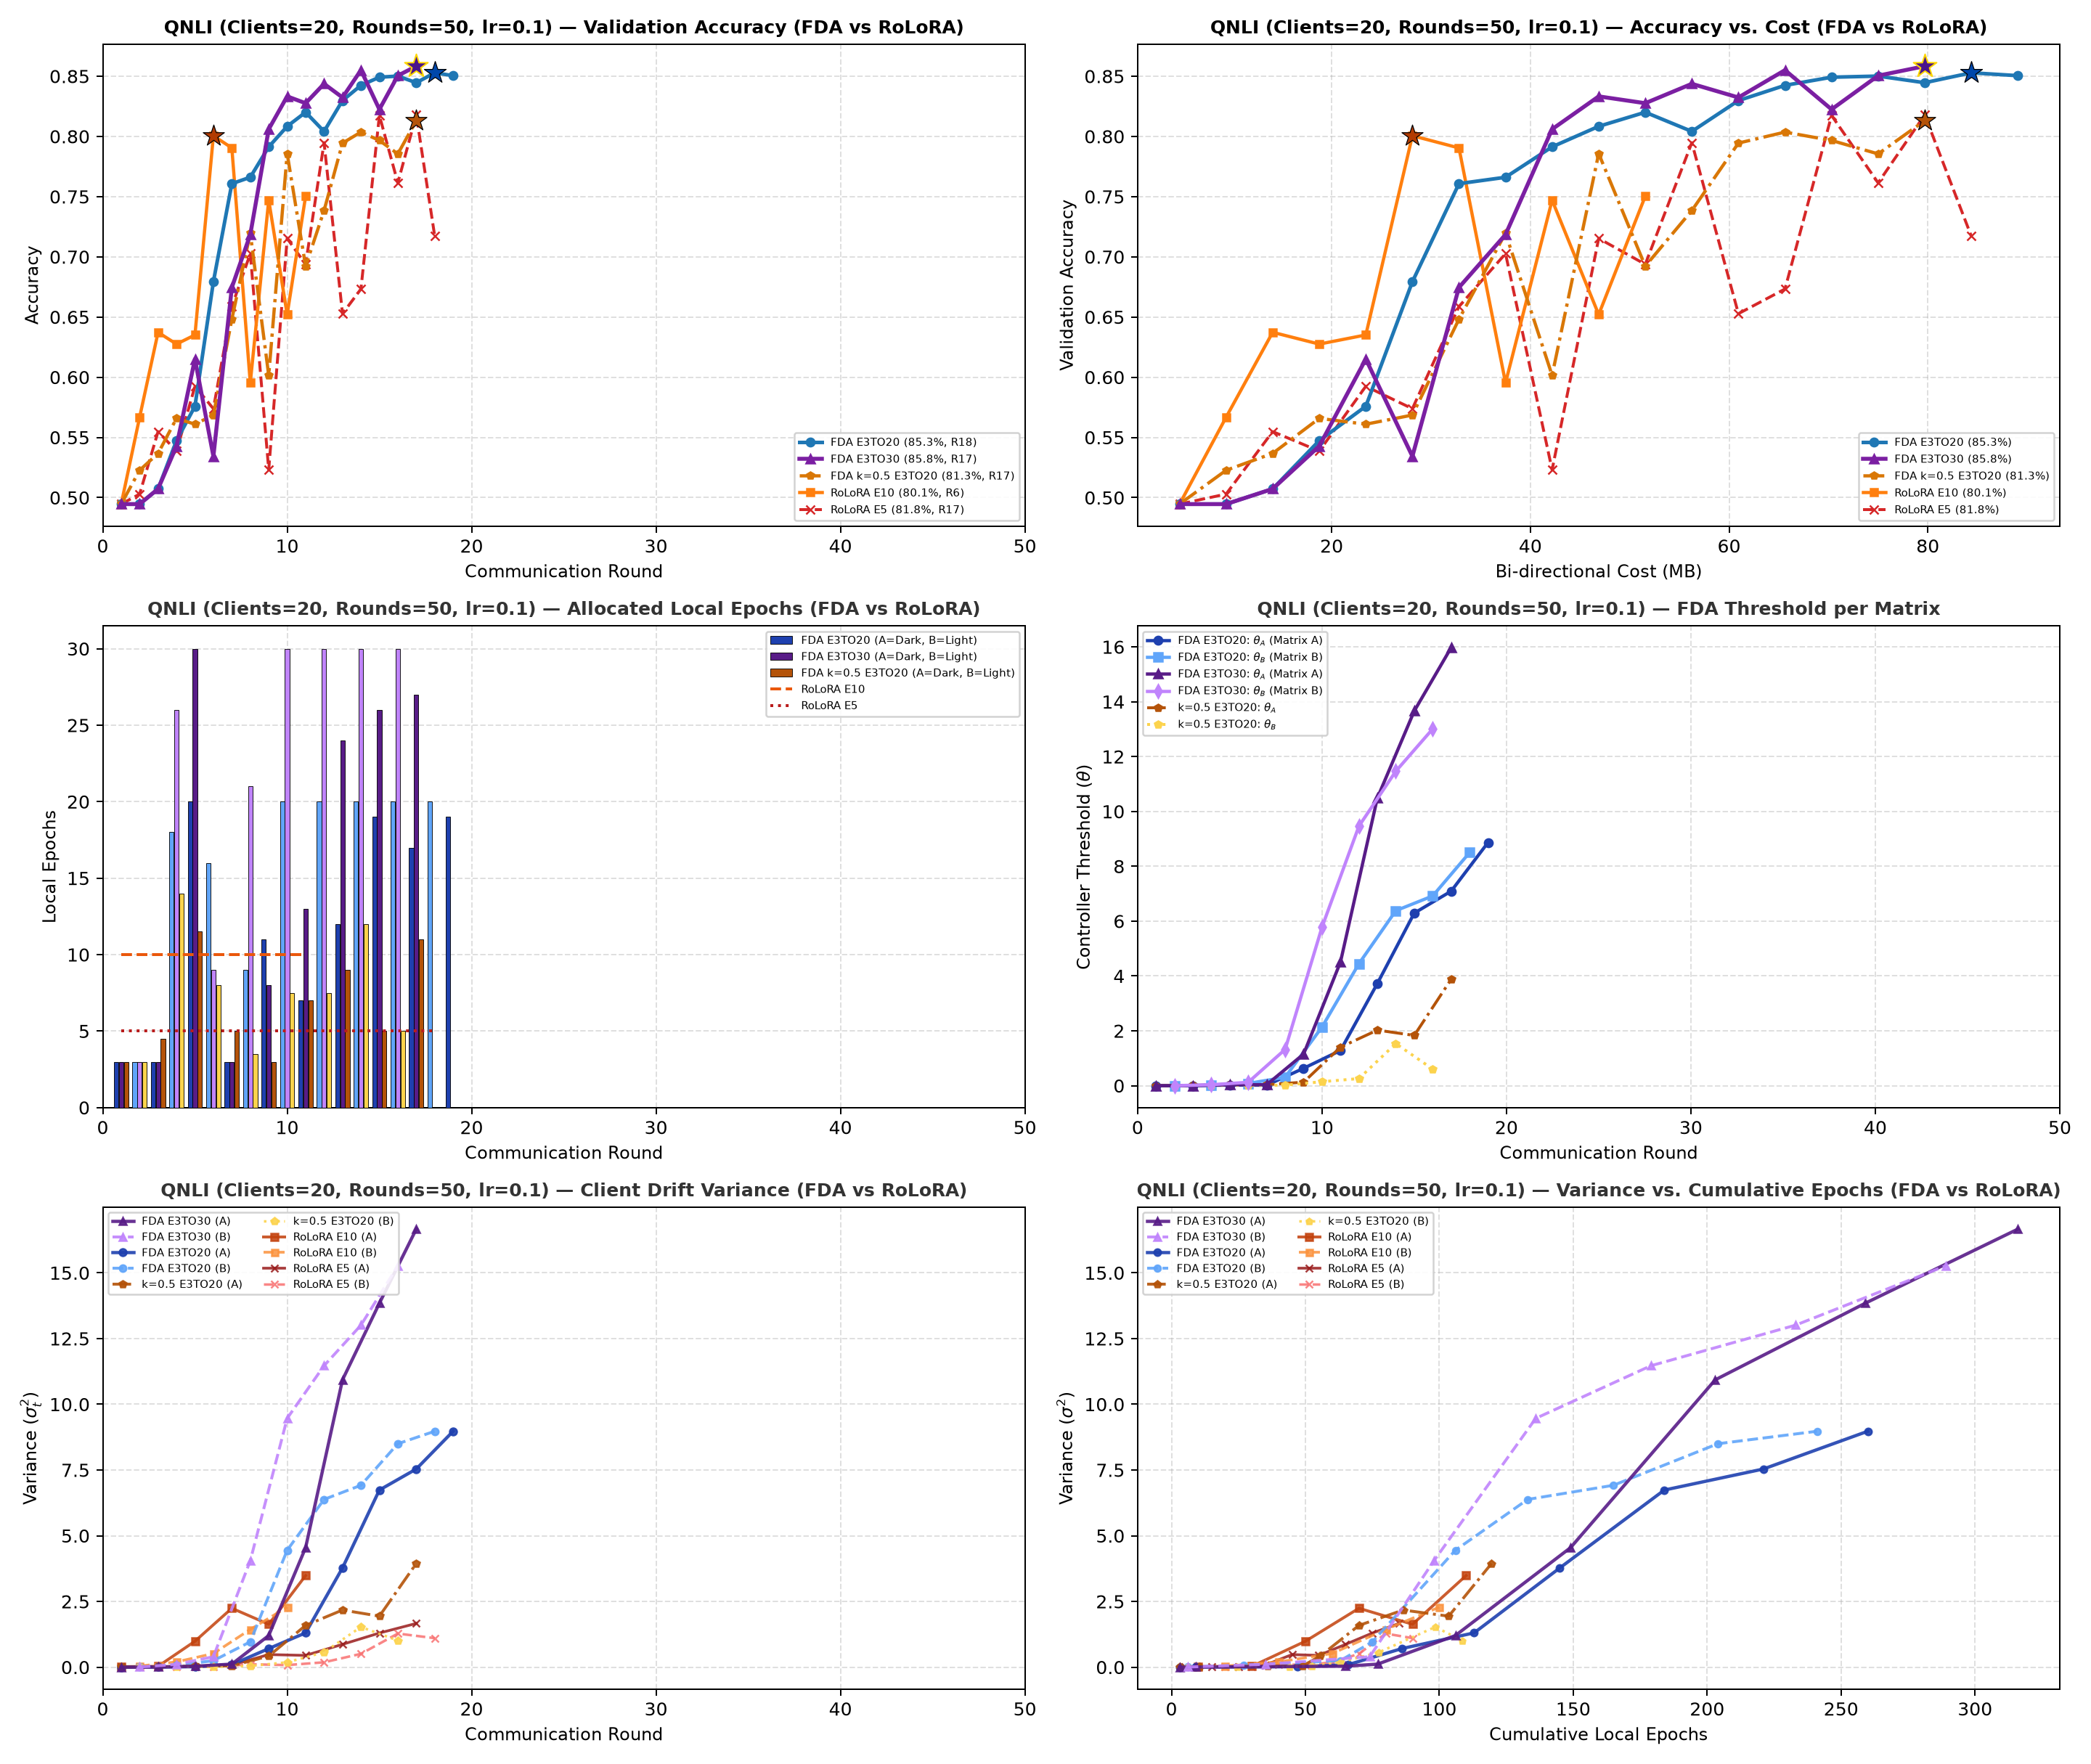
\includegraphics[width=\textwidth,height=0.62\textheight,keepaspectratio]{figures/05_QNLI_C20_R50_LR0.1_all6_telemetry_stacked.png}\\[-0.1em]
            {\tiny \textbf{QNLI ($C=20$, IID)}}
        \end{column}
        \begin{column}{0.24\textwidth}
            \centering
            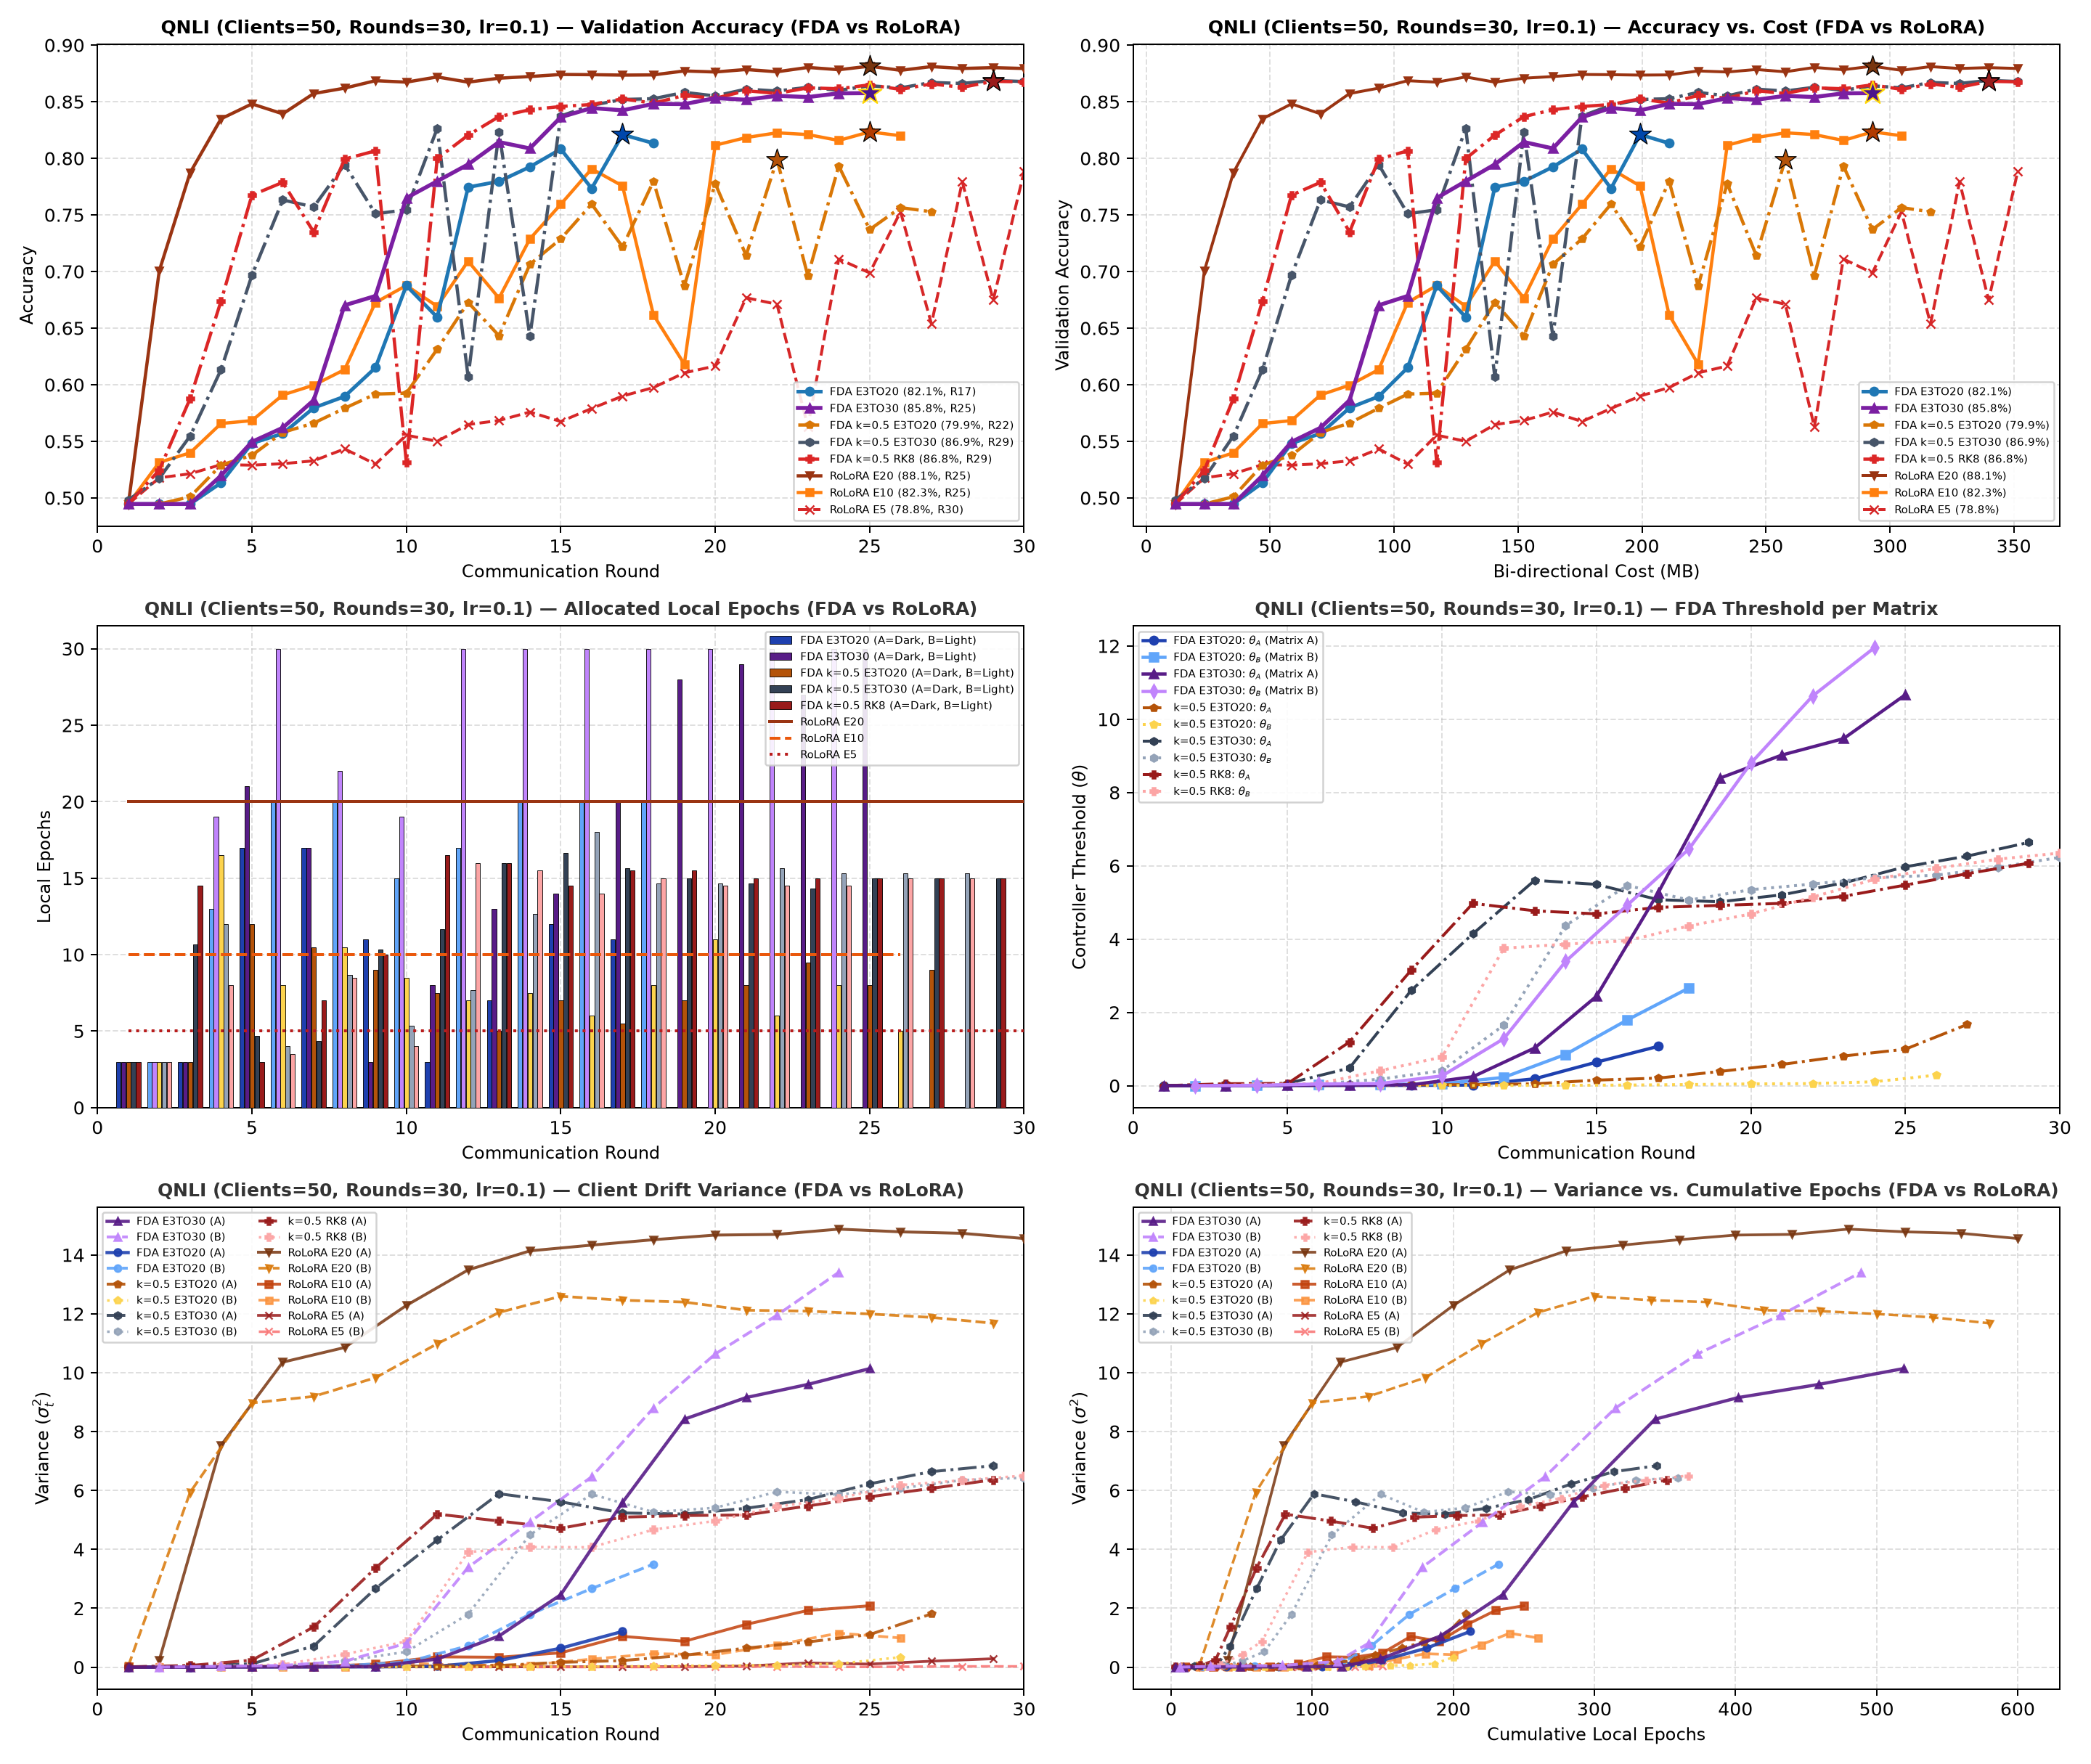
\includegraphics[width=\textwidth,height=0.62\textheight,keepaspectratio]{figures/07_QNLI_C50_R30_LR0.1_all6_telemetry_stacked.png}\\[-0.1em]
            {\tiny \textbf{QNLI ($C=50$, IID)}}
        \end{column}
    \end{columns}
\end{frame}

\begin{frame}[noframenumbering, label=backup_iid_qqp_sst2]{Backup : Additional IID Plots (QQP \& SST-2)}
    \framesubtitle{Multi-Panel Optimization Plots Under Homogeneous Consensus ($\alpha=1000.0$) \hfill \hyperlink{main_iid}{\beamerreturnbutton{Back to IID}} \; \hyperlink{thank_you}{\beamerreturnbutton{Q\&A}}}
    \vspace{-0.4em}
    \begin{columns}[c]
        \begin{column}{0.32\textwidth}
            \centering
            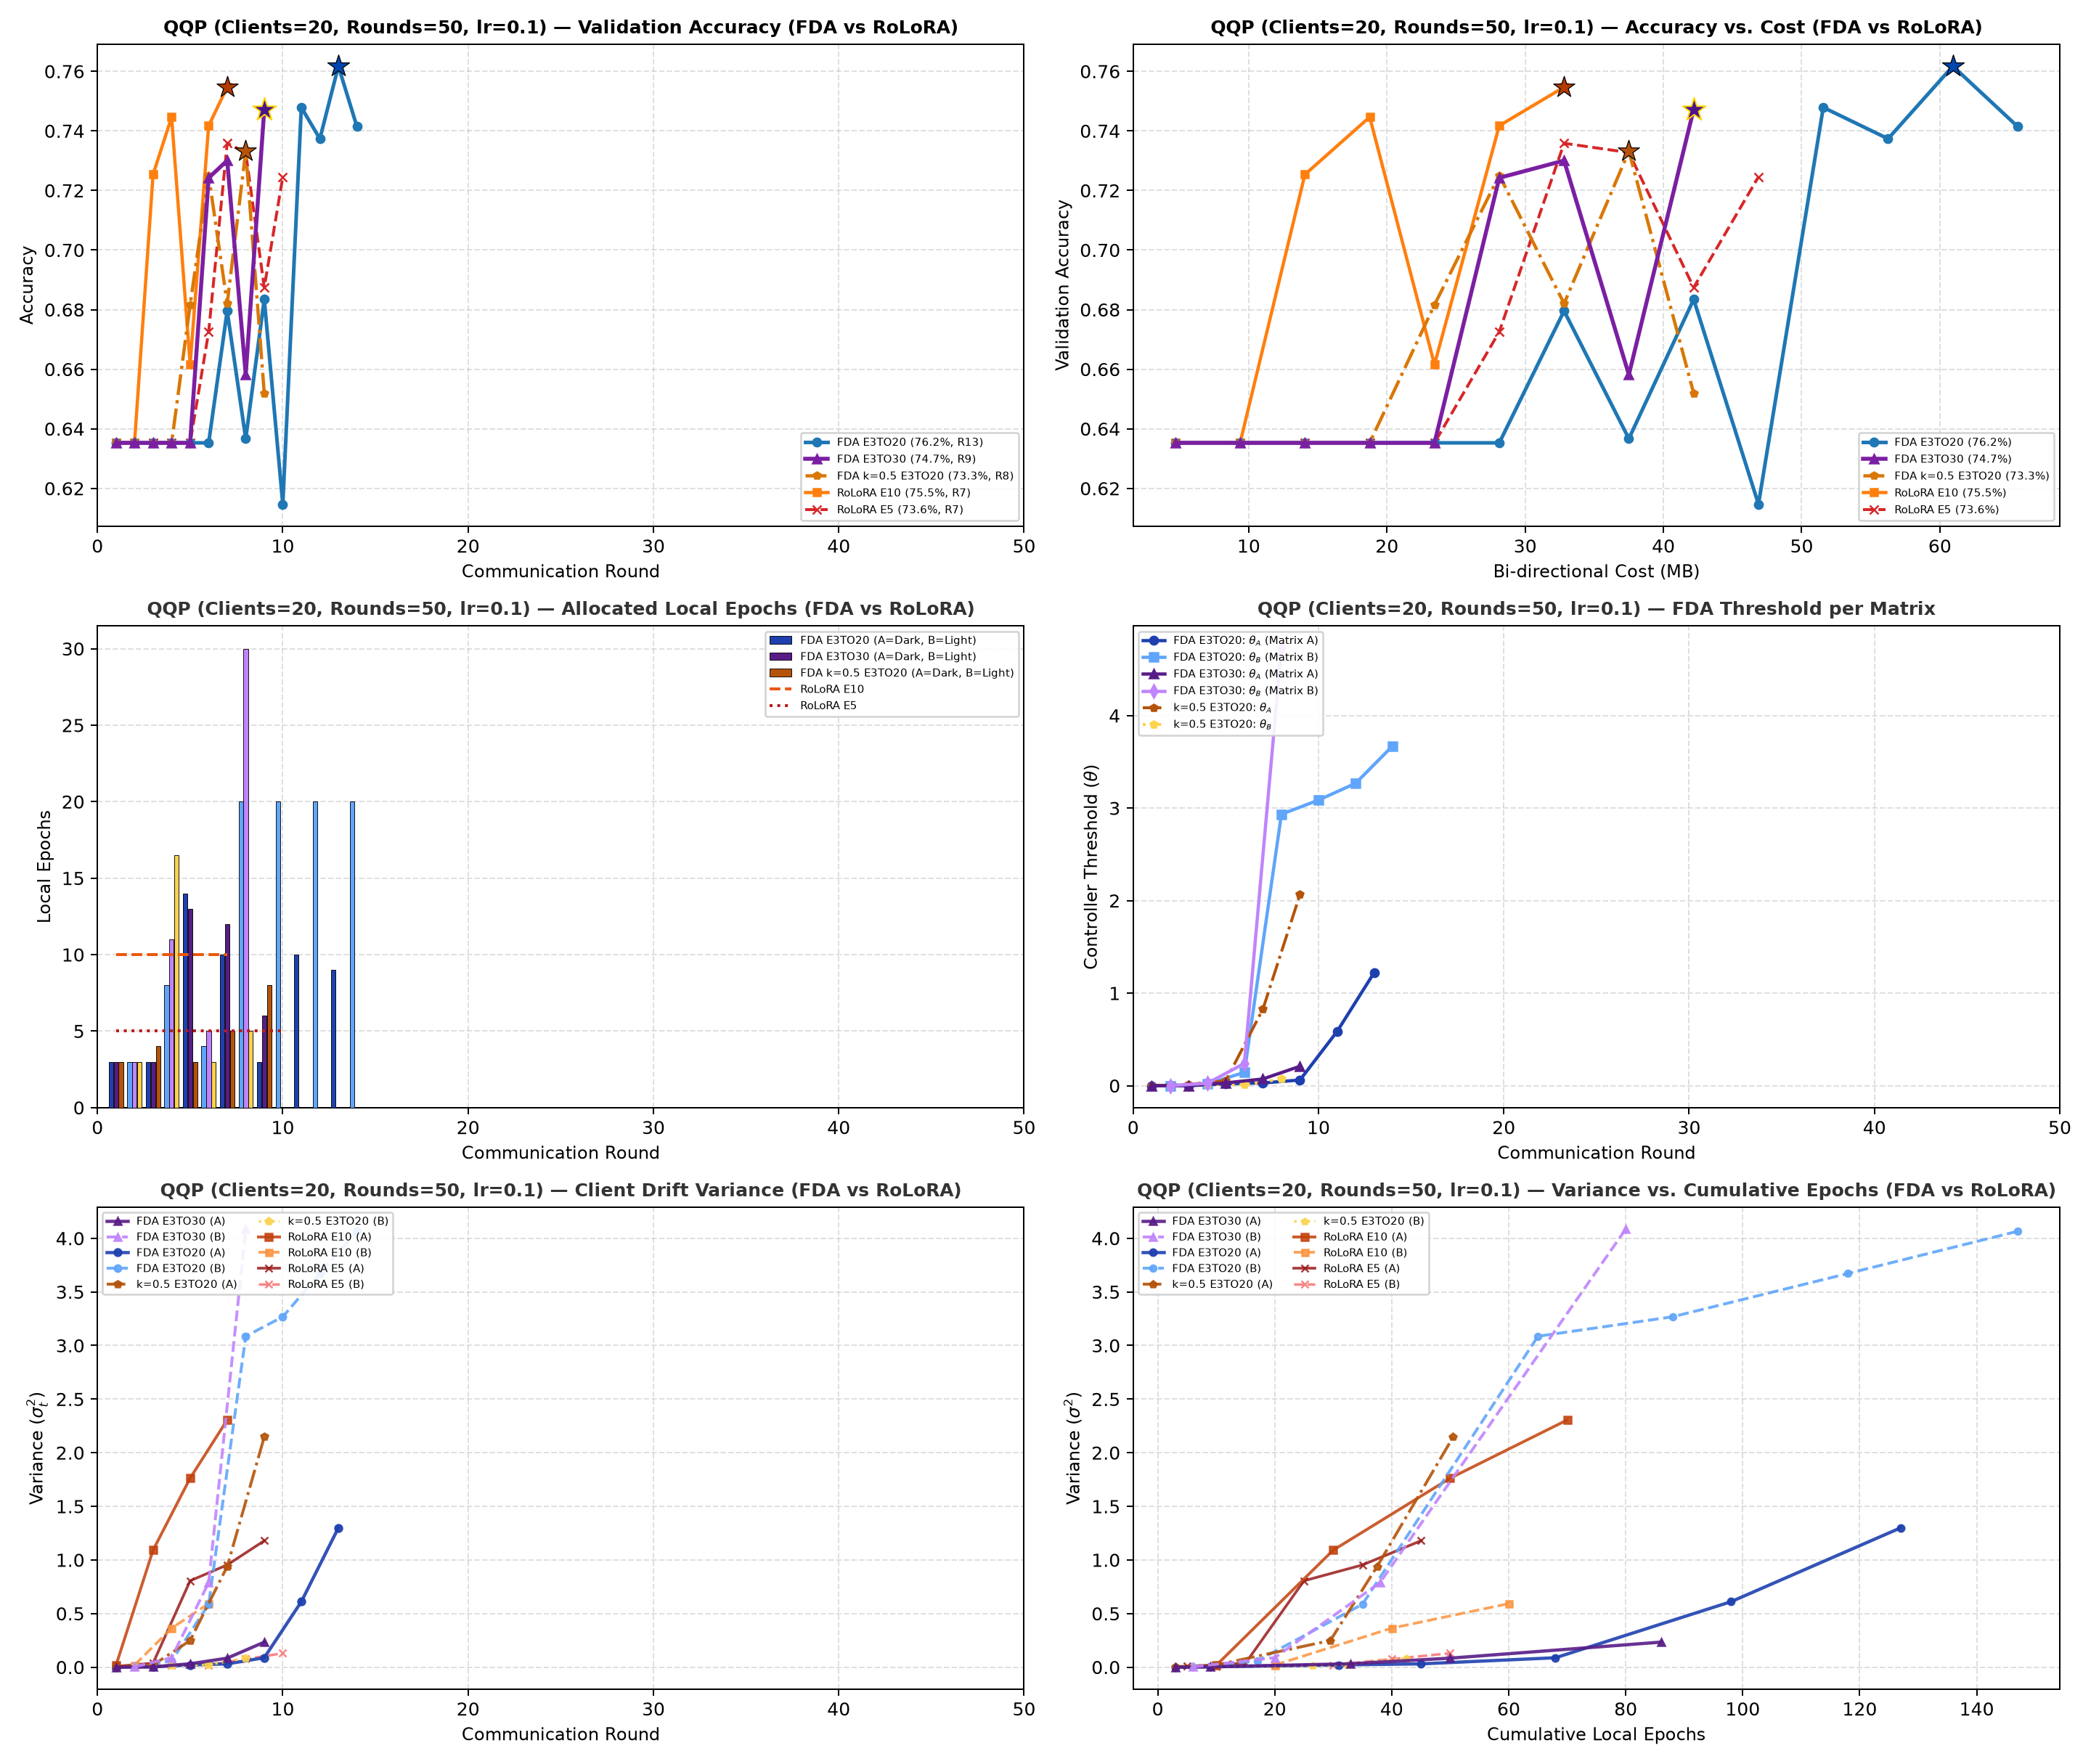
\includegraphics[width=\textwidth,height=0.62\textheight,keepaspectratio]{figures/09_QQP_C20_R50_LR0.1_all6_telemetry_stacked.png}\\[-0.1em]
            {\tiny \textbf{QQP ($C=20$, IID)}}
        \end{column}
        \begin{column}{0.32\textwidth}
            \centering
            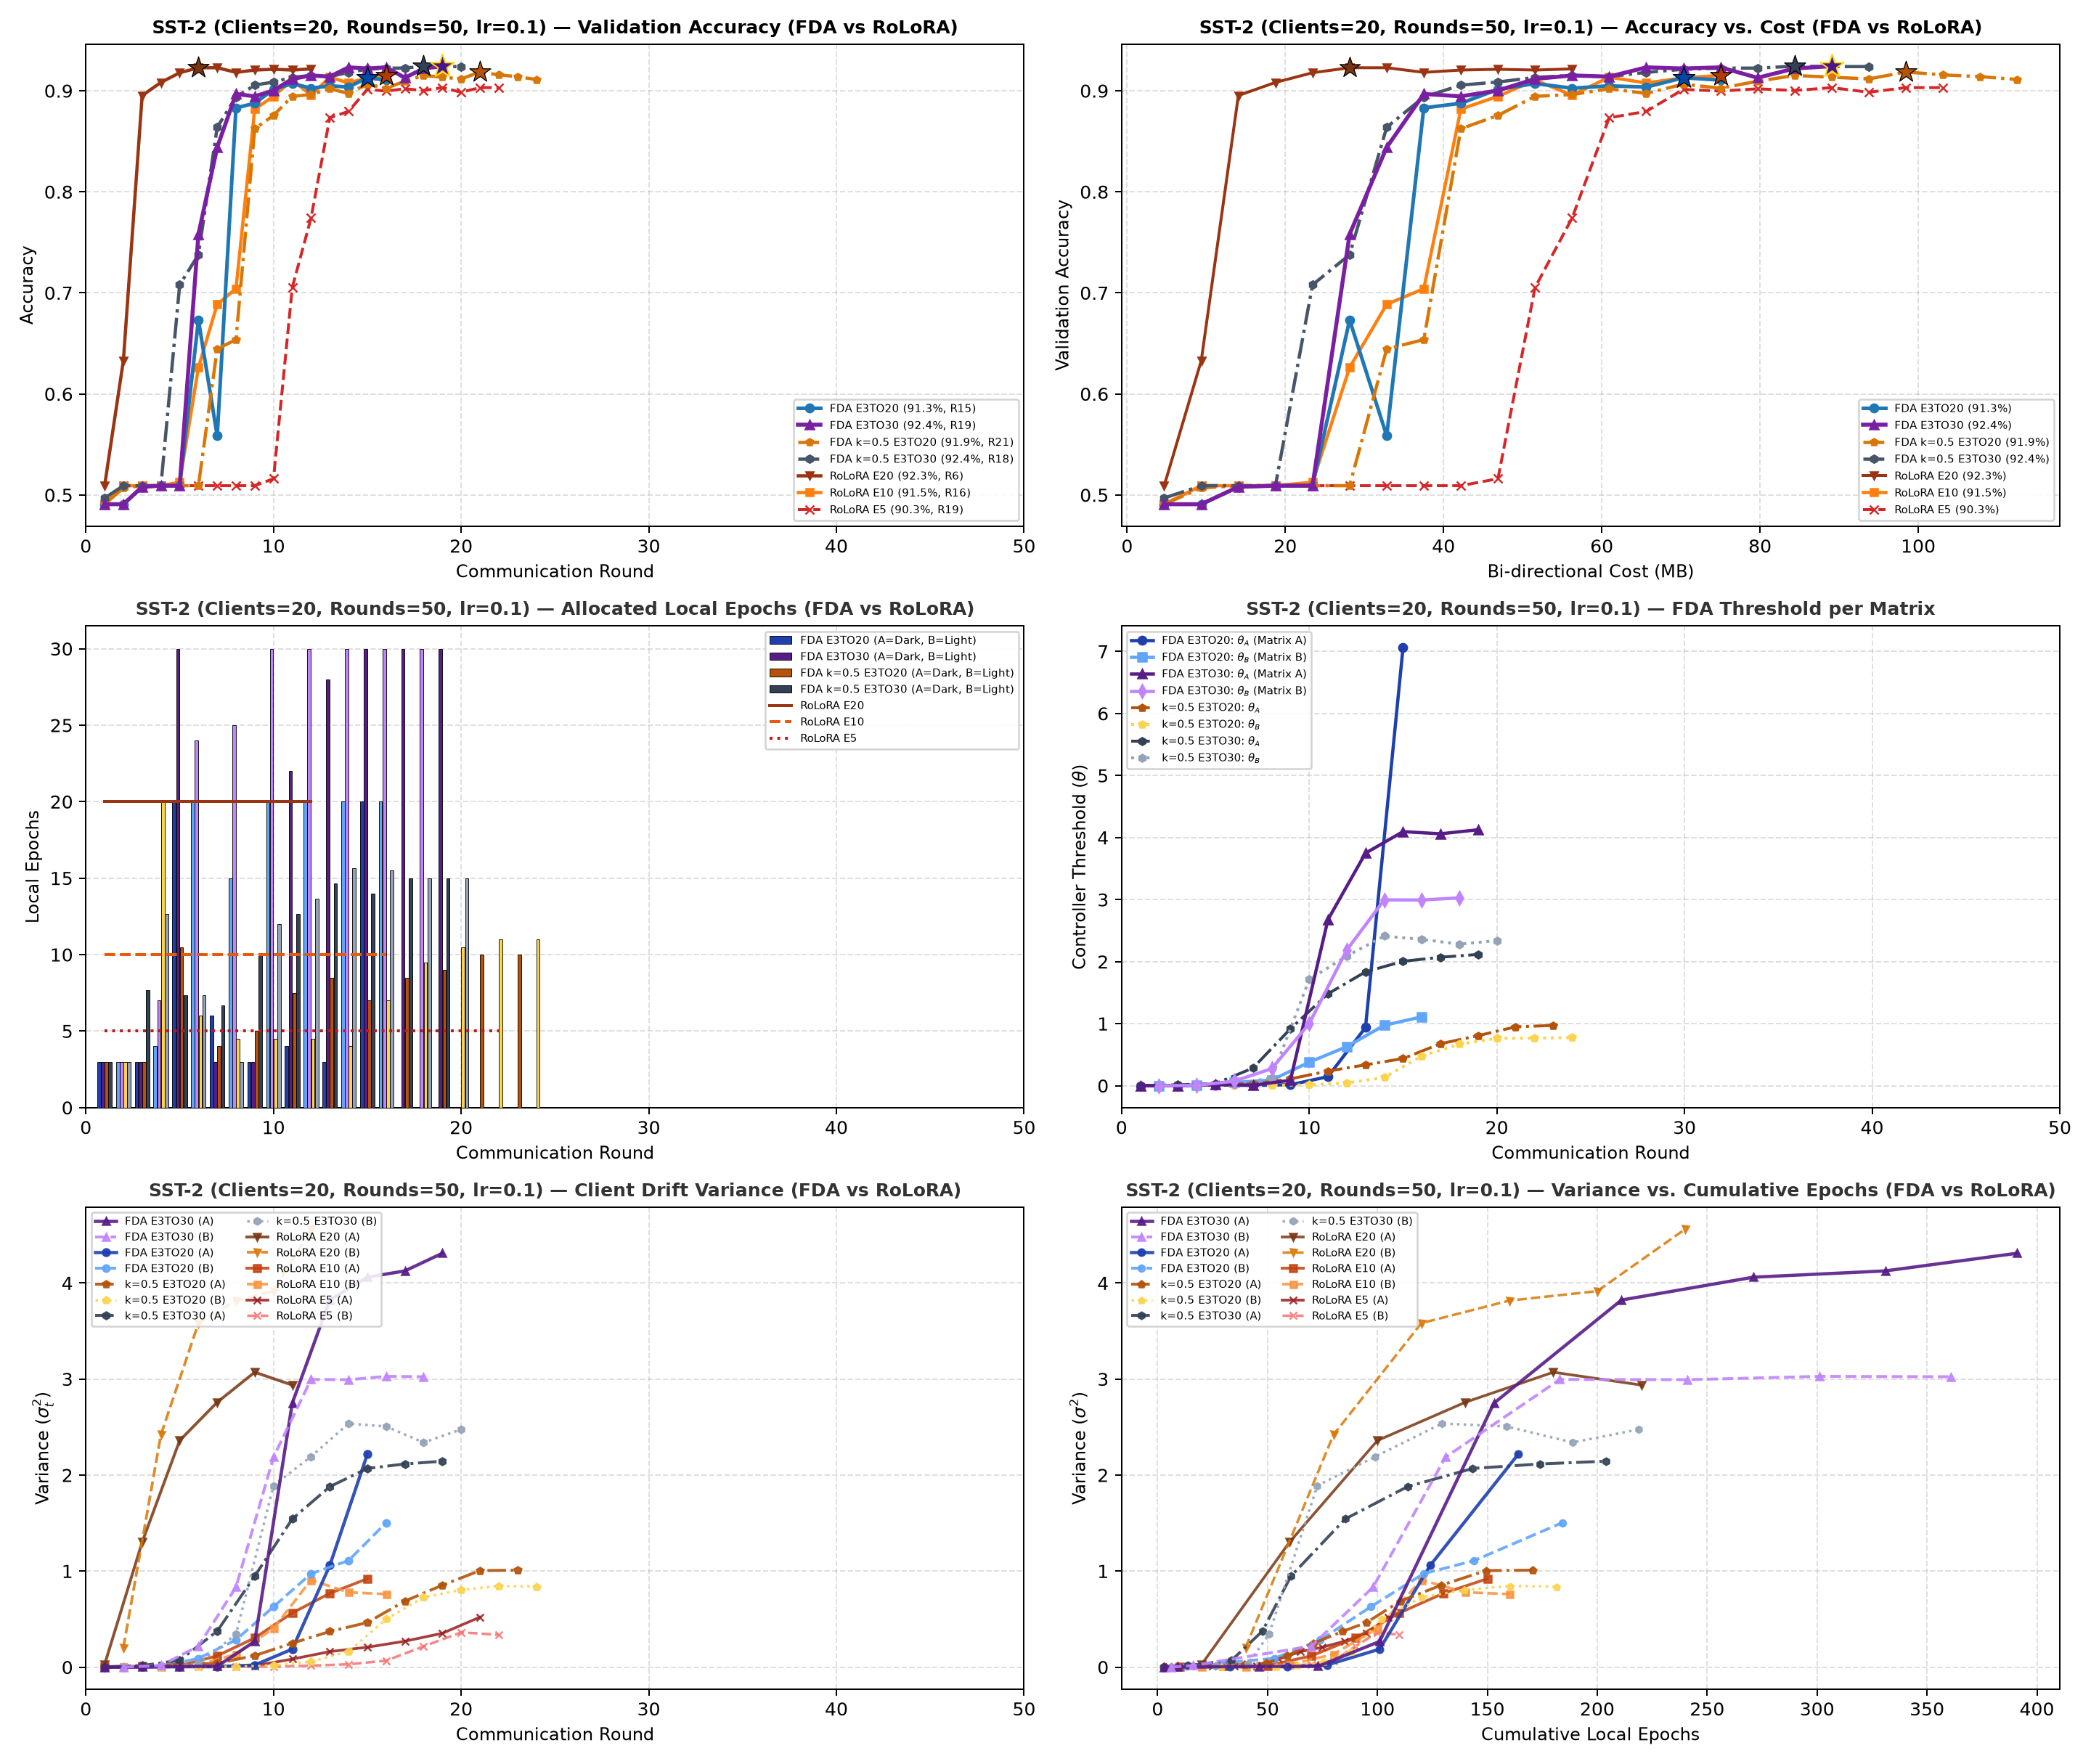
\includegraphics[width=\textwidth,height=0.62\textheight,keepaspectratio]{figures/11_SST2_C20_R50_LR0.1_all6_telemetry_stacked.png}\\[-0.1em]
            {\tiny \textbf{SST-2 ($C=20$, IID)}}
        \end{column}
        \begin{column}{0.32\textwidth}
            \centering
            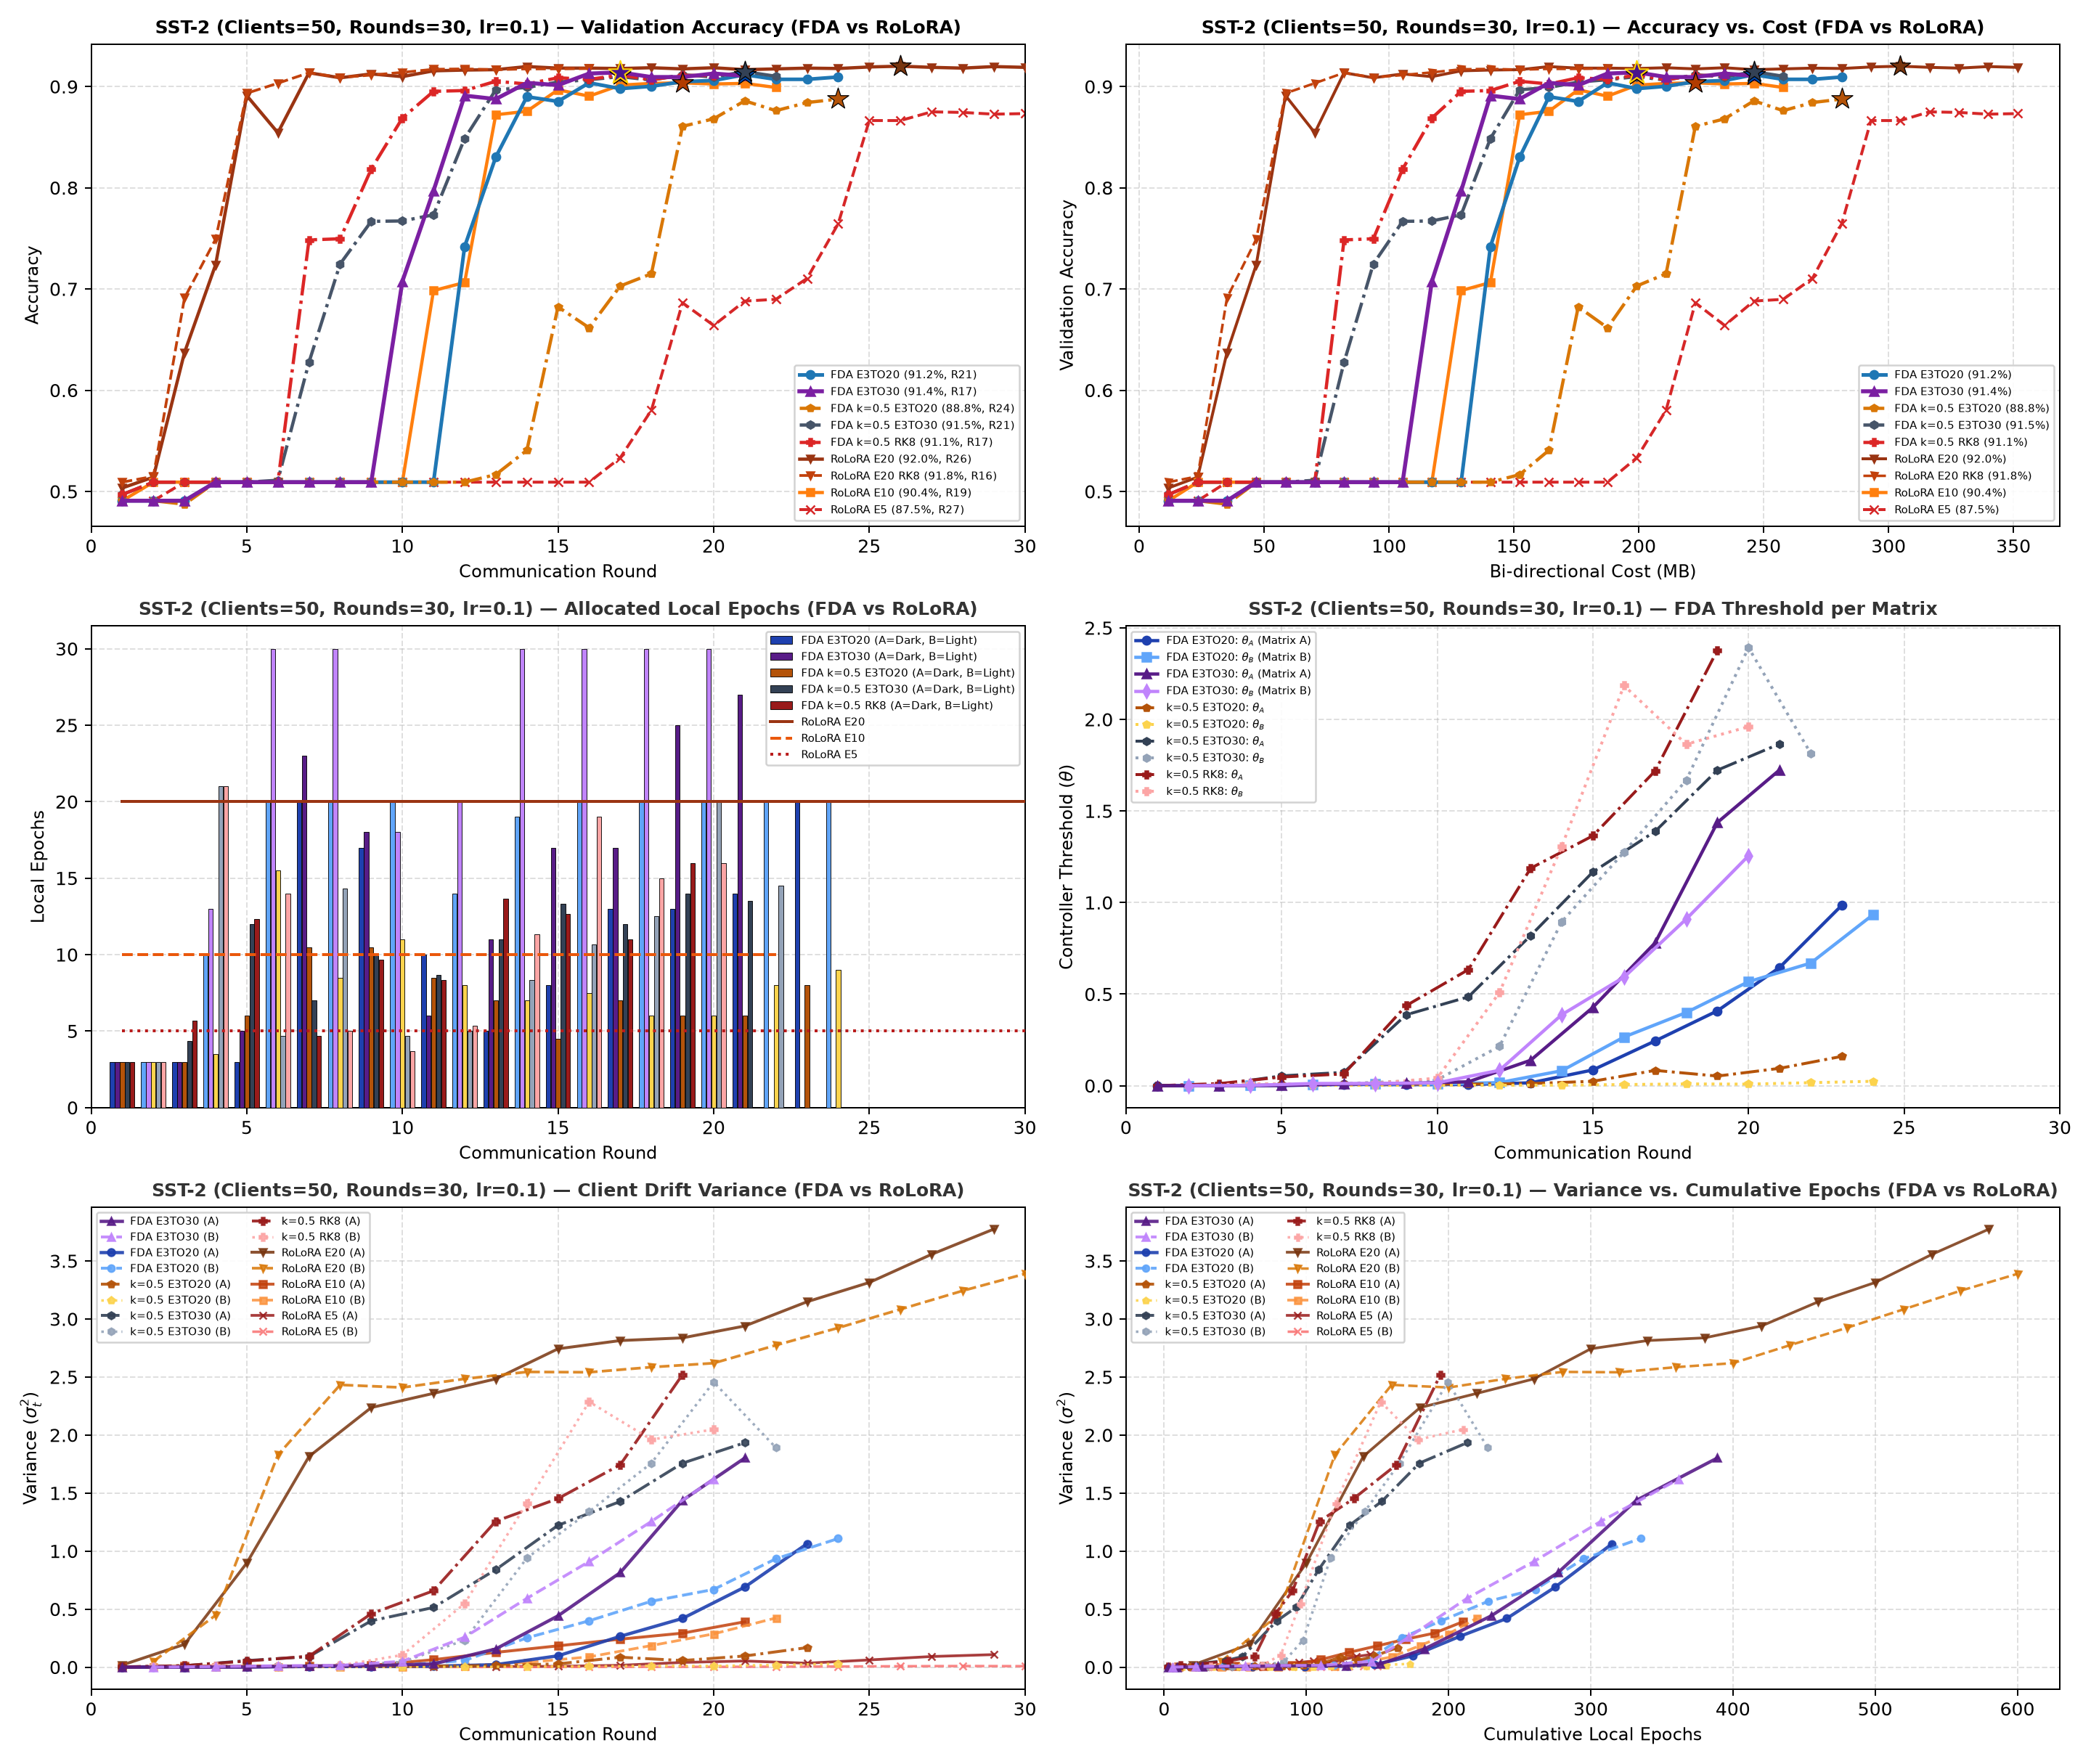
\includegraphics[width=\textwidth,height=0.62\textheight,keepaspectratio]{figures/12_SST2_C50_R30_LR0.1_all6_telemetry_stacked.png}\\[-0.1em]
            {\tiny \textbf{SST-2 ($C=50$, IID)}}
        \end{column}
    \end{columns}
\end{frame}

\end{document}
